\documentclass{article}


\usepackage{amsmath}
\usepackage{amsthm}
\usepackage{amssymb,latexsym,color}
\usepackage{mdwlist}
\usepackage{fullpage}
\usepackage{charter}
\usepackage{tikz}
\usepackage{url}



\usepackage{algorithm}
\usepackage[noend]{algpseudocode}

\usepackage{fullpage}
\usepackage{marvosym}
%\usepackage[techreport]{systems-cover}

\usepackage{graphicx}
\graphicspath{ {Figures/} }
\usepackage{subcaption}
%\captionsetup[subfigure]{justification=justified,singlelinecheck=false}


\usepackage{amsfonts}
\usepackage{comment}
\usepackage{listings}
\usepackage{balance}
\usepackage{cmtt}
\usepackage{subfig}
\usepackage{tabularx}
\usepackage{tikz}
\usepackage{pgfplots, pgfplotstable}
\usepackage{mathtools}

\newcommand{\R}{\mathsf{R}}
\newcommand{\sgn}[1]{\mbox{sgn}(#1)}
\renewcommand{\vec}[1]{\mathbf{#1}}
\newcommand{\poly}{\mathrm{poly}}

\newcommand*\circled[1]{\tikz[baseline=(char.base)]{
\node[shape=circle,draw,color=black,text=black,inner sep=0.05pt](char){#1};}}

\def\a{{\bf a}}
\def\g{{\bf g}}
\def\x{{\bf x}}
\def\y{{\bf y}}
\def\w{{\bf w}}
\def\E{\mathbb{E}}
\def\rrow{r_\mathrm{row}}

\newcommand{\err}{\ensuremath{\mathrm{err}}}
\newcommand{\setX}{\Omega}
\newcommand{\setI}{\mathcal{I}}
\newcommand{\OPT}{\ensuremath{\mathrm{OPT}}}
\newcommand{\setF}{\mathcal{F}}
\newcommand{\setJ}{\mathcal{J}}


\DeclareMathOperator*{\argmin}{argmin}

\newtheorem{lemma}{Lemma}
\newtheorem{theorem}{Theorem}
\newtheorem{claim}{Claim}
\newtheorem{corollary}{Corollary}
\newtheorem{prop}{Proposition}
\newtheorem{definition}{Definition}

\newcommand{\todo}[1]{\noindent \textbf{[TODO:] #1 } }
\usepackage{mathtools}
\DeclarePairedDelimiter\floor{\lfloor}{\rfloor}
\DeclarePairedDelimiter\ceil{\lceil}{\rceil}
%\newcommand{\E}{\mathbb{E}}

%\input{settings-custom.tex} 
%\linespread{0.95}
%\includepackage{algorithm}




\date{}


\title{\Large \bf
Supplementary Material
}

\begin{document}
\maketitle

\section{Preliminaries}

\subsection{Computational Model}

We consider a computational model illustrated in
Figure~\ref{fig:model}.  
In this context, SGD is often bounded by the bandwidth
of data movements cross these components. 
In particular, we consider the convergence properties of the algorithm when a lossy compression scheme is applied to the data (samples), 
gradient, and model, for the purpose of reducing the communication cost of the algorithm. 
It is interesting to consider how lossy compression impacts the update step in SGD. Let $Q( \vec{v} )$ denote the compression scheme applied to a vector $\vec{v}$. 

\begin{itemize}
    \item \textbf{Original iteration}: $$\x_{t + 1} \leftarrow \x_t - \gamma \g_k (\x_t, \vec{a}_t).$$
    \item \textbf{Compressed gradient}: $$\x_{t + 1} \leftarrow \x_t - \gamma Q( \g_k (\x_t, \vec{a}_t) ).$$
    \item \textbf{Compressed model}: $$\x_{t + 1} \leftarrow \x_t - \gamma \g_k (Q(\x_t), \vec{a}_t).$$
    \item \textbf{Compressed sample}: $$\x_{t + 1} \leftarrow \x_t - \gamma \g_k (\x_t, Q(\vec{a}_t)).$$
    \item \textbf{End-to-end compression}: $$\x_{t + 1} \leftarrow \x_t - \gamma Q(\g_k (Q(\x_t), Q(\vec{a}_t))).$$
\end{itemize}










\begin{figure*}[t]
\centering   
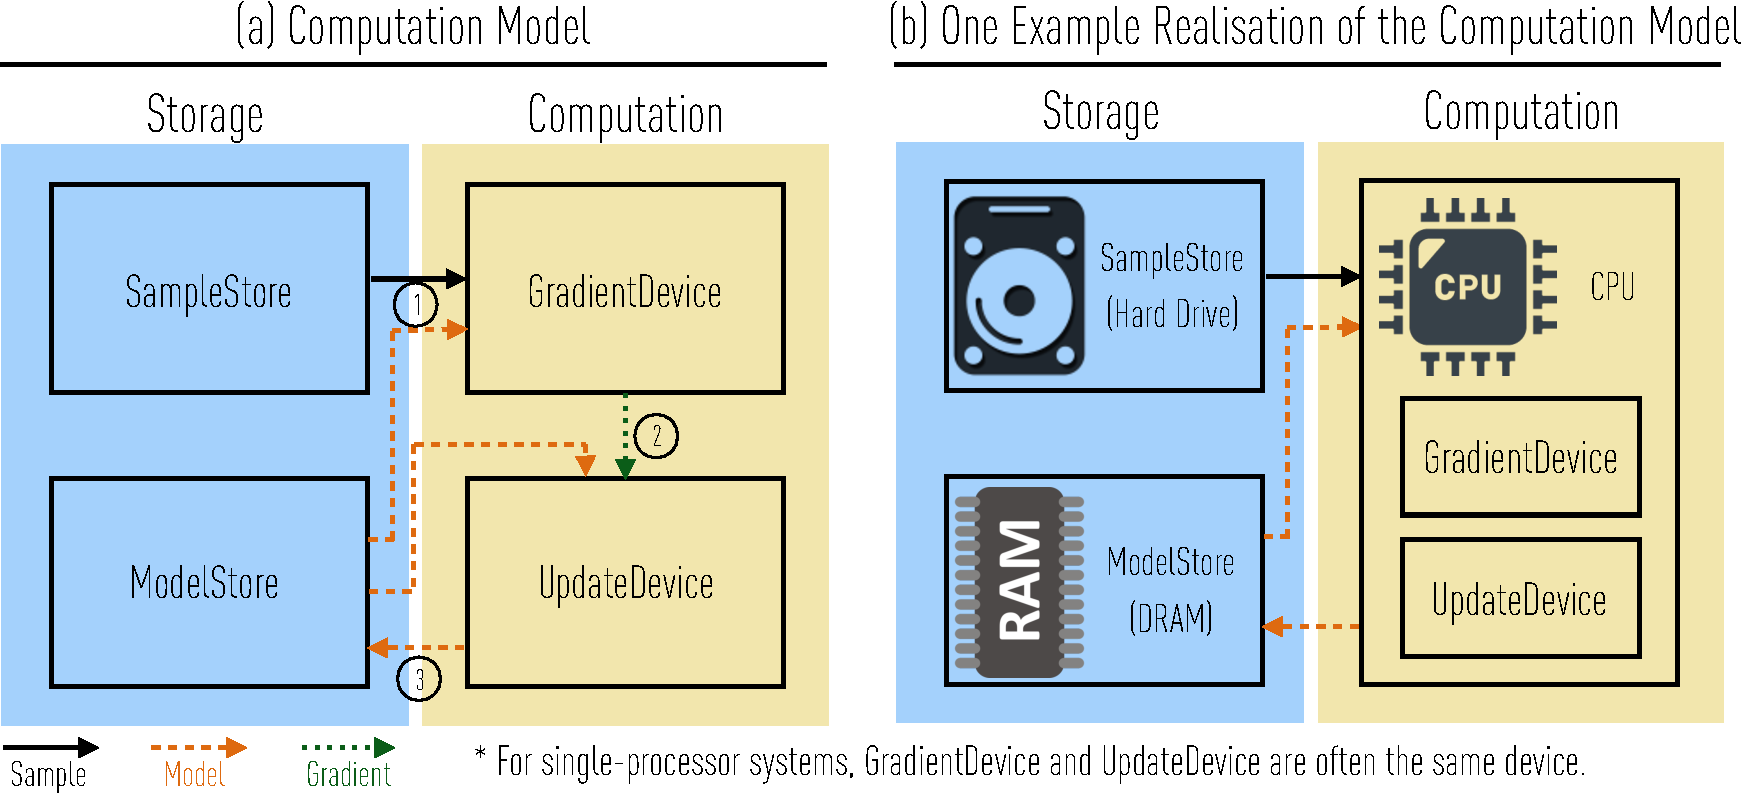
\includegraphics[scale=0.4]{compmodel-pdfcrop}
\caption{(a) A Schematic Representation of the Computation Model and (b) An Example Realisation
of the Computation Model. Three types of
data, namely (1) sample, (2) model, and (3)
gradient, moves in the system in three
steps as illustrated in (a). Given
different parameters of the computation model,
such as computational power and memory bandwidth, the system bottleneck may
vary. For example, in 
realisation (b) having a hard drive, DRAM, and a
modern CPU, it is likely that the  bottleneck when training 
a dense generalized linear model is the
memory bandwidth between SampleStore
and GradientDevice.}
\label{fig:model}
\end{figure*}






%\begin{figure}[h]
%\centering
%   
%    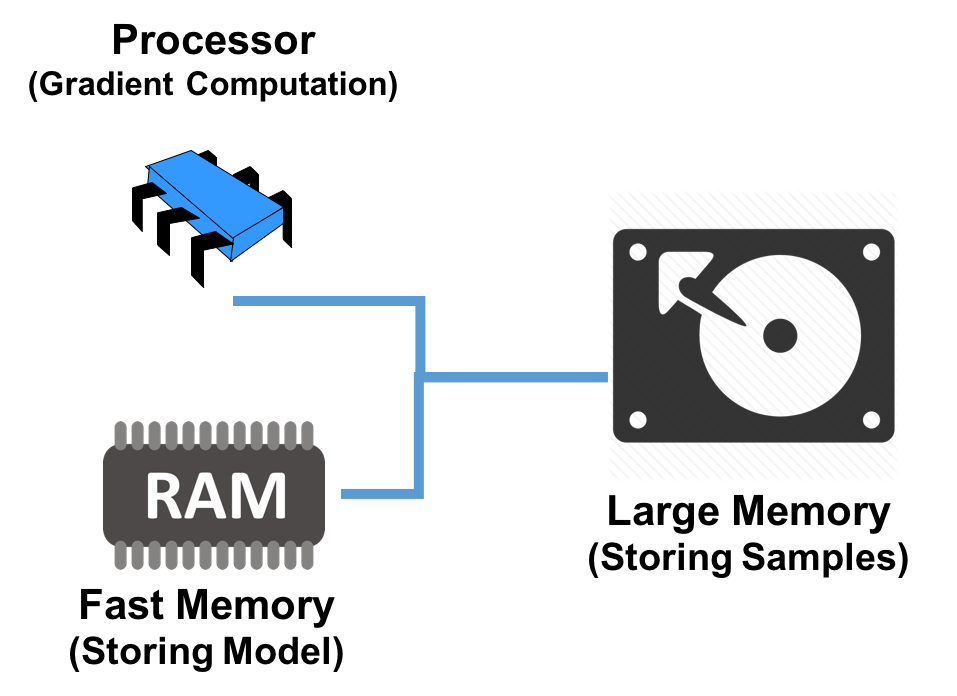
\includegraphics[scale=0.4]{schematic}
%    
%\caption{Simple Schematic of the %Computational Model}
%\label{fig:model}
%\end{figure}

\subsection{Guarantees for SGD}
In this paper we consider SGD, a general family of stochastic first order methods for finding the minima of convex (and non-convex) functions.
Due to its generality and usefulness, there is a vast literature on SGD in a variety of settings, with different guarantees in all of these settings.
Our techniques apply fairly generally in a black box fashion to many of these settings, and so for simplicity we will restrict our attention to a fairly basic setting.
For a more comprehensive treatment, see \cite{bubeck2015convex}.

Throughout the paper, we will assume the following setting in our theoretical analysis.
Let $\mathcal{X} \subseteq \R^n$ be a known convex set, and let $f: \mathcal{X} \to \R$ be differentiable, convex, and unknown.
We will assume the following, standard smoothness condition on $f$:
\begin{definition}[Smoothness]
Let $f: \R^n \to \R$ be differentiable and convex.
We say that it is $L$-smooth if for all $\x, \y \in \R^n$, we have
\[0 \leq f(\x) - f(\y) - \nabla f(\y)^T (\x - \y) \leq \frac{L}{2} \| \x - \y \|_2^2 \; .\]
\end{definition}

We assume repeated access to stochastic gradients, which on (possibly random) input $\vec{x}$, outputs a direction which is in expectation the correct direction to move in.
Formally:
\begin{definition}
Fix $f: \mathcal{X} \to \R$.
A \emph{stochastic gradient} for $f$ with bias bound $\beta$ is a random function $g (\x)$ so that $\E [g (\x) ] = G( \x)$, where $\| G(\x) - \nabla f(\x) \|_2 \leq \beta$ for all $x \in \mathcal{X}$.
%A \emph{stochastic oracle} for $f$ is an oracle which on (possibly random) input $\vec{x}$, outputs a stochastic gradient for $f$ at $\vec{x}$.
We say the stochastic gradient has second moment at most $B$ if $\E [\| g \|_2^2] \leq B$ for all $\x \in \mathcal{X}$.
We say it has variance at most $\sigma^2$ if $\E [\| g (\x) - \nabla f(\x) \|_2^2] \leq \sigma^2$ for all $\x \in \mathcal{X}$. 
\end{definition}

For simplicity, if $\beta = 0$ we will simply refer to such a random function as a stochastic gradient.
Under these conditions, the following convergence rate for SGD is well-known:

\begin{theorem}[e.g. \cite{2014arXiv1405.4980B}, Theorem 6.3]
\label{thm:sgd}
Let $\mathcal{X} \subseteq \R^n$ be convex, and let $f: \mathcal{X} \to \R$ be an unknown, convex, and $L$-smooth.
Let $\x_0 \in \mathcal{X}$ be given, and let $R^2 = \sup_{\x \in \mathcal{X}} \| \x - \x_0 \|_2^2$.
Suppose we run projected SGD on $f$ with access to independent stochastic gradients with bias bound $\beta$ and variance bound $\sigma^2$ for $T$ steps, with step size $\eta_t = 1 / ( L + \gamma^{-1})$, where $\gamma = \frac{R}{\sigma} \sqrt{\frac{2}{T}}$, and
\begin{equation}
\label{eq:sgd-conv}
T = O \left( R^2 \cdot \max \left( \frac{2 \sigma^2}{\epsilon^2} , \frac{L}{\epsilon} \right) \right) \; .
\end{equation}
Then $\E \left[ f \left( \frac{1}{T} \sum_{t = 0}^T \x_t \right) \right] - \min_{\x \in \mathcal{X}} f(\x) \leq \epsilon + R \beta + \frac{\eta}{2} \beta^2$.
\end{theorem} 

In particular, note that the complexity the SGD method is mainly controlled by the variance bound $\sigma^2$ we may obtain. If $\sigma = 0$, the complexity is consistent with the stochastic gradient.


\subsection{Randomized Quantization}

In this section, we give a procedure to quantize a vector or real values randomly, reducing its information content. We will denote this quantization function by $Q(\vec{v},s)$, where $s\geq 1$ is the tuning parameter. 
Let $M(\vec{v}): \R^n \rightarrow \R^n$ be a positive scaling function such that, for $\vec{v}\in \R^n$, $\frac{\vec{v}_i}{M_i(\vec{v})} \in [-1, 1]$, where $M_i(\vec{v})$ denotes the $i$th element of $M(\vec{v})$.
For $\vec{v} \neq \vec{0}$ we define

\begin{equation}
Q_i(\vec{v},s) = M_i(\vec{v}) \cdot \sgn{\vec{v}_i} \cdot \mu_i(\vec{v},s) \; , \label{equ:quant2}
\end{equation}
where $\mu_i(\vec{v},s)$'s are independent random variables defined as follows. 
Let $0 \leq \ell < s$ be an integer such that $|\vec{v}_i|/M_i(\vec{v}) \in [ \ell / s, (\ell + 1) / s ]$, that is, $\ell = \lfloor s |\vec{v}_i|/\| \vec{v} \| \rfloor$. 
Here, $p(x,s) = x s - \ell$ for any $x \in [0,1]$.
Then 
\[
\mu_i(\vec{v},s) = \left\{ \begin{array}{ll}
         \ell / s & \mbox{with probability $1 - p\left(\frac{|\vec{v}_i|}{M(\vec{v})},s\right)$};\\
         (\ell + 1) / s & \mbox{otherwise}. \end{array} \right.
\]
If $\vec{v} = \vec{0}$, then we define $Q(\vec{v},s) = \vec{0}$.
For any such choice of $M_i$, we have the following properties, which generalize Lemma 3.4 in~\cite{Alistarh:2016:ArXiv}.
The proofs follow immediately from those in \cite{Alistarh:2016:ArXiv}, and so we omit them for conciseness.
\begin{lemma}
\label{lem:quant-facts}
 For any $\vec{v} \in \R^n$, we have that 
 \begin{itemize} 
 \item (Sparsity) $\E[ \|Q(\vec{v}, s)\|_0]\leq
 s^2 +\sqrt{n}$ , 
 \item (Unbiasedness) $\E [Q (\vec{v},s)] = \vec{v}$ , and
 \item (Second Moment Bound) 
$\E [\| Q (\vec{v},s) \|_2^2] \leq r M^2$, where $M = \max_i M_i (\vec{v})$, and 
\[
r = r(s) = \left( 1 + \frac{1}{s^2} \sum_{i = 1}^n p\left( \frac{|\vec{v}_i|}{M_i },s \right) \right) \; .
\]
 \end{itemize}
\end{lemma}


We now discuss different choices of the scaling function $M_i(\vec{v})$.

\paragraph*{``Row Scaling''}

One obvious choice that was suggested in \cite{Alistarh:2016:ArXiv} is to have $M_i(\vec{v}) = \| \vec{v} \|_2$, in this way, we
always have $\frac{\vec{v}_i}{M_i(\vec{v})} \in [-1, 1]$ and all $M_i(\vec{v})$ are the same
such that we can store them only once.
When the 
In the following, we will often use the version with $s = 1$, which is as follows. 
\begin{equation}
\label{equ:quant1}
Q_i(\vec{v}) = \| \vec{v} \|_2 \cdot \sgn{\vec{v}_i} \cdot \mu_i (\vec{v}) \; ,
\end{equation}
where $\mu_i(\vec{v})$'s are independent random variables such that $\mu_i(\vec{v}) = 1$ with probability $|\vec{v}_i| / \| \vec{v} \|_2$, and $\mu_i(\vec{v}) = 0$, otherwise. If $\vec{v} = \vec{0}$, we define $Q(\vec{v}) = \vec{0}$. 
%
Obviously, if
all vectors $\vec{v}$ are scaled to have unit $\ell_2$ norms, $M(\vec{v}) \equiv 1$
and therefore, we can also omit this term.
Moreover, it was shown in \cite{Alistarh:2016:ArXiv} that for this choice of $M_i$, the function $r$ can be upper bounded by
\[
r(s) \leq \rrow (s) = 1 + \min\left( \frac{n}{s^2}, \frac{\sqrt{n}}{s} \right) \; .
\]

\paragraph*{``Column Scaling''}
Let $\vec{v} \in \R^n$ be a sample and $V \subset \R^n$ be the set of sample vectors. 
%Another choice, especially when $\vec{v} \in \R^n$ is an input sample and 
We can obtain the upper and lower bound for each feature, that is,
%$the {\em constant} for each $\vec{v}_i$ such that Another choice, especially when $\vec{v} \in \R^n$ is an input sample and we know the {\em constant} for each $\vec{v}_i$ such that 
\[
\text{min}_i \le \vec{v}_i \le  \text{max}_i\quad \vec{v} \in V
\]
is to have $M_i(\vec{v}) = \max(|\text{min}_i|, |\text{max}_i|)$.
When the input samples are stored as a matrix in which each row corresponds
two a vector $\vec{v}$, getting $\min_i$ and $\max_i$
is just to getting
the $\min$ and $\max$ for each column (feature).
Using this scheme, all input samples can share the same
$M_i(\vec{v})$ and thus can be easily stored in cache when all
input samples are accessed sequentially (like in SGD).


\paragraph*{Choice between Row Scaling and Column Scaling}

In this working paper, we make the following choices regarding row scaling
and column scaling and leave the more general treatment to future work.
For all input samples, we always use column scaling because it is easy
to calculate $M_i$ which does not change during training. For all gradients
and models, we use row scaling because the range of values is more dynamic.

\section{Compressing the Samples for Linear Regression}

In this section, we will describe lossy compression schemes for data samples, so that when we apply SGD to solve linear regression on these compressed data points, it still provably converges.
Throughout this section, the setting will be as follows.
We have labeled data points $(\a_1, b_1), (\a_2, b_2), \ldots, (\a_K, b_K) \in \R^n \times \R$, and our goal is to minimize the function
\[
f(\x) = \frac{1}{K} \sum_{k = 1}^K \| \a_k^\top \x + b_k \|_2^2 \; ,
\]
i.e., minimize the empirical least squares loss.
The basic (unquantized) SGD scheme which solves this problem is the following: at step $\x_k$, our gradient estimator is $\g'_k = \a_{\pi(k)} (\a_{\pi(k)}^\top \x + b_{\pi(k)})$, where $\pi(k)$ is a uniformly random integer from $1$ to $m$.
In a slight abuse of notation we let $\a_k = \a_{\pi(k)}$ for the rest of the section.
Then it is not hard to see that $\E [\g'_k] = \nabla f(\x_k)$, and so this is indeed a stochastic gradient.

The rest of the section is now devoted to devising quantization schemes for $\g'_k$ when given access only to $\a_k$ and $b_k$, namely, given access only to the data points.

\subsection{Naive Random Quantization is Biased}

As a first exercise, we look at what happens when we work with the data directly in quantized form in the context of linear regression. 
The gradient becomes
\[
\g_k := Q(\a_k, s ) Q(\a_k, s)^\top \x + Q(\a_k, s) b_k.
\]
It is not hard to see that the expected value of this is in fact: 
\[
\E[\g_k] := \a_k \a_k^\top \x + \a_k b_k + D_{s, \a} \x, 
\]
where $D_{s, \a}$ is a diagonal matrix and its $i$th diagonal element is 
\[
%D_{s, \a} = 
\E[ Q(\a_i, s)^2 ] - \a_i^2.
\]

Since $D_{s, \a}$ is non-zero, we obtain a \emph{biased} estimator of the gradient, so the iteration is unlikely to converge. 
In fact, it is easy to see that in instances where the minimizer $\x$ is large and gradients become small, we will simply diverge. 
Fortunately, however, this issue can be easily fixed. 

\subsection{Double Sampling}

\paragraph{Algorithm}
Instead of the naive estimate, our algorithm is as follows.
We generate two independent
random quantizations $Q_1$
and $Q_2$ and revise the gradient as follows:

%\[
%\g_k := \frac{1}{2}\left(Q_1(\a_k ) Q_2(\a_k)^\top \x + Q_2(\a_k) b_k + Q_2(\a_k ) %Q_1(\a_k)^\top \x + Q_1(\a_k) b_k\right).
%\]

%\[
%\g_k := Q_1 (\a_k, s) (Q_2 (\a_k, s)^\top \x + b_k) \; .
%\]
\[
\g_k := Q_1 (\a_k, s) (Q_2 (\a_k, s)^\top \x + b_k) \; .
\]
It is not hard to see that the above is an unbiased estimator of the true gradient.\footnote{In our implementation,
we used the average gradient $\g_k := \frac{1}{2}\left(Q_1 (\a_k, s) (Q_2 (\a_k, s)^\top \x + b_k) + 
Q_2 (\a_k, s) (Q_1 (\a_k, s)^\top \x + b_k)\right)$. This version does not impact  the upper bound in our variance analysis,
but enjoys lower variance (by a constant) both theoretically and empirically.}



\paragraph{Variance Analysis}

\begin{lemma} 
The stochastic gradient variance using double sampling above $\E\|\g_t - \g_t^{(full)}\|^2$ can be bounded by
\begin{align*}
%&\E\|\g_t - \g_t^{(full)}\|^2 \leq \\
&\Theta\left(\mathcal{TV}(\a_t) (\mathcal{TV}(\a_t)\|\x\odot \x\| + \|\a_t^\top \x\|^2 + \|\x\odot \x\|\|\a_t\|^2)\right),
\end{align*}
where $\mathcal{TV}(\a_t) := \E\|Q(\a_t) - \a_t\|^2$ and $\odot$ denotes the element product.
\end{lemma}
\begin{proof}
Let $\a$ denote $\a_t$ for short in the followed proof.
\begin{eqnarray*}
& & \E\left\|Q_1(\a)(Q_2(\a)^\top \x + b_t)\right\|^2
\\
& \leq & 
2\E\left\| (Q_1(\a)- \a) Q_2(\a)^\top \x \right\|^2 + 2\E\left\| \a(Q_2(\a) - \a)^\top \x) \right\|^2
\\
& \leq &
2 \E_1 \|Q_1(\a)-\a\|^2\E_2(Q_2(\a)^\top \x)^2 + 2 \|\a\|^2 \E((Q_2(\a)-\a)^\top\x)^2
\\
& \leq &
2 \E_1 \|Q_1(\a)-\a\|^2\E_2(Q_2(\a)^\top \x)^2 + 2 \|\a\|^2 \E((Q_2(\a)-\a)^\top\x)^2
\\
& \leq &
2 \mathcal{TV}(\a)(2 \|\a\|^2 \E((Q_2(\a)-\a)^\top\x)^2 + 2(\a^\top \x)^2)+ 2 \|\a\|^2 \E((Q_2(\a)-\a)^\top\x)^2
\\
& \leq &
\Theta\left(\mathcal{TV}(\a) (\mathcal{TV}(\a)\|\x\odot \x\| + \|\a^\top \x\|^2 + \|\x\odot \x\|\|\a\|^2)\right),
\end{eqnarray*}
which completing the proof.
\end{proof}

Let $r = r(s) = 1 + \min (n / s^2, \sqrt{n}/ s)$ be the blow-up in the second moment promised in Lemma \ref{lem:quant-facts}.
Then, we have the following lemma.
\begin{lemma}
    Let $\a_k, \x, b_k$ be fixed, and suppose that $\| \a_k \|_2^2 \leq A^2, \| \x \|_2^2 \leq R^2$, and $\max_i M_i (\a_k) \leq M_a$.
    Let $\g'_k = \a_k (\a_k^\top \x + b)$ be the (unquantized) stochastic gradient update.
    Then, we have 
    \[
    E_{Q_1, Q_2} [\| \g_k \|_2^2] \leq r \cdot \left( \| \g'_k \|_2^2 \cdot \frac{M_a^2}{\| \a_k \|_2^2} + \| \a_k \|_2^2 \frac{M_a^2}{s^2} R^2 \right)\; .
    \]
\end{lemma}
\begin{proof}
We have that 
\[
\E_{Q_1, Q_2}(\|\g_k\|^2) = \E_{Q_1, Q_2} [\| Q_1 (\a_k, s) (Q_2 (\a_k, s)^\top \x + b_k) \|_2^2].
\]
Next we have
\begin{align*}
    \E_{Q_1, Q_2} [\| Q_1 (\a_k, s) (Q_2 (\a_k, s)^\top \x + b_k) \|_2^2] &= \E_{Q_2} \left[ \E_{Q_1} [ (Q_2 (\a_k, s)^\top \x + b_k)^2 Q_1 (\a_k, s)^\top Q_1 (\a_k, s)] \right] \\
    &= \E_{Q_1}[ \| Q_1( \vec{a}_k, s) \|_2^2 ] \cdot \E_{Q_2} [\| \a_k (Q_2 (\a_k, s)^\top \x + b_k)\|_2^2 ] \\
    &\leq^{\mathrm{Lemma}~\ref{lem:quant-facts}} r M_a^2 \cdot \E [(Q_2 (\a_k, s)^\top \x + b_k)^2 ] \\
    &= r M_a^2 \left( \E [(Q_2 (\a_k, s)^\top \x)^2] + 2 b_k \E [Q_2 (\a_k, s)^\top \x] + b_k^2 \right) \\
    &= r M_a^2 \left( \E [(Q_2 (\a_k, s)^\top \x)^2] + 2 b_k \a_k^\top \x + b_k^2 \right)
\end{align*}
Moreover, we have
\begin{align*}
    E [(Q_2 (\a_k, s)^\top \x)^2] &= \x^\top \left( \E \left[ Q_2 (\a_k, s) Q_2 (\a_k, s)^\top \right] \right) \x \\
    &= \x^\top (\a_k \a_k^\top + D) \x^\top \\
    &\leq (\a_k^\top \x)^2 + \| D \|_{\mathrm{op}} \| \x \|_2^2 \; ,
\end{align*}
where $D = \mathrm{diag}_i [ (\E[Q_2 (\a_k, s)_i^2]) - (\a_k)_i^2 ] =\mathrm{diag}_i [ \mathrm{Var} [Q_2 (\a_k, s)_i] ].$ Further, we have that $\| D \|_{\mathrm{op}}  \leq M_a^2 / s^2$.
Therefore we have that:

\begin{align*}
     \E_{Q_1, Q_2} [\| Q_1 (\a_k, s) (Q_2 (\a_k, s)^\top \x + b_k) \|_2^2]  &\leq r M_a^2 \left( (\a_k^\top \x)^2 + \frac{M_a^2}{s^2} R^2 + 2 b_k \a_k^\top \x + b_k^2  \right) \\
    &= r \left( \| \g'_k \|_2^2 \cdot \frac{M_a^2}{\| \a_k \|_2^2} + \frac{A^2 M_a^2 R^2}{s^2} \right) \,
\end{align*}
as claimed, since $\| \g'_k \|_2^2 = \| \a_k \|_2^2 (\a_k^T \x + b_k)^2$.
\end{proof}
In particular, this implies the following variance bound on our quantized updates:
\begin{corollary}
\label{cor:var-bound}
    Let $\a_k, \x, b_k, \g'_k$ be as above.
    Suppose moreover $\E [\| \g'_k - \nabla f(\x_k) \|_2^2 ] \leq \sigma^2$ and $\E [\| \g'_k \|_2^2] \leq B$.
    Then, we have
    \[
    \E \left[ \| \g_k - \nabla f(\x_k) \|_2^2 \right] \leq  \sigma^2 + \left(r \frac{M_a^2}{\| \a_k \|_2^2} - 1\right) B + \frac{r A^2 M_a^2 R^2}{s^2} \; ,
    \]
    where the expectation is taken over $\g'_k$ and the randomness of the quantization.
\end{corollary}
\begin{proof}
    Observe that $\| \g_k - \nabla f(\x_k) \|_2^2 = \| \g_k - \g'_k \|_2^2 + 2 (\g_k - \g'_k)^\top (\g'_k - \nabla f(\x_k)) + \| g'_k + \nabla f(\x_k) \|_2^2$.
    Since $\E [(\g_k - \g'_k)^\top (\g'_k - \nabla f(\x_k))] = 0$, and by assumption $\E [ \| g'_k + \nabla f(\x_k) \|_2^2] \leq \sigma^2$, it suffices to bound the expectation of the first term.
    We have
    \[
     \E \left[ \| \g_k - \nabla f(\x_k) \|_2^2 \right] \leq 2 \sigma^2 + 2\E_{\g'_k} \left[ \E_{Q_1, Q_2} [ \| \g'_k - \g_k \|_2^2 \left| \right. \g'_k ] \right] \; .
    \]
    Since $\E_{Q_1, Q_2} [\g_k | \g'_k] = \g'_k $, we have that 
    \begin{align*}
    \E_{Q_1, Q_2} [ \| \g'_k - \g_k \|_2^2 \left| \right. \g'_k ] &= \E_{Q_1, Q_2} [\| \g_k \|_2^2 | \g'_k] - \| \g'_k \|_2^2 \\
    &\leq \left(r \frac{M_a^2}{\| \a_k \|_2^2} - 1\right) \| \g'_k \|_2^2 + \frac{r A^2 M_a^2 R^2}{s^2} \; ,
    \end{align*}
    from which the corollary follows.
\end{proof}

In particular, observe that this corollary essentially suggests that the quantized stochastic gradient variance is bounded by
\[
\E \left[ \| \g_k - \nabla f(\x_k) \|_2^2 \right] \leq \sigma^2 + \Theta(n/s^2) \;
\]
in the scenario when $M_i (\vec{v}) = \| \vec{v} \|_2 $.
The first term $\sigma^2$ is due to using stochastic gradient, while the second term is caused by quantization. The value of $s$ is equal to  $\lceil(2^b - 1) / 2\rceil$. Therefore, to ensure these two terms are comparable (so as not to degrade the convergence time of quantized stochastic gradient), the number of bits needs to be greater than $\Theta(\log n / \sigma)$.   

\section{Quantizing the Model}

We now assume the setting where the processor can only work with the model in \emph{quantized} form when computing the gradients. 
However, the gradient is stored in full precision---the model is quantized only when communicated. 
The gradient computation in this case is:
\begin{equation}
\label{eqn:leastsquares}
\g_k := \a_k \a_k^\top Q( \x , s) + \a_k b_k.
\end{equation}
It is easy to see that this gradient is unbiased, as the quantizer commutes with the (linear) gradient. 
\[
\E[ \g_k ]  := \a_k \a_k^\top \E [ Q( \x, s ) ]  + \a_k b_k = \a_k \a_k^\top \x   + \a_k b_k = \g_k .
\]
Further, the second moment bound is only increased by the variance of the quantization. 

\begin{lemma}
    \label{lem:model-quantization}
    Let $\a_k, \x, b_k$ be fixed, and suppose that $\| \a_k \|_2^2 \leq A^2,$ and $\max_i M_i (\x) \leq M_x$.
    Let $\g'_k = \a_k (\a_k^\top \x + b_k)$ be the (unquantized) stochastic gradient update.
    Then, we have
    \[
    \E [\| \g_k \|_2^2] \leq \| \g'_k \|_2^2 + \frac{A^4 M_x^2}{s^2} \; .
    \]
\end{lemma}
\begin{proof}
We have
\begin{align*}
    \E [\| \g_k \|_2^2] &= \| \a_k \|_2^2 \E \left[\left( \a_k^\top Q( \x, s)  + b_k \right)^2 \right] \\
    &= \| \a_k \|_2^2 \left( a_k^\top \E[Q(\x, s) Q(\x, s)^\top] a_k + 2 b_k \E[Q(\x, s)^\top \a_k] + b_k^2 \right) \\
    &= \| \a_k \|_2^2 \left( a_k^\top \E[Q(\x, s) Q(\x, s)^\top] a_k + 2 b_k \x^\top \a_k + b_k^2 \right) \; .
\end{align*}
As we had previously for double sampling, we have
\begin{align*}
    \a_k^\top \left( \E \left[ Q_2 (\x, s) Q_2 (\x, s)^\top \right] \right) \a_k &= \a_k^\top (\x \x^\top + D) \a_k^\top \\
    &\leq (\a_k^\top \x)^2 + \| D \|_{\mathrm{op}} \| \a_k \|_2^2 \; ,
\end{align*}
where as before we have that $D$ consists of diagonal elements $\E[Q_2 (\x, s)_i^2]) - (\x)_i^2 = [\mathrm{Var} [Q_2 (\x, s)_i]] \leq M_x^2 / s^2$.
Hence altogether we have
\[
\E [\| \g_k \|_2^2] \leq \| \g'_k \|_2^2 + \frac{A^4 M_x^2}{s^2} \; ,
\]
as claimed.
\end{proof}


\section{Quantizing the Gradients}

Recent work has focused on quantizing the gradients 
with low-precision representation.
We omit the description of this direction
because it is relatively well-studied and is orthogonal
to the contribution of this paper.
From Lemma \ref{lem:quant-facts}, we have:

\begin{lemma}
    \label{lem:gradient-quantization}
    Gradient quantization increases the second moment bound of the gradient by a multiplicative $r M^2$ factor. 
\end{lemma}


\section{End-to-end Quantization}

We describe the end-to-end quantization strategy of
quantizing gradients, model, and input samples all 
at the same time. We assume all 3 sources are quantized: Gradient, model and data. However, the update to the model happens in full precision. The gradient becomes:

\begin{eqnarray}
	\g_k := Q_4 \left( Q_1(\a_k, s ) ( Q_2(\a_k, s)^\top Q_3(\x, s) + b_k) , s \right).
\end{eqnarray}
\noindent Here $Q_1, \ldots, Q_4$ are all independent quantizations.  $Q_3$ and  $Q_4$ are normalized with row scaling, and $Q_1, Q_2$ can be normalized arbitrarily.
The iteration then is: 

\begin{eqnarray}
	\x = \x - \gamma \g_k.
\end{eqnarray}

\noindent From combining the previous results, we obtain that, if the samples are normalized, the following holds:

\begin{corollary}
    \label{cor:full-quantization}
    Let $\a_k, \x, b_k$ be so that $\| \a_k \|_2^2 \leq 1, \| \x \|_2^2 \leq R^2$.
    Let $M_a, M_x$ be as above, and let $\g'_k = \a_k (\a_k^\top \x + b_k)$ be the (unquantized) stochastic gradient.
    Then, we have
    \[
    \E [\| \g_k \|_2^2] \leq \rrow \cdot \left( r M_a \left( \| \g'_k \|_2^2 + \frac{R^2}{s^2} \right)  + \frac{r^2 M_a^2 R^2}{s^2} \right) \; .
    \]
\end{corollary}

By a calculation identical to the proof of Cor \ref{cor:var-bound}, we obtain:
\begin{corollary}
    \label{cor:full-quantizationVar}
    Let $\a_k, \x, b_k$ be so that $\| \a_k \|_2^2 \leq 1, \| \x \|_2^2 \leq R^2$.
    Let $M_a, M_x$ be as above, and let $\g'_k = \a_k (\a_k^\top \x + b_k)$ be the (unquantized) stochastic gradient.
    Then, we have
    \[
    \E [\| \g_k - \nabla f(\x_k) \|_2^2] \leq \sigma^2 + \rrow \cdot \left( r M_a \left( \| \g'_k \|_2^2 + \frac{R^2}{s^2} \right)  + \frac{r^2 M_a^2 R^2}{s^2} \right) \; .
    \]
\end{corollary}
Plugging this into Theorem \ref{thm:sgd} gives the bounds for convergence of these end-to-end quantization methods with SGD.

\section{Extension to Classification Models}

\subsection{Least Squares Support Vector Machines}

We first extend our quantization framework to 
least squares support vector machines--a model
popularly used for classification tasks and
often showing comparable accuracy to
SVM~\cite{ye2007svm}.
The  Least Squares SVM optimization problem is formally defined as follows: 

\begin{align*}
\min_{\x}:\quad {1\over 2K}\sum_{k=1}^K (1-b_k\a_k^\top \x)^2 + {c\over 2}\|\x\|^2
\end{align*}

\noindent Without
loss of generality, we assume two-class classification problems, i.e.  $b_k \in \{-1, 1\}$.
We now have:
\begin{align*}
\min_{\x}:\quad {1\over 2K}\sum_{k=1}^K (\a_k^\top \x - b_k)^2 + {c\over 2}\|\x\|^2
\end{align*}
where $c$ is the regularization parameter. The gradient at a randomly selected sample$(\a_k, b_k)$ is: 
\[
\g'_k := \a_k \a_k^\top \x + \a_k b_k + {c\over k} \x.
\]

The gradient is similar to regularized linear regression (Eq.~\ref{eqn:leastsquares}). 
In particular, the only difference is the additional $\x$ term.
Since we can quantize this term separately using an additional quantization, and we can quantize first term using the techniques above, we can still use 
the same quantization framework we developed
for linear regression.

\section{Support Vector Machines}

Consider solving the following hinge loss optimization problem for Support Vector Machines(SVM):
\begin{align*}
\min_{\| \x \|_2 \leq R}:\quad \sum_{k=1}^K \max(0, 1 - b_k \a_k^\top \x) \; .
\end{align*}
The (sub-)gradient at a randomly selected sample $(\a_k, b_k)$ is: 

\[
\g'_k := \left\{ \begin{array}{ll}
         -b_k \a_k & \mbox{if $b_k \a_k^\top \x < 1$};\\
         0 & \mbox{otherwise}. \end{array} \right.
\]
Observe that this loss function is not smooth.\footnote{Technically this implies that Theorem \ref{thm:sgd} does not apply in this setting, but other well-known and similar results still do, see \cite{2014arXiv1405.4980B}.}
When quantizing samples, the estimator of gradient is biased, as $(1 - b_k \a_k^\top \x)$ and $(1 - b_k Q(\a_k)^\top \x)$ may have different signs, in which case the two procedures will apply different gradients. We say that in this case the gradient is \emph{flipped}. 
We have two approaches to dealing with this: the first provides rigorous guarantees, however, requires some fairly heavy algorithmic machinery (in particular, Johnson-Lindenstrauss matrices with little randomness).
The latter is a simpler heuristic that we find works well in practice.


\subsection{Polynomial approximation and $\ell_2$-refetching via Johnson-Lindenstrauss}
Let $H(x)$ be the Heaviside function, i.e. $H(x) = 1$ if $x \geq 0$ and $H(x) = 0$ if $x < 0$. 
For some fixed parameters $\epsilon, \delta$, we take a degree $d$ polynomial $P$ so that $| P(x) - H(x) | \leq \epsilon$ for all $x \in [-(R^2 + 1), R^2 + 1] \setminus [-\delta, \delta]$, and so that $|P(x)| \leq 1$ for all $x \in  [-(R^2 + 1), R^2 + 1]$.
Since the gradient of the SVM loss may be written as $\g'_k = -H(1 - b_k \a_k^\top \x) b_k \a_k$, we will let $Q$ be a random quantization of $P(1 - b_k \a_k^\top \x)$ (as described in the main paper), and our quantized gradient will be written as $\g_k = -Q(1 - b_k \a_k^\top \x) b_k Q_2 (\a_k)$, where $Q_2$ is an independent quantization of $\a_k$.
We also define
\[
r(s) = \max_{\a_k} \E [\| \g_k \|_2^2] \; 
\]
to be a bound on the second moment of our $\g_k$, for any random choice of $\a_k$.

However, the polynomial approximation offers no guarantees when $1 - b_k \a_k^\top \x \in [-\delta, \delta]$, and thus this provides no black box guarantees on error convergence.
We have two approaches to avoid this problem.
Our first result shows that under reasonable generative conditions, SGD without additional tricks still provides somewhat non-trivial guarantees. However, in general it cannot provide guarantees up to error $\epsilon$, as one would naively hope.
We then describe a technique which always allows us to obtain error $\epsilon$, however, requires refetching.
We show that under the same generative conditions, we do not need to refetch very often.

Throughout this subsection, we will assume that the a spectral norm bound on the second moment of the data points, we should not refetch often.
Such an assumption is quite natural: it should happen for instance if (before rescaling) the data comes from any distribution whose covariance has bounded second moment.
Formally:
\begin{definition}
A set of data points $\a_1, \ldots, \a_m$ is \emph{$C$-isotropic} if $\| \sum_{i = 1}^m \a_i \a_i^\top \| \leq C$, where $\| \cdot \|$ denotes the operator norm of the matrix.
\end{definition}

\subsection{SGD for $C$-isotropic data}
Our first result is the following:
\begin{theorem}
\label{thm:sgd-C}
Suppose the data $\a_i$ is $C$-isotropic, and $\| \a_i \|_2 \leq 1$ for all $i$.
Suppose $\g'_k$ is an unbiased stochastic gradient for $f$ with variance bound $\sigma^2$.
Then $\g_k$ is a $\epsilon + \frac{R}{m C (1 - \delta)^2}$ biased stochastic gradient for $\nabla f (\x)$ with variance bound $\sigma^2 + r(s) + \epsilon^2 +   (r(s) + 4)\frac{R}{m C (1 - \delta)^2} $.
\end{theorem}

In particular, this implies that if $\frac{R}{m C (1 - \delta)^2} = O(\epsilon)$, this bias does not asymptotically change our error, and the variance bound increases by as much as we would expect without the biased-ness of the gradient.
Before we prove Theorem \ref{thm:sgd-C}, we need the following lemma:

\begin{lemma}
\label{lem:C-isotropic}
Suppose $\a_1, \ldots, \a_m$ are $C$-isotropic, and let $\| \x \|_2 \leq R$.
Then, the number of points $L$ satisfying $1 - b_k \a_k \x \in [-\delta, \delta]$ satisfies $L \leq \frac{R}{C(1 - \delta)^2}$.
\end{lemma}
\begin{proof}
Observe that any such point satisfies $(\a_k^\top \x)^2 \geq (1 - \delta)^2$.
Then, by the spectral norm assumption, we have $C \| \x \|_2^2 \geq \sum_{i = 1}^m (\a_i^\top \x)^2 \geq L (1 - \delta)^2$, which implies that $L \leq \frac{R}{C(1 - \delta)^2}$.
\end{proof}

\begin{proof}[Proof of Theorem \ref{thm:sgd-C}]
We first prove the bias bound.
Let $\mathcal{S}$ be the set of points $\a_k$ so that $1 - b_k \a_k \x \in [-\delta, \delta]$.
By the above, we have that $|\mathcal{S}| \leq \frac{R}{C(1 - \delta)^2}$.
Moreover, if $\a_k \not\in \mathcal{S}$, we have by assumption 
\begin{align*}
\| \E_{\g_k} [\g_k | \a_k] - \g'_k \| &= |P(1 - b_k \a_k \x) - H(1 - b_k \a_k \x) | \| \a_k \|_2 \\
 &\leq \epsilon \; .
\end{align*}
Moreover, for any $\a_k$, we always have $\| \E_{\g_k} [\g_k | \a_k] \|_2 \leq  \E_{\g_k} [ \| \g_k \| | \a_k] \leq 1$.
Therefore, we have
\begin{align*}
\left\| \E_{\a_k} \E_{\g_k} [  \g_k ] - \nabla f(\x) \right\| &=  \left\| \E_{\a_k} \E_{\g_k} [  \g_k - \g'_k] \right\|_2 \\
&\leq \frac{1}{m} \left( \sum_{\a_k \not\in \mathcal{S}} \| \E_{\g_k} [  \g_k - \g'_k| \a_k ] \|_2 + \sum_{\a_k \in \mathcal{S}} \| \E_{\g_k} [  \g_k - \g'_k | | \a_k] \|_2  \right) \\
&\leq \frac{1}{m} \left( \epsilon |\mathcal{S}^c|  + |\mathcal{S}| \right) \\
&\leq \epsilon + \frac{R}{m C (1 - \delta)^2} \; .
\end{align*}

We now prove the variance bound.
Observe that if $\a_k \not\in \mathcal{S}$, then 
\begin{align*}
\E [\| \g_k - \g'_k \|_2^2 | \a_k ] &=  \E [\| \g_k - \E[\g_k | \a_k] \|_2^2 | \a_k] + \|  \E[\g_k | \a_k] - \g'_k \|_2^2 \\
&\leq r(s) + \epsilon^2 \; .
\end{align*}
On the other hand, if $\a_k \in \mathcal{S}$, then by the inequality $(a + b)^2 \leq 2a^2 + b^2$ we still have the weaker bound
\begin{align*}
\E [\| \g_k - \g'_k \|_2^2 | \a_k ] &= \E [\| \g_k - \E[\g_k | \a_k] \|_2^2 | \a_k] + \|  \E[\g_k | \a_k] - \g'_k \|_2^2 \\
&\leq r(s) + 2 \E [\| \g_k \|_2^2 | \a_k] + 2 \| \g'_k \|_2^2 \\
&\leq r(s) + 4 \; ,
\end{align*}
since $\| \g_k \|_2^2 \leq \| \a_k \|_2^2 \leq 1$ and similarly for $\g'_k$.
Thus, we have 
\begin{align*}
\E [\| \g_k - \nabla f(\x) \|_2^2] &= \sigma^2 + \E [\| \g_k - \g'_k \|_2^2 ] \\
&= \sigma^2 + \frac{1}{m} \left( \sum_{\a_k \not\in \mathcal{S}} \| \E_{\g_k} [ \| \g_k - \g'_k \|_2^2 | \a_k] \|_2 + \sum_{\a_k \in \mathcal{S}} \| \E_{\g_k} [  \| \g_k - \g'_k \|_2^2 | | \a_k \in \mathcal{S}] \|_2  \right) \\
&\leq \sigma^2 + \frac{1}{m} \left( (r(s) + \epsilon^2) \cdot |\mathcal{S}^c| + (r(s) + 4) \cdot | \mathcal{S} | \right) \\
&\leq \sigma^2 + r(s) + \epsilon^2 +   (r(s) + 4)\frac{R}{m C (1 - \delta)^2} \; ,
\end{align*}
as claimed.
\end{proof}

\subsection{$\ell_2$-refetching}

One drawback of the approach outlined above is that in general, if $\frac{R}{m C (1 - \delta)^2}$ is large, then this method does not provide any provable guarantees.
In this section, we show that it is still possible, with some additional preprocessing, to provide non-trivial guarantees in this setting, without increasing the communication that much.

Our approach will be to estimate this quantity using little communication per round, and then refetch the data points if $1 - b_k \a_k^\top \x \in [-\delta, \delta]$.
We show that under reasonable generative assumptions on the $\a_k$, we will not have to refetch very often.

\subsubsection{$\ell_2$-refetching using Johnson-Lindenstrauss}
For scalars $a, b$ and $\gamma \in [0, 1)$, we will use $a \leq_\gamma b$ to mean $a \leq e^\gamma b$, and $a \approx_\gamma b$ to denote that $e^{-\gamma} a \leq b \leq e^\gamma a$.

We require the following theorem:
\begin{theorem}
\label{thm:JL}
Fix $\gamma, \tau > 0$, $n$.
Then, there is a distribution $\mathcal{D}$ over $n \times r$ matrices which take values in $\pm 1$ so that if $M$  is drawn from $\mathcal{D}$, then for any $x \in \R^n$, we have $\| x \|_2 \approx_\gamma \| M x \|_2$ with probability $1 - \tau$.
If the processors have shared randomness, the distribution can be sampled in time $O(n r)$.

Otherwise, the distribution can be sampled from in time $O(n \log n + \poly (r))$, and using only 
\[
\alpha (n, \gamma, \tau) := O \left( \log n + \log (1 / \tau) \cdot \log \left( \frac{\log 1 / \tau}{\gamma} \right) \right)
\]
bits of randomness.
\end{theorem}
\noindent
If $M \sim \mathcal{D}$, we will call $M$ a \emph{JL matrix}.
In the remainder, we will assume that the processors have shared randomness, for instance by using a pseudo-random number generator initialized with the same seed.
We will use this shared randomness solely to sample the same $M$ between the two processors.
Otherwise, one processor may simply send $\alpha (n, \gamma, \tau)$ random bits to the other, and it is easily verified this does not change the asymptotic amount of communication required.

As a corollary of this, we have:
\begin{corollary}
\label{cor:l2-refetch}
Fix $\delta, \tau$. Suppose one processor has $\a_k$ and another has $\x$.
Suppose furthermore that $\| \a_k \|_2^2 \leq 1$, and $\| \x \|_2^2 \leq R^2$, where $R \geq 1$.
 There is a protocol which with probability $1 - \tau$ outputs a $c$ so that $|c - (1 - b_k \a_k^\top \x_k)| \leq \delta$ that requires each processor to send 
 \[
 O\left( R^2 \frac{\log (1 / \tau) \log (n / \delta)}{\gamma^2} \right) \text{  bits.}
 \]
\end{corollary}
\begin{proof}
The protocol is as follows.
Let $\gamma' = O(\gamma / R)$, and let $r$ be as above, except with $\gamma'$.
Using these shared random bits, have both processors sample the same $M \sim \mathcal{D}$.
Then, have the processors send $M \a_k$ and $M \x$ up to $O(\log n / \delta)$ bits of precision per coordinate.
Using these vectors, compute the quantities $\| M (\a_k - \x) \|_2^2, \| M \a_k \|_2^2, \| M \x \|_2^2$ up to additive error $O(\delta)$.
Then, output 
$c = 1 - b_k (\| M \a_k - M \x \|_2^2 - ( \| M \a_k \|_2^2 + \| M \x \|_2^2 ))$.

That this protocol sends the correct number of bits follows from the description of the algorithm.
Thus it suffices to prove correctness.
By Theorem \ref{thm:JL} and a union bound, we have that $\| M (\a_k - \x) \|_2^2 \approx_{2 \gamma} \| \a_k - \x \|_2^2$, $ \| M \a_k \|_2^2 \approx_{2 \gamma} \| \a_k \|_2^2, \| M \x \|_2^2 \approx_{2 \gamma} \| \x \|_2^2$ with probability $1-\tau$.
Let us condition on this event for the rest of the proof.
We have $\| x \|_2^2 \leq R^2$ and so by a triangle inequality, $\| \a_k - x \|_2^2 \leq (\sqrt{R} + 1)^2$.
Thus, by our choice of $\gamma$, we have that $|\| M v \|_2^2 - \| v \|_2^2 | \leq O(\delta)$, for all $v \in \{\a_k - x, \a_k, \x \}$.
Thus, since $2 \a_k^\top \x = \| \a_k - \x \|_2^2 - ( \| \a_k \|_2^2 + \| \x \|_2^2 )$, this implies that by an appropriate setting of parameters, we have that $|c - (1 - b_k \a_k^\top \x_k)| \leq \delta$, as claimed.
\end{proof}

Thus, our algorithm for computing the gradient for SVM is as follows.
\begin{itemize}
\item
Use the protocol from Corollary \ref{cor:l2-refetch} with $\tau = O(\delta)$ to compute a $c$  so that with probability $1 - \delta$ we have $|c - (1 - b_k \a_k^\top \x) | \leq \delta$.
\item
If $|c| \leq 2 \delta$, we refetch and compute the full (unquantized) gradient $\vec{g}_k'$.
\item
Otherwise, we output the polynomial approximation $\g_k$.
\end{itemize}
Then, our result is the following:
\begin{theorem}
Let $\hat{\g}_k$ be the estimator produced by the above procedure.
Assume that $\| \a_k \|_2 \leq 1$ for all $k$.
Then, $\hat{\g}_k$ is a stochastic gradient for $\nabla f(\x)$ with bias $\epsilon$, and with variance $\sigma^2 + \delta + r(s)$.
\end{theorem}
\begin{proof}
We first prove the bias bound.
Fix any choice of $k$.
Let us say the above procedure \emph{succeeds} if the estimator $c$ it produces satisfies $|c - (1 - b_k \a_k^\top \x) | \leq \delta$, and say it fails otherwise.

\noindent There are two cases, depending on $c$.
Suppose we have $c \in [-2 \delta, 2 \delta]$.
Then, we have
\begin{align*}
\E [\hat{\g}_k \mid c \in [-2 \delta, 2 \delta]] &= \E [{\g}_k] = \g'_k \; ,
\end{align*}
so obviously in this case we are unbiased.

\noindent On the other hand, if $c \not\in [-2 \delta, 2 \delta]$, then we have
\begin{equation}
\label{eq:l2-refetch}
\E [\hat{\g}_k \mid c \not\in [-2 \delta, 2 \delta]] = (\g'_k + \w_k) \Pr [c \not\in [-2 \delta, 2 \delta], \mathrm{success}] + \g_k  \Pr [c \not\in [-2 \delta, 2 \delta], \mathrm{failure}] \; ,
\end{equation}
where $\| \w_k \|_2 \leq O(\delta)$, since if $c \not\in [-2 \delta, 2 \delta]$ and we succeed, this implies that $1 - b_k \a_k^\top \x_k \not\in [\delta, \delta]$, and thus in this case 
\begin{align*}
\left\| \E [\hat{\g}_k \mid c \not\in [-2 \delta, 2 \delta], \mathrm{success}] - \g'_k \right\| &= \left\| \left( \E [Q(1 - b_k \a_k^\top \x)] - H(1 - b_k \a_k^\top \x) \right)  (- b_k \a_k) \right\| \\
&\leq \left| \E [Q(1 - b_k \a_k^\top \x)] - H(1 - b_k \a_k^\top \x)) \right| \\
&= \left| P(1 - b_k \a_k^\top \x) - H(1 - b_k \a_k^\top \x ) \right| \\
&\leq O(\delta) \; ,
\end{align*}
by assumption.

Finally, since $\Pr [c \not\in [-2 \delta, 2 \delta], \mathrm{failure}] \leq O(\delta)$, and $\| \vec{g}_k \|_2 = \| \a_k \|_2 \leq 1$ by assumption, (\ref{eq:l2-refetch}) implies that $\| \E [\hat{\g}_k] - \g'_k \|_2 \leq O(\delta)$.
By an appropriate choice of constants, this implies the desired bias bound for any fixed $\a_k$.
Taking an expectation over all $\a_k$ yields the desired result.

We now turn our attention to the variance bound.
We again split into two cases, depending on $c$.
Clearly, we have
\[
\E [\| \hat{\g}_k - \nabla f(\x) \|_2^2 \mid c \in [-2 \delta, 2 \delta]] = \sigma^2 \; .
\]
The interesting case is when $c \not\in [-2 \delta, 2 \delta]$.
In this case, we have
\begin{align*}
\E [\| \hat{\g}_k - \nabla f(\x) \|_2^2 \mid c \not\in [-2 \delta, 2 \delta]] &= \E [\| \hat{\g}_k - \nabla f(\x) \|_2^2 \mid c \not\in [-2 \delta, 2 \delta], \mathrm{success}] \Pr [\mathrm{success}]  \\
 &~~~~ +\E [\| \hat{\g}_k - \nabla f(\x) \|_2^2 \mid c \not\in [-2 \delta, 2 \delta], \mathrm{failure}] \Pr [\mathrm{failure}] \; ,
\end{align*}
as before.
We analyze each term separately.
As before, observe that if $c \not\in [-2 \delta, 2 \delta]$ and we succeed, then $1 - b_k \a_k^\top \x \not\in [- \delta, \delta]$.
Hence, we have
\begin{align*}
\E [\| \hat{\g}_k - \nabla f(\x) \|_2^2 \mid c \in [-2 \delta, 2 \delta], \mathrm{success}] &= \E_{\g_k} \E_{\a_k} [\| \g_k - \nabla f(\x) \|_2^2 \mid c \in [-2 \delta, 2 \delta], \mathrm{success}] \\
&= \sigma^2 + \E_{\a_k} \left[ \E_{\g_k} [\| \g_k - \g'_k \|_2^2 \mid c \in [-2 \delta, 2 \delta], \mathrm{success}, \a_k] \right] \\
&\sigma^2 + \E_{\a_k} \left[ \| \w_k \|_2^2 + \E_{\g_k} [\| \g_k \|_2^2 \mid c \in [-2 \delta, 2 \delta], \mathrm{success}, \a_k] \right] \\
&\leq \sigma^2 + \delta^2 + r(s) \; .
\end{align*}
Moreover, since $(a + b)^2 \leq 2 a^2 + 2 b^2$, we have
\begin{align*}
\E [\| \hat{\g}_k - \nabla f(\x) \|_2^2 \mid c \in [-2 \delta, 2 \delta], \mathrm{failure}] &\leq \E [\| \hat{\g}_k \|_2^2 \mid c \in [-2 \delta, 2 \delta], \mathrm{failure}] + 2 \\
&\leq r(s) + 2 \; .
\end{align*}
Hence the variance if $c \not\in [-2 \delta, 2 \delta]$ is upper bounded by 
\[
\E [\| \hat{\g}_k - \nabla f(\x) \|_2^2 \mid c \not\in [-2 \delta, 2 \delta]] \leq \sigma^2 + \delta^2 + r(s) + \delta (1 + r(s)) \; ,
\]
which simplifies to the claimed bound.
%There are two cases, depending on $(1 - b_k \a_k^\top \x)$.
%Suppose $|1 - b_k \a_k^\top \x| \leq \delta$.
%Then, we have 
%\begin{align*}
%\E [\hat{\g}_k] &= \E [\hat{\g}_k | \mathrm{success}] \Pr [\mathrm{success}] +  \E [\hat{\g}_k | \mathrm{failure}] \Pr [\mathrm{failure}]\\
%&= \g'_k  \Pr [\mathrm{success}] + \g_k \Pr [\mathrm{failure}] \; .
%\end{align*}
%By assumption, we have $ \Pr [\mathrm{success}]  \geq 1 - O(\epsilon / r(s))$ and $\Pr [\mathrm{failure}] \leq O(\epsilon / r(s))$.
%Moreover, we have $\| \g'_k \|_2 \leq 1$ and $\| \g_k \|_2^2 \leq O(r(s))$, and thus, 
%\[
%\left\| \E [\hat{\g}_k] - \g'_k \right\|_2 \leq \Pr [\mathrm{success}] + O(r(s)) \Pr [\mathrm{failure}] \leq O(\epsilon) \; ,
%\]
%and so in this case, we satisfy the bias bound by an appropriate choice of constants.
%
%Similarly, if $|1 - b_k \a_k^\top \x| > \delta$, we have that since the probability of failure is $O(\epsilon / r(s))$, then in the case of failure, we are off by at most $O(\epsilon)$ no matter what we do.
%Thus, it suffices to bound the error in the case of success.
\end{proof}

\subsubsection{A bound on the refetching probability}
We now show that under a reasonable generative model, we will not have to refetch very often.
Under this assumption, we show:
\begin{theorem}
Suppose $\a_k$ are $C$-isotropic.
Then, the probability we refetch at any iteration under the $\ell_2$-refetching scheme is at most $\frac{R}{n C(1 - \delta)^2} + O(\delta)$.
\end{theorem}
\begin{proof}
Fix any $\x$ with $\| \x \|_2 \leq R$.
By Lemma \ref{lem:C-isotropic}, the number of points with $1 - b_k \a_k^\top \x \in [-3 \delta, 3\delta]$ is at most $\frac{R}{C(1 - \delta)^2} $.
If we succeed, and $1 - b_k \a_k^\top \x \not\in [-3 \delta, 3\delta]$, then by definition we do not refetch, the probability we refetch is bounded by the sum of the probability we choose a point with $1 - b_k \a_k^\top \x \in [-3 \delta, \delta]$ and the probability of failure.
By the above, this is bounded by $\frac{R}{n C(1 - \delta)^2} + O(\delta)$, as claimed.
\end{proof}

\subsection{$\ell_1$-refetching}
A simpler algorithmic to ensure we do not have any gradient flips is as follows.
After getting the quantized sample $Q(\a_k)$, we can compute  upper and lower bounds on $1 - b_k \a_k^\top \x$. 
The upper bound is given by:
\[1 - b_k Q(\a_k)^\top \x + \frac{\| \x \|_1}{s} \; ,
\]
and the lower bound is given by:
\[1 - b_k Q(\a_k)^\top \x - \frac{\| \x \|_1}{s} \; ,
\]
where $1/s$ is ``resolution'' of the quantization.
If the upper and lower bounds of a quantized sample have the same sign, then we can be certain that  no ``flipping'' will occur, and we can use the quantized sample. otherwise we send a request to fetch the original data and use it to  compute the gradient.
This seems to work well in practice, however, we could not prove any guarantees about how often we refetch with this guarantee, under any reasonable generative models.



%\todo{Proof}


%\todo{Ce: I was debating whether we should add DG's distributed DL
%work in system or theory--but I think it should be in theory because
%we still do not know how to do relu?}
\section{Optimal Quantization Strategy}

We prove Lemma 3 and Theorem 2 in the main paper here.

\vspace{-1em}
\paragraph*{Problem Setting}
Assume a set of real numbers $\Omega = \{x_1, \ldots, x_N\}$ with cardinality $N$. WLOG, assume that all numbers are in $[0, 1]$ and sorted are sorted such that $x_1 \leq \ldots \leq x_N$. 

The goal is to find an partition $\setI = \{I_j\}_{j = 1}^s$ of $[0, 1]$ into $s$ disjoint intervals, so that if we randomly quantize every $x \in I_j$ to an endpoint of $I_j$, the variance is minimal over all possible partitions of $[0, 1]$ into $k$ intervals.
Formally:
\vspace{-0.5em}
\begin{align}
\nonumber \min_{\setI: |\setI| = s} \quad & \mathcal{MV}(\setI) := {1\over N}\sum_{j = 1}^k \sum_{x_i \in I_j} \err(x_i, I_j)\\
\text{s.t.}\quad & \bigcup_{j = 1}^s I_j = [0, 1],\quad I_j\cap l_k = \emptyset~\text{for $k\neq j$}
\label{eq:opt_Q}
\end{align}
where $\err (x, I) = (b - x) (x - a)$ is the variance for point $x \in I$ if we quantize $x$ to an endpoint of $I = [a, b]$.\label{eq:var}
That is, $\err (x, I)$ is the variance of the (unique) distribution $D$ supported on ${a, b}$  so that $\E_{X \sim D} [X] = x$.

%\begin{align}
%\nonumber \min_{l_1, \cdots, l_{s-1}} \quad & \mathcal{MV}(l_1,\cdots, l_{s-1}) := {1\over N}\sum_{x\in \Omega} \sum_{k=1}^s {\bf 1}_k(x)V_k(x)\\
%\text{s.t.}\quad & 0 = l_0 \leq l_1\leq l_2 \leq \cdots \leq l_{s-1} \leq l_s = 1.
%\label{eq:opt_Q}
%\end{align}

Given an interval $I \subseteq [0, 1]$, we let $\setX_I$ be the set of $x_j \in \setX$ contained in $I$.
We also define $\err (\setX, I) = \sum_{x_j \in I} \err (x_j, I)$.
Given a partition $\setI$ of $[0, 1]$, we let $\err (\setX, \setI) = \sum_{I \in \setI} \err (\setX, I)$.
We let the optimum solution be $\setI^* = \argmin_{|\setI| = k} \err (\setX, \setI)$, breaking ties randomly. %, and we let $\OPT_k = \err(\setX, \setI^*)$.


\begin{lemma}
\label{lem:discrete}
There is an $\setI^*$ so that all endpoints of any $I \in \setI^*$ are in $\Omega \cup \{0, 1\}$.
\end{lemma}



\begin{proof}
Fix any endpoint $b$ of intervals in $\setI^*$. WLOG assume that $b \neq 0, 1$. Then we must have $I = [a, b]$ and $I' = [b, c]$ for some $I, I' \in \setI^*$. Observe that the choice of $b$ only affects the error for points in $I \cup I'$. We have that $\err (\Omega, I) + \err (\Omega, I') $ is given by 
\begin{align*}
& \sum_{x \in I} (b - x) (x - a) + \sum_{x \in I'} (c -x)(x - b) \\
&= A b + C \; ,
\end{align*}
where $A, C$ are constants which do not depend on $b$. Hence, this is a linear objective in $b$. Since $b$ can freely range between the rightmost point in $I$ and the leftmost point in $I'$, there is an optimizer for this solution at one of those two points. Hence we may choose $b \in \Omega$.
\end{proof}


Therefore, to solve the problem in an exact way, we just need to select a subset of data points in $\Omega$ as quantization points. Define $T(k, m)$ be the optimal total variance for points in $[0, d_m]$ with $k$ quantization levels choosing $d_m=x_m$ for all $m=1,2,\cdots, N$. Our goal is to calculate $T(s, N)$. This problem can be solved by dynamic programing using the following recursion
\[
T(k, m) = \min_{j\in \{k-1, k, \cdots, m-1\}} T(k-1,j) + V(j,m),
\]
where $V(j,m)$ denotes the total variance of points falling into $[d_j, d_m]$. The complexity of calculating the matrix $V(\cdot, \cdot)$ is $O(N^2 + N)$ and the complexity of calculating matrix $T(\cdot, \cdot)$ is $O(kN^2)$. The  memory cost is $O(kN + N^2)$. 

\begin{figure}[t]
\centering    
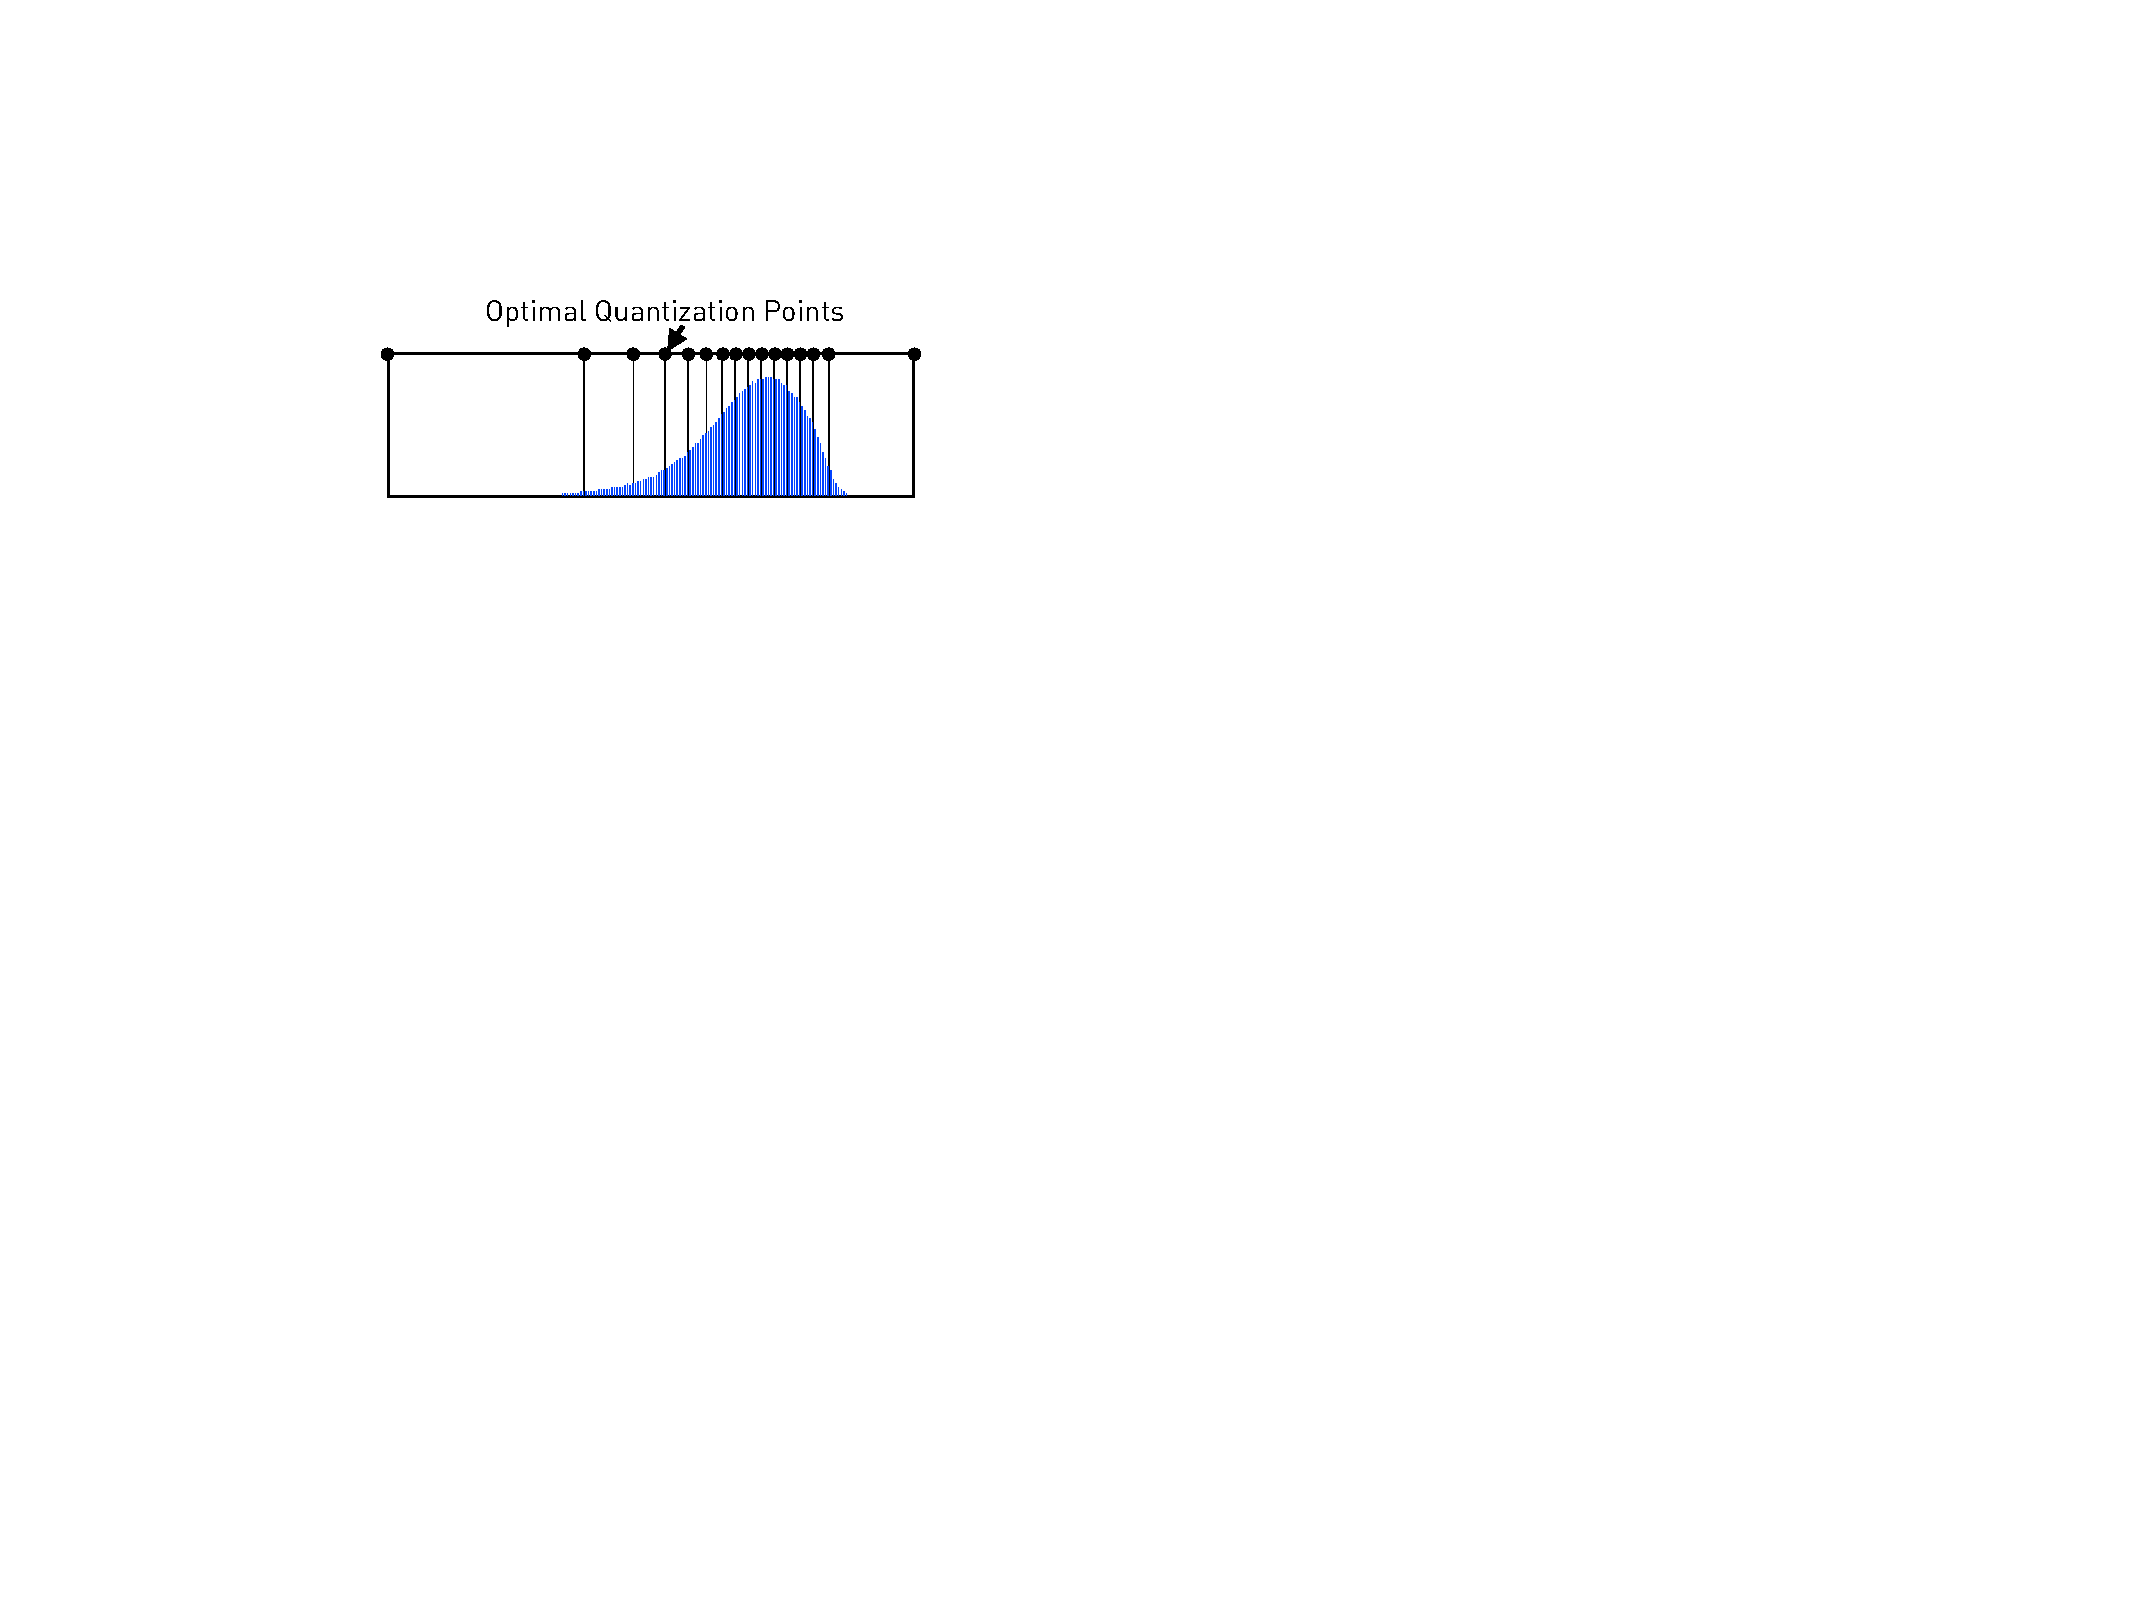
\includegraphics[width=0.5\columnwidth]{micro-experiments/dp-level.pdf} 
\vspace{-1em}
\caption{Optimal quantization points calculated with
dynamic programming given a data distribution. }
\vspace{-1em}
\label{fig:optimalquantization}
\end{figure} 

\vspace{-0.5em}
\subsection{Heuristics}
\vspace{-0.5em}

The exact algorithm has a complexity that is quadratic to the number of data points. To make our algorithm practical,
we develop an approximation algorithm that only needs to scan all data points once and has linear complexity to $N$.

\vspace{-0.5em}
\paragraph*{Discretization}

We can discretize the range $[0,1]$ into $M$ intervals, i.e., $[0,d_1), [d_1, d_2), \cdots, [d_{M-1}, 1]$ with $0< d_1<d_2<\cdots < d_{M-1}<1$. We then restrict our algorithms to only choose $k$ quantization points within these $M$ points, instead of all $N$ points in the exact algorithm. The following result bounded the quality of this approximation.

\begin{theorem} \label{thm:optQ}
Let the maximal number of data points in each ``small interval'' (defined by $\{d_m\}_{m=1}^{M-1}$) and the maximal length of small intervals be bounded by $bN/M$ and $a/M$, respectively. Let ${\mathcal{I}^*} := \{l^*_j\}_{k=1}^{k-1}$ and $\hat{\mathcal{I}}^* :=\{\hat{l}^*_k\}_{k=1}^{k-1}$ be the optimal quantization to \eqref{eq:opt_Q} and the solution with discretization. Let $cM/k$ be the upper bound of the number of small intervals crossed by any ``large interval'' (defined by ${\mathcal{I}}^*$). Then we have the discretization error bounded by
\vspace{-0.5em}
\[
 \mathcal{MV}(\hat{\mathcal{I}}^*) -  \mathcal{MV}({\mathcal{I}}^*) \leq {a^2b k \over 4 M^3} + {a^2bc^2 \over Mk}.
\]
\end{theorem}

\begin{proof}
Let $p^*_0$ be $0$ and $p^*_K=1$.We quantitize $\{p^*_k\}_{k=1}^{K-1}$ one element by one element, while monitor the changing of the total variance $N \times \mathcal{MV(\cdot)}$. We first quantize $p^*_1$ to the closest value (denoted it by $Q(p^*_1)$) in $\{d_m\}_{m=1}^{M-1} \cup \{p^*_0,p^*_K\}$ under the monotonicity constraint, that is, $p^*_0\leq Q(p^*_1) \leq p^*_2$. Here, one important observation is $|p^*_{1} - Q(p^*_1)|\leq a/M$. Consider the total variance of this new solution $Q(p^*_1), p^*_2, \cdots, p^*_{K-1}$. The variance of points falling into the range $[p^*_2, 1]$ does not change at all. Without the loss of generality, assume $p^*_{1} \geq Q(p^*_1)$.

Next we consider points falling into the following three sets $C_1 = [p^*_0, Q(p^*_1)]$, $C_2 = [Q(p^*_1), p^*_1]$, and $C_3 = [p^*_1, p^*_2]$. The variance of points of falling into $C_1$ gets reduced from the form of variance in \eqref{eq:var}. Next we only need to check the variance change for points in $C_2$ and $C_3$. Consider $C_2$ first. The variance for point $x$ in $C_2$ is
\[
(x-Q(p^*_1))(p^*_1 - x) \leq {a^2 \over 4 M^2}. 
\]  
Thus, the change of variance for points in $C_2$ would be bounded by ${a^2 \over 4 M^2}$. Then consider $C_3$. The change of variance for point $x$ in $C_3$ is
\begin{align*}
& (x-Q(p^*_1))(p^*_2 - x) - (x-p^*_1) (p^*_2 - x) 
\\
= & (p^*_1 - Q(p^*_1)) (p^*_2 - x)
\\
\leq & {a\over M}(p^*_2 - x)
\end{align*}
Therefore, the change of total variance from $\{p^*_1, p^*_2, \cdots, p^*_{K-1}\}$ to $\{Q(p^*_1), p^*_2, \cdots, p^*_{K-1}\}$ is bounded by 
\begin{align}
\nonumber
& \sum_{x\in C_2} {a^2 \over 4M^2} + \sum_{x \in C_3} {a\over M}(p^*_2 - x)
\\
\nonumber
\leq & {Nb \over M} {a^2 \over 4M^2} + {a\over M}{Nb \over M} \sum_{t=1}^{cM/K}t{a\over M}
\\
\leq &
{a^2b N \over 4 M^3} + {a^2bc^2 N \over MK^2}
\label{eq:bound_1step}
\end{align}
Similarly, we quantitize $p^2_2$ in $\{Q(p^*_1), p^*_2, \cdots, p^*_{K-1}\}$ to get a new solution $\{Q(p^*_1), Q(p^*_2), \cdots, p^*_{K-1}\}$ while maintain the monotonicity. We can establish the same upper bound to \eqref{eq:bound_1step}. Following this idea, we can obtain a quantization solution $\{Q(p^*_1), Q(p^*_2), \cdots, Q(p^*_{K-1})\}$. Therefore, we obtain that 
\begin{align*}
&  \mathcal{MV}(Q(p^*_1), Q(p^*_2), \cdots, Q(p^*_{K-1})) -  \mathcal{MV}({p}^*_1,\cdots, {p}^*_{K-1}) 
 \\
 & \quad \leq {a^2b K \over 4 M^3} + {a^2bc^2 \over MK}.
\end{align*}
Using the fact that $ \mathcal{MV}(p^*_1,\cdots, p^*_{K-1})$ is smaller than $\mathcal{MV}(Q(p^*_1), Q(p^*_2), \cdots, Q(p^*_{K-1}))$ proves the claim.
\end{proof}
%Here the constant $b$ roughly measures the 
%``uniformness of the data distribution w.r.t. small intervals'', and $a$ roughly measures ``the distortion 
%from equal-length small intervals'' (more details in 
%the full version). 
%Similarly, $c$ roughly measures the distortion from equal-length large intervals since $c=1$ means that all large intervals defined by $\{l^*_k\}_{k=1}^{s-1}$ roughly cross the same number of small intervals defined by $\{d_m\}_{m=1}^{M-1}$. 
\vspace{-0.5em}
Theorem~\ref{thm:optQ} suggests that the mean variance using the discrete variance-optimal quantization will converge to the optimal with the rate $O(1/Mk)$.

\vspace{-0.5em}
\paragraph*{Dynamic Programming with Candidate Points}
Notice that we can apply the same dynamic programming approach given $M$ candidate points. 
In this case, the total computational complexity becomes $O((k+1)M^2 + N)$, with memory cost 
$O(kM + M^2)$. Also, to find the optimal quantization,  we only need to scan all $N$ numbers once.
Figure~\ref{fig:optimalquantization} illustrates an example output for our algorithm.



%%%%


%Moreover, to get the output of the algorithm down to size exactly $k$, we may also do an additional dynamic programming postprocessing routine on the output of this algorithm.
%This postprocessing now looks for the best partition with $s$ pieces at endpoints given by endpoints of $\setI$, and so runs in time $O(k^2 N)$, i.e., nearly-linear in the number of samples.


%The goal is to find  
%the optimal set of $s$ quantization 
%levels $\{l_1, l_2, \cdots, l_{s-1}\}$ 
%which minimize the mean quantization variance. Formally:
%\begin{align}
%\nonumber \min_{l_1, \cdots, l_{s-1}} \quad & \mathcal{MV}(l_1,\cdots, l_{s-1}) := {1\over N}\sum_{x\in \Omega} \sum_{k=1}^s {\bf 1}_k(x)V_k(x)\\
%\text{s.t.}\quad & 0 = l_0 \leq l_1\leq l_2 \leq \cdots \leq l_{s-1} \leq l_s = 1.
%\label{eq:opt_Q}
%\end{align}
%where ${\bf 1}_k(x)$ is the indicator function
%\[
%{\bf 1}_k(x) = 
%\begin{cases}
%1 & \text{if}~x\in (l_{k-1}, l_k] \\
%0 & \text{o.w.}
%\end{cases}
%\]
%and $V_k(x)$ is the variance function 
%\begin{align}
%V_k(x) = (x-p_{k-1})(p_k - x), \label{eq:var}
%\end{align}
%which is the variance of Bernoulli distribution with probability $l_k-x$ taking value $l_{k-1}$ and probability $x-l_{k-1}$ taking value $l_k$. ${\bf 1}_k(x)V_k(x)$ is the variance if $x$ falls into the interval $(l_{k-1}, l_k]$. 

%This problem is hard to solve directly, due to non-convexity and non-smoothness. We discretize the range $[0,1]$ into $M$ intervals, i.e., $[0,d_1), [d_1, d_2), \cdots, [d_{M-1}, 1]$ with $0< d_1<d_2<\cdots < d_{M-1}<1$. All $l_k$'s are restricted to values in $\{d_1, d_2, \cdots, d_{M-1}\}$ while satisfying  monotonicity. 
%
%\begin{theorem} \label{thm:optQ}
%Let the maximal number of data points in each ``small interval'' (defined by $\{d_m\}_{m=1}^{M-1}$) and the maximal length of small intervals be bounded by $bN/M$ and $a/M$, respectively. Let $\{l^*_k\}_{k=1}^{s-1}$ and $\{\hat{l}^*_k\}_{k=1}^{s-1}$ be the optimal quantization to \eqref{eq:opt_Q} and the solution with discretization. Let $cM/s$ be the upper bound of the number of small intervals crossed by any ``large interval'' (defined by $\{l^*_k\}_{k=1}^{s-1}$). Then we have the discretization error bounded by
%\[
% \mathcal{MV}(\hat{l}^*_1,\cdots, \hat{l}^*_{s-1}) -  \mathcal{MV}(l^*_1,\cdots, l^*_{s-1}) \leq {a^2b s \over 4 M^3} + {a^2bc^2 \over Ms}.
%\]
%\end{theorem}
%
%Note that if the numbers of data points falling into all small intervals are equal, then
%the constant $b$ is $1$. So $b$ roughly measures the uniformness of the data distribution w.r.t. small intervals. If all small intervals have equal length, then $a$ is equal to $1$. So $a$ roughly measures the distortion from equal-length small intervals. 
%Similarly, $c$ roughly measures the distortion from equal-length large intervals since $c=1$ means that all large intervals defined by $\{l^*_k\}_{k=1}^{s-1}$ roughly cross the same number of small intervals defined by $\{d_m\}_{m=1}^{M-1}$. Theorem~\ref{thm:optQ} suggests that the mean variance using the discrete variance-optimal quantization will converge to the optimal with the rate $O(1/Ms)$.




%\paragraph*{Approximate dynamic programming}
%This program requires quadratic time in $N$ to run, which is often infeasible in practice.
% We discretize the range $[0,1]$ into $M$ intervals, i.e., $[0,d_1), [d_1, d_2), \cdots, [d_{M-1}, 1]$ with $0< d_1<d_2<\cdots < d_{M-1}<1$. All $l_k$'s are restricted to values in $\{d_1, d_2, \cdots, d_{M-1}\}$ while satisfying  monotonicity. 
%
%\begin{theorem} \label{thm:optQ}
%Let the maximal number of data points in each ``small interval'' (defined by $\{d_m\}_{m=1}^{M-1}$) and the maximal length of small intervals be bounded by $bN/M$ and $a/M$, respectively. Let $\{l^*_k\}_{k=1}^{s-1}$ and $\{\hat{l}^*_k\}_{k=1}^{s-1}$ be the optimal quantization to \eqref{eq:opt_Q} and the solution with discretization. Let $cM/s$ be the upper bound of the number of small intervals crossed by any ``large interval'' (defined by $\{l^*_k\}_{k=1}^{s-1}$). Then we have the discretization error bounded by
%\[
% \mathcal{MV}(\hat{l}^*_1,\cdots, \hat{l}^*_{s-1}) -  \mathcal{MV}(l^*_1,\cdots, l^*_{s-1}) \leq {a^2b s \over 4 M^3} + {a^2bc^2 \over Ms}.
%\]
%\end{theorem}
%

%where $V(j,m)$ denotes the total variance of points falling into the interval $[d_j, d_m]$. 
%The optimal value for $l_{s-1}^*$ is $ d_{j^*_{s-1}}$ with $j^*_{s-1}$ equal to
%\[
%j^*_{s-1} = \argmin_{j\in \{s-1, k, \cdots, M-1\}} T(s-1,j) + V(j,M),
%\]
%and the rest can be retrieved by 
%\begin{align*}
%j^*_{k-1} = \argmin_{j\in \{k-1, k, \cdots, j^*_k-1\}} T(k-1, j) + V(j, j^*_k) \\
%\text{for all}~k=2, \cdots, K-2
%\end{align*}

%The complexity of calculating the matrix $V(\cdot, \cdot)$ is $O(M^2 + N)$ and the complexity of calculating matrix $T(\cdot, \cdot)$ is $O(sM^2)$. The total memory cost is $O(sM + M^2)$. Note that to find the optimal quantization, we only need to scan all $N$ numbers once.
%The calculation of $V$ is not trivial (it needs
%another dynamic programming algorithm) and we
%describe the details in the full version.

%Define $T(k, m)$ be the optimal total variance for points in $[0, d_m]$ with $k$ quantization levels. Our goal is to calculate $T(s, M)$. This problem can be solved by dynamic programing using the following recursion
%\[
%T(k, m) = \min_{j\in \{k-1, k, \cdots, m-1\}} T(k-1,j) + V(j,m),
%\]
%where $V(j,m)$ denotes the total variance of points falling into the interval $[d_j, d_m]$. The optimal value for $l_{s-1}^*$ is $ d_{j^*_{s-1}}$ with $j^*_{s-1}$ equal to
%\[
%j^*_{s-1} = \argmin_{j\in \{s-1, k, \cdots, M-1\}} T(s-1,j) + V(j,M),
%\]
%and the rest can be retrieved by 
%\begin{align*}
%j^*_{k-1} = \argmin_{j\in \{k-1, k, \cdots, j^*_k-1\}} T(k-1, j) + V(j, j^*_k) \\
%\text{for all}~k=2, \cdots, K-2
%\end{align*}
%
%The complexity of calculating the matrix $V(\cdot, \cdot)$ is $O(M^2 + N)$ and the complexity of calculating matrix $T(\cdot, \cdot)$ is $O(sM^2)$. The total memory cost is $O(sM + M^2)$. Note that to find the optimal quantization, we only need to scan all $N$ numbers once.
%The calculation of $V$ is not trivial (it needs
%another dynamic programming algorithm) and we
%describe the details in the full version.
%Figure~\ref{fig:optimalquantization} illlustrates
%an example output for our algorithm.




%We require the following lemma, whose proof is trivial and omitted.
%\begin{lemma}
%If $I \subseteq I'$, then $\err(\setX, I) = \err (\setX_I, I) \leq \err (\setX_I, I')$.
%\end{lemma}

\section{A Greedy Algorithm for Finding Quantization Points}
\subsection{Setup}
We have $n$ points $\setX = x_1, \ldots, x_n \in [0, 1]$.
Our goal is to partition $[0, 1]$ into $k$ intervals $I_1, \ldots, I_k$, so that if we quantize all $x_i$ in $I_j$ to an endpoint of $I_j$, we minimize the variance.
If $I = [a, b]$, and $x \in I$, it is not hard to show that the variance of the quantization is given by $\err (x, I) = (b - x) (x - a)$.

\paragraph{Notation} Given an interval $I \subseteq [0, 1]$, we let $\setX_I$ be the set of $x_j \in \setX$ contained in $I$.
We also define $\err (\setX, I) = \sum_{x_j \in I} \err (x_j, I)$.
Given a partition $\setI$ of $[0, 1]$, we let $\err (\setX, \setI) = \sum_{I \in \setI} \err (\setX, I)$.
We also let $\setI^* = \argmin_{|\setI| = k} \err (\setX, \setI)$ (if there are multiple, then choose one arbitrarily), and we let $\OPT_k = \err(\setX, \setI^*)$.

We require the following lemma, whose proof is trivial and omitted.
\begin{lemma}
\label{lem:subset}
If $I \subseteq I'$, then $\err(\setX, I) = \err (\setX_I, I) \leq \err (\setX_I, I')$.
\end{lemma}

\subsection{A nearly linear time algorithm for nearly minimizing the error}
First, we observe that it is trivial that the optimal partition must have endpoints solely at points in $\setX$.
Thus we may restrict our attention to such partitions.
The algorithm is given in Algorithm \ref{alg:adaquant}.
The algorithm is inspired by  greedy merging algorithms for histogram recovery.

\begin{algorithm}[htb]
\begin{algorithmic}[1]
\Function{AdaQuant}{$\setX, k, \gamma, \delta$}
\State Let $\setI = [0, 1]$ be a partition of $[n]$, initially with one breakpoint at each point in $\setX \cup \{0, 1\}$.
\While{$|\setI| > 2(1 + \gamma) k + \delta$}
    \State Pair up consecutive intervals in $\setI$ to form $\setJ$
    \For{each $I \in \setJ$}
        \State Let $e_I = \err (\setX, I)$
    \EndFor
    \State Let $\setJ_1$ be the set of $(1 + \gamma) k$ intervals $I \in \setI$ with largest $e_I$.
    \For{each $I \in \setJ_1$}
        \State Let $I = I_1 \cup I_2$, where $I_1, I_2 \in \setI$
        \State Remove $I$ from $\setJ$
        \State Insert $I_1, I_2$ into $\setJ$
    \EndFor
    \State Let $\setI \gets \setJ$
\EndWhile
\State \textbf{return} the partition with endpoints at $\setI$.
\EndFunction
\end{algorithmic}
\caption{Nearly-linear time algorithm for finding quantization points}
\label{alg:adaquant}
\end{algorithm}

We first show this algorithm runs in nearly linear time:
\begin{theorem}
Given any $\setX, k, \gamma, \delta$, we have that $\textsc{AdaQuant} (\setX, k, \gamma, \delta)$ runs in time $O(n (\log (n / \gamma) + \log \log 1 / \delta))$ 
\end{theorem}


Our main contribution is to show that the algorithm does indeed achieve good error:
\begin{theorem}
Given any $\setX, k, \gamma, \delta$, let $\setI$ be the output of $\textsc{AdaQuant} (\setX, k, \gamma, \delta)$.
Then we have that $\err (\setX, \setI) \leq \left( 1 + \frac{1}{\gamma} \right) \OPT_k$.
\end{theorem}
\begin{proof}
Partition $\setI = \setF \cup \setJ$, where $\setF$ is the set of intervals $I \in \setI$ so that $I \subseteq I'$ for some $I' \in \setI^*$, and let $\setJ$ be the remaining intervals.
Observe that by a simple counting argument, we have that $|\setJ| \leq k$.
By Lemma \ref{lem:subset}, we have that 
\[
\sum_{I \in \setF} \err(\setX, I) \leq \OPT_k \; .
\]
We now seek to bound the error along intervals in $\setJ$.
Let $I \in \setJ$.
It must have been merged in some iteration of \textsc{AdaQuant}.
Therefore, in that iteration, there must have been $(1 + \gamma)k$ merged intervals $J_1, \ldots, J_{(1 + \gamma) k}$ so that $\err (\setX, I) \leq \err (\setX, J_\ell)$, for all $\ell = 1, \ldots, (1 + \gamma) k$.
By a simple counting argument, at most $k$ of the $J_\ell$ are not contained in some interval in $\setI^*$.
WLOG, assume that $J_1, \ldots, J_{\gamma \ell}$ are all contained in some interval of $\setI^*$.
By Lemma \ref{lem:subset}, we have that $\sum_{j = 1}^{\gamma \ell} \err (\setX, J_j) \leq \OPT$.
In particular, this implies that $\err (\setX, I) \leq \OPT / (\gamma k)$.
Since this holds for all $I \in \setJ$, and $|\setJ| \leq k$, this implies that 
\[
\sum_{I \in \setJ} \err (\setX, I) \leq k \frac{\OPT_k}{\gamma k} \leq \frac{1}{\gamma} \OPT_k \; .
\]
Combining the above two expressions yields that $\err (\setX, \setI) \leq  \left( 1 + \frac{1}{\gamma} \right) \OPT_k$, as claimed.
\end{proof}

\section{Implementation on FPGA}
\label{section:implementation}
%We describe the FPGA implementations. First, we introduce the target platform, Intel Xeon+FPGA. Then, we present our FPGA implementations for SGD that work on 32-bit floating point data and lower precision quantized data, respectively. Under each subsection, we discuss the trade-off for the circuit design we faced during the implementation phase.
In this section, we show the computation pipeline for full-precision SGD and quantized SGD implemented on FPGA in figure~\ref{fig:floatFPGASGD} and~\ref{fig:qallFPGASGD}. The FPGA implementation work is submitted to IEEE International Symposium on Field-Programmable Custom Computing Machines (FCCM) 2017.

First, we introduce the target platform, Intel Xeon+FPGA. Then, we present our FPGA implementations for SGD that work on 32-bit floating point data and lower precision quantized data, respectively. Under each subsection, we discuss the trade-off for the circuit design we faced during the implementation phase.

\subsection{Target platform: Intel Xeon+FPGA}
\label{section:xeonfpga}

Our target platform is the Intel Xeon+FPGA represented in Figure \ref{fig:xeonfpga}, made available through the \textit{Intel-Altera Heterogeneous Architecture Research Platform}\footnote{Following the Intel legal guidelines on publishing performance numbers we want to make the reader aware that results in this publication were generated using preproduction hardware and software, and may not reflect the performance of production or future systems.}. It combines a 10-core CPU (Intel Xeon E5-2680 v2, 2.8 GHz) and an FPGA (Altera Stratix V 5SGXEA) on a 2-socket motherboard. The FPGA has cache-coherent access to the CPU-connected main memory through QPI (Quick Path Interconnect) with a combined read and write bandwidth of around 6.5 GB/s. The usage of an FPGA accelerator, that we implement using VHDL, is pretty straightforward with Intel-provided software libraries, a QPI endpoint and an FPGA based page table of our own implementation: At the start of an application the required amount of shared memory is allocated by software in 4MB pages and the page table on the FPGA is populated with corresponding addresses. The accelerator can request cache-line wide (64B) reads and writes to the entire memory through the use of the page table and the QPI endpoint, which in addition to handling the QPI protocol also implements an FPGA local cache (128KB two-way associative) using BRAMs. Apart from the page-table, a further addition we made to the interface is a reorder buffer, since by default QPI requests arrive out of order. In addition to an accelerator requesting data from QPI, the software can also issue direct writes, a useful feature for configuring some registers containing runtime parameters.

\begin{figure}[t]
\centering
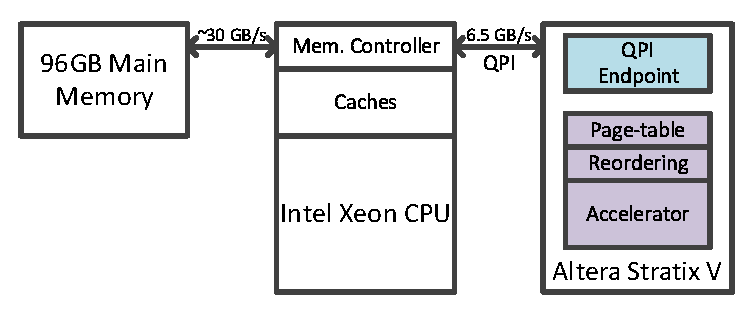
\includegraphics[width=.7\columnwidth]{Figures/XeonFPGA.eps}
\caption{Intel Xeon+FPGA Architecture}
\label{fig:xeonfpga}
\end{figure}

\subsection{FPGA-SGD on \textbf{float} data}
\label{section:floatfpgasgd}

We first present an SGD implementation on the FPGA, that works on 32-bit floating-point data, which is very often the original data representation in machine learning data sets. In Figure \ref{fig:floatFPGASGD} the computation pipeline for \textit{float} FPGA-SGD is presented. As the data access width is a 64B cache-line on Xeon+FPGA, the circuit is designed to work on that data width. It is able to accept a cache-line at every clock cycle ($f_{clock} = 200 MHz$), resulting in an internal processing rate of 12.8 GB/s.

\begin{figure}[t]
\centering
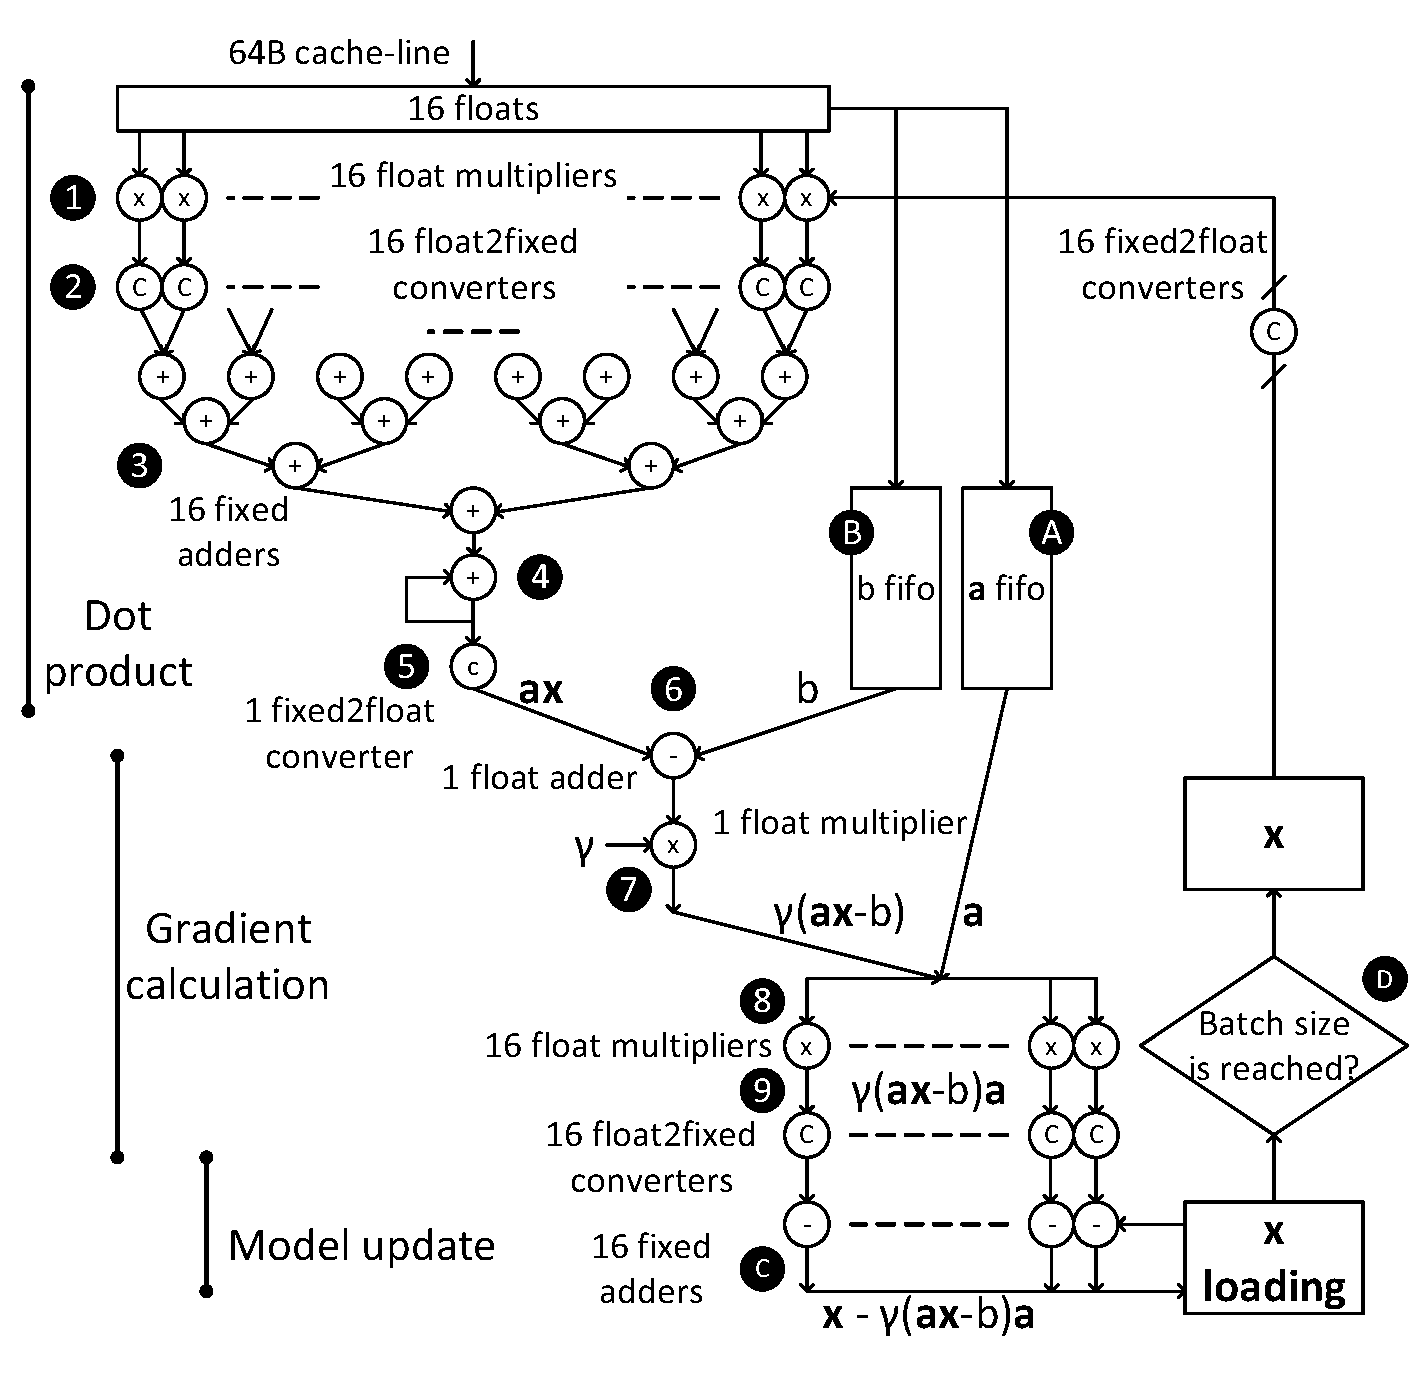
\includegraphics[width=.8\columnwidth]{Figures/floatFPGASGD.eps}
\caption{Computation pipeline for \textit{float} FPGA-SGD, with a latency of 36 cycles, a data width of 64B and a processing rate of 64B/cycle.}
\label{fig:floatFPGASGD}
\end{figure}

\noindent
\textbf{Scale to \# features:} The challenging part of the design is to make it capable of handling a number of features $D$ that is larger than 16, which is the default width of the pipeline. In fact, this is possible since all vector algebra can be performed iteratively, where each chunk contains 16 values. This implies that the number $D$ needs to be a multiple of 16. To ensure that, we use zero-padding on a data set, if $D\bmod16\neq0$. Thus, we can calculate how many cache-lines it takes for $\mathbf{a_i}$ (one row in the set) to be completely received:
\[
\text{\#} \mathbf{a_i} \text{cache-lines} = 
\begin{cases}
%\frac{D}{16}
D/16
\quad & \text{if } D\bmod16=0 \\
\frac{D + (16-D\bmod16)}{16}
%(D + (16-D\bmod16))/16
\quad & \text{if } D\bmod16\neq0
\end{cases}
\]
The only parameter that the design needs to scale for is the maximum number of dimensions $D_{max}$ that can be supported, and the only value growing with that is the amount of BRAM for storing the model $\mathbf{x}$. We choose $D_{max}$ to be 8192, since this is more than enough for most existing linear dense model training examples. The design can handle any number of samples, \textit{N}, since training is done in a streaming fashion, as explained in the following.
%The resource consumption numbers on the target FPGA are given in Table \ref{table:resources}.

\begin{figure*}[t]
\centering
\begin{subfigure}[t]{.6\columnwidth}
\centering
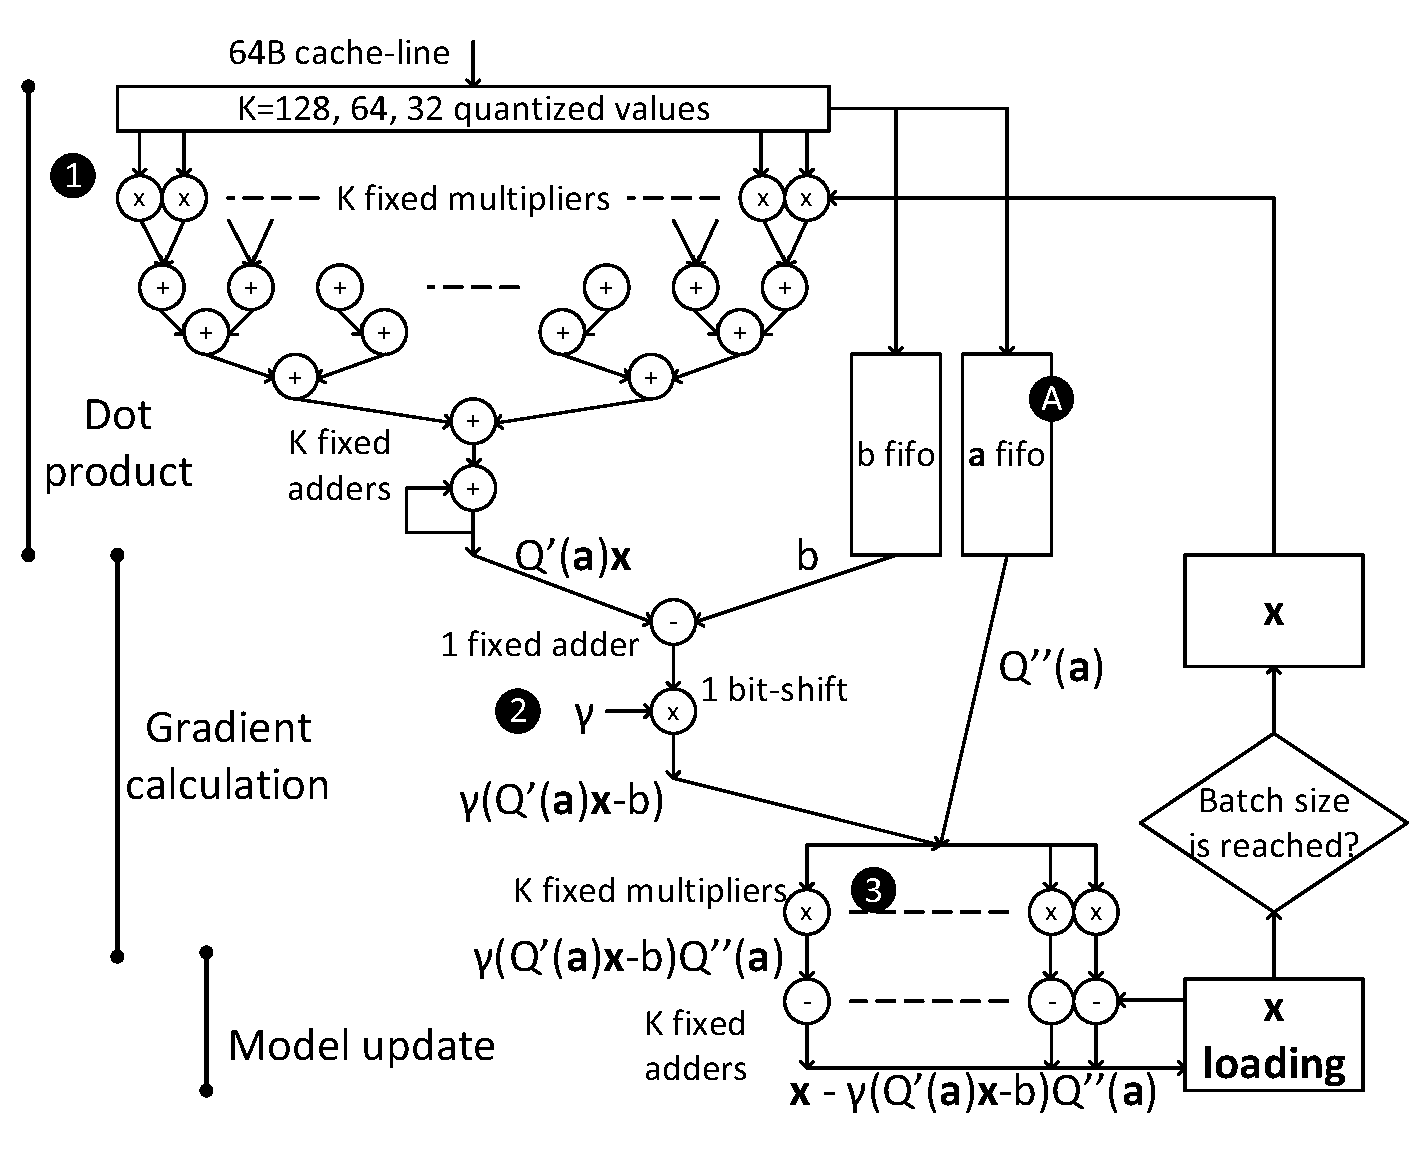
\includegraphics[width=\columnwidth]{Figures/qFPGASGD.eps}
\caption{\textit{Q2}, \textit{Q4} and \textit{Q8} FPGA-SGD, with a latency of $log(K)$+5 cycles, a data width of 64B and a processing rate of 64B/cycle.}
\label{fig:qFPGASGD}
\end{subfigure}
\quad
\begin{subfigure}[t]{.6\columnwidth}
\centering
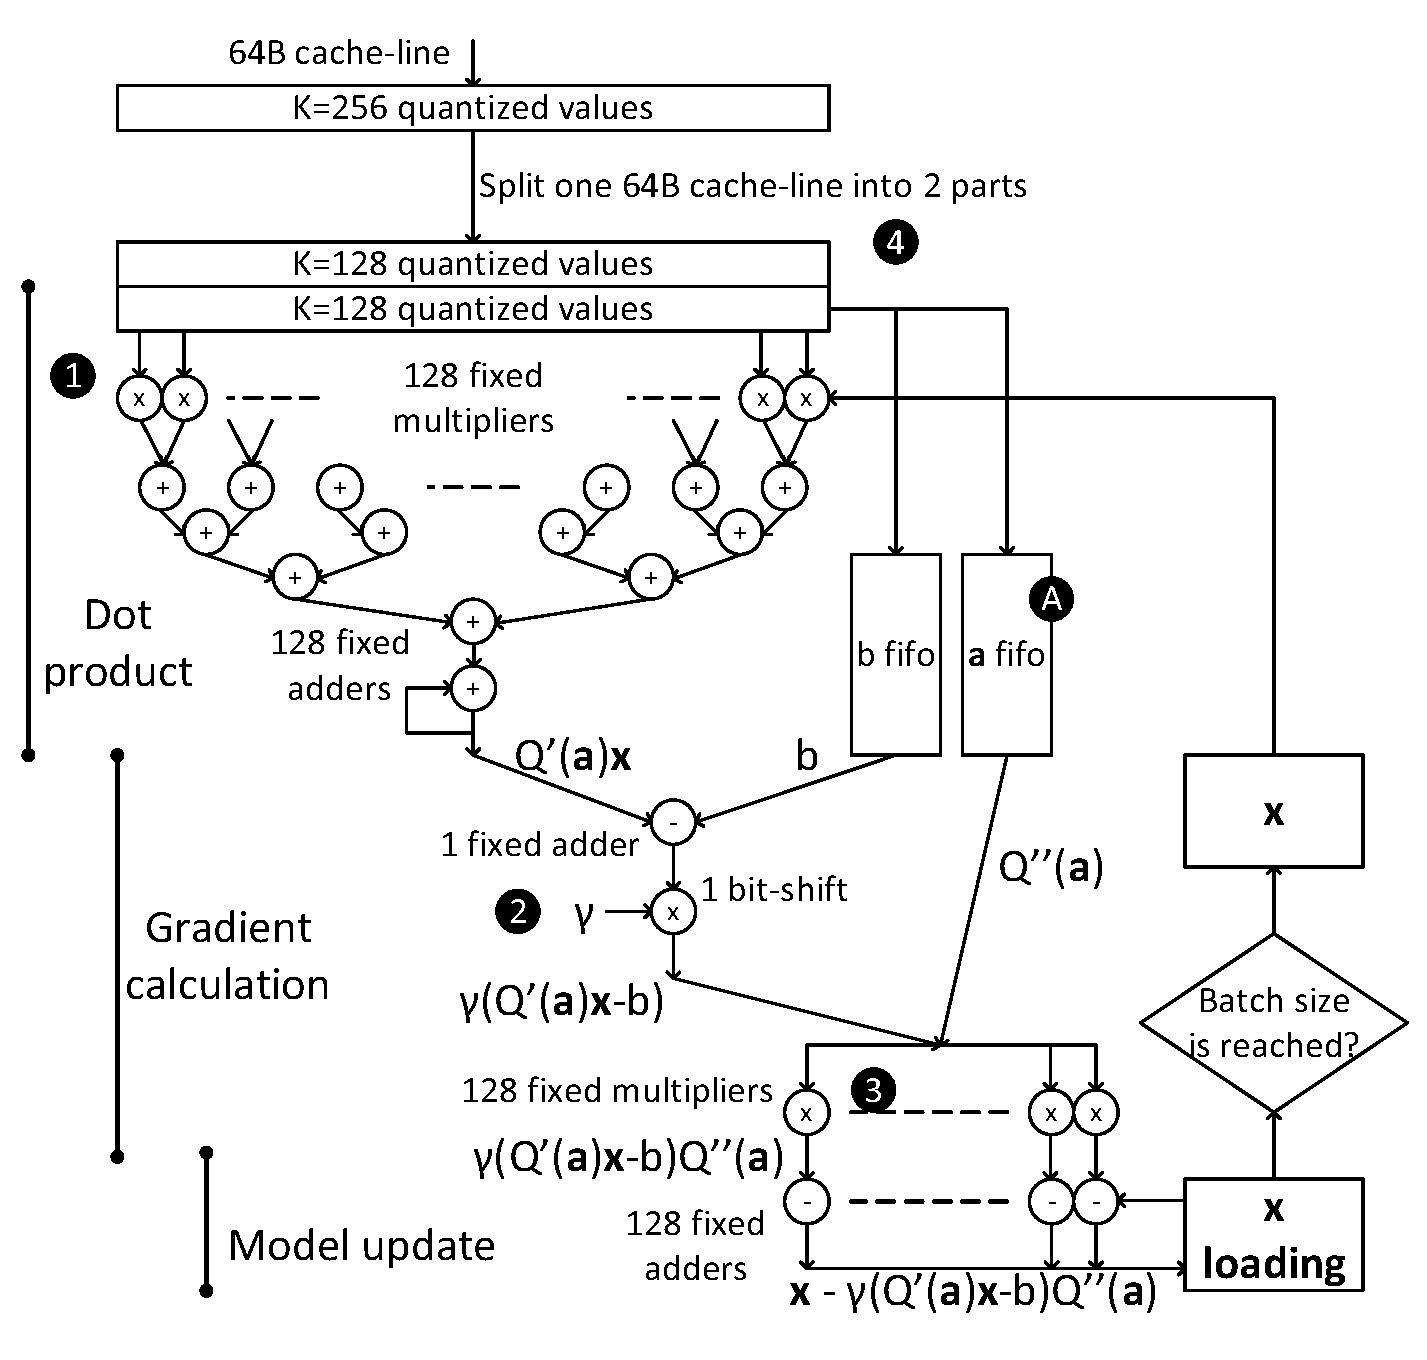
\includegraphics[width=\columnwidth]{Figures/q1FPGASGD.eps}
\caption{\textit{Q1} FPGA-SGD, with a latency of 12 cycles, a data width of 32B and a processing rate of 32B/cycle.}
\label{fig:q1FPGASGD}
\end{subfigure}
\caption{Computation pipelines for all quantizations. Although for \textit{Q2}, \textit{Q4} and \textit{Q8} the pipeline width scales out and maintains 64B width, for \textit{Q1} it does not scale out and the pipeline width needs to be halved, making \textit{Q1} FPGA-SGD compute bound.}
\label{fig:qallFPGASGD}
\end{figure*}


\noindent
\textbf{Walk-through of computation pipeline:} In the following, we explain what happens at each stage of the computation pipeline. The first stage is the dot product $\mathbf{a_i}\cdot\mathbf{x} = \sum_{j=1}^{D} a_{i,j}x_j$. When a cache-line containing a part of vector $\mathbf{a_i}$ arrives, it is first multiplied (\circled{1}) with the corresponding part of vector $\mathbf{x}$. The multiplication is performed in floating point with multiplier IPs\footnote{All floating point IPs are created via Altera Quartus II 13.1}, which have 5 cycles latency and a result per cycle throughput. Then, the values are converted to a 32-bit integer (\circled{2}) by multiplication with a large constant that is configurable during runtime, depending on the value range or the precision that is desired to be kept. This \textit{float2fixed} conversion takes 1 cyle. After that, an adder tree (\circled{3}) accumulates 16 values, each layer taking 1 cycle. At the output of the adder tree is a single accumulator (\circled{4}). It accumulates the results coming out from the adder tree for the pre-calculated number of $\text{\#} \mathbf{a_i} \text{cache-lines}$, thus building the final value for the dot product. The dot product result is converted back to floating point (\circled{5}), since the next stages of the calculation will be performed with floating point data.
In the next part, the rest of the gradient calculation takes place. First, the scalar value $b$, which is the true inference value in the data set, is subtracted from the dot product (\circled{6}) using a floating point adder IP, which has 7 cycles latency and a result per cycle throughput. As for where the $b$ value comes from, it is actually received some cycles before the subtraction takes place and is put into a FIFO (\circled{B}), waiting there until the dot product result is ready. After the subtraction, a floating point multiplication takes place with the step size $\gamma$ (\circled{7}), which can be configured to any \textit{float} value during runtime. At the end of this step, we have a scalar value $\gamma(\mathbf{a_i}\cdot\mathbf{x}-b_i)$, which needs to be multiplied with vector $\mathbf{a_i}$. At this stage, a FIFO (\circled{A}) already contains all parts of vector $\mathbf{a_i}$, because the incoming cache-lines are written to this FIFO simultaneously as they were sent to the dot product calculation. The scalar-vector multiplication (\circled{8}) takes place in floating point, where all parts of $\mathbf{a_i}$ are multiplied with the same scalar value. This gives us the gradient $\mathbf{g_i}$ one part at a time, which undergoes \textit{float2fixed} conversion (\circled{9}), so that a cycle-by-cycle update of the model $\mathbf{x}$ (\circled{C}) can take place, which would not be possible with a floating point adder having 7 cycles latency. The part of the gradient, which is ready, is applied to the corresponding part of the model. After the last part of the gradient is subtracted from the model, the update for $\mathbf{a_i}$ (a row in the data set) is completed. After all rows go through the same calculation, one so called epoch is completed. In Figure \ref{fig:floatFPGASGD} we can see that the model we apply the updates to and the model we read for the dot product are separate. Only when a certain batch size (the number of already processed $\mathbf{a_i}$) is reached, the updated model is carried on to the actual model (\circled{D}). The reason for this is the latency introduced by the computation pipeline: In theory, the whole gradient calculation and the update to the model should be an atomic operation. However, since we would like to exploit the deep-pipelining an FPGA provides to achieve high processing throughput, we don't perform this operation atomically. Instead, we keep the actual model and the updated model separate and only carry out the accumulated update when a certain batch size is reached (called also a mini-batch SGD). The batch size is a runtime configurable parameter, which should be set to the latency of the pipeline (36 cycles) to avoid any so called stale updates.

\noindent
\textbf{Trade-off: End-to-end float vs. hybrid computation} We choose a hybrid (float+fixed) over end-to-end float computation because of the following reasons: (1) One floating point addition takes 7 cycles, resulting in a high latency adder tree (\circled{3}). Because of the increased latency (as explained previously) a larger batch-size is required to avoid staleness, which slows down the convergence rate. (2) Again, since a floating point addition takes 7 cycles, a cycle-by-cycle accumulation (\circled{7}) would not be possible, since the result of an ongoing addition is required in the next cycle. Thus, for keeping the processing rate at 64B/cycle, a hybrid design is chosen.

\subsection{FPGA-SGD on \textbf{quantized} data}
\label{section:qfpgasgd}

We explain how the FPGA-SGD design for \textit{float} data is adjusted to work on quantized data. The main purpose of this design is simple: Instead of reading \textit{float} data, where only 16 values can be fit into a cache-line, we would like to quantize the data beforehand, so that we can fit more than 16 values into a cache-line, thus utilize the available bandwidth more efficiently and gain speedup. There is one main challenge in making the FPGA-SGD work on quantized data: Scaling out the computation pipeline presented in Figure \ref{fig:floatFPGASGD}, so that it can work on more than 16 values in parallel. Before we dive in and explain how this is achieved, first we would like to give an overview of quantization options we consider and how the data layout looks like.

\noindent
\textbf{Quantization for FPGA-SGD:} When we analyze what happens when we quantize data, given a non-integer value, the quantization still might produce a non-integer value. However, floating point arithmetic induced by non-integer values are hard to implement on the FPGA, and scaling out such a design would not be possible. We would like to take advantage of the fact that we can select the quantization variables $[L,U]$ and $s$ intelligently, so that only integer values are produced. In Table \ref{table:quantization} we present choices for these values.

\begin{table}[t]
\centering
\caption{Choice of quantization levels, lower and upper bounds, so that only integer values are produced.}
\label{table:quantization}
\begin{tabular}{c|c|c|c}
Levels & Data set positive & Data set negative & Needed bits\\
\hline
s=2 & $[L,U]=[0,1]$ & N/A & 1, \textit{Q1} \\
s=3 & $[L,U]=[0,2]$ & $[L,U]=[-1,1]$ & 2, \textit{Q2} \\
s=9 & $[L,U]=[0,8]$ & $[L,U]=[-4,4]$ & 4, \textit{Q4} \\
s=129 & $[L,U]=[0,128]$ & $[L,U]=[-64,64]$ & 8, \textit{Q8}
\end{tabular}
\end{table}

After we have selected a quantization precision (one of \textit{Q1}, \textit{Q2}, \textit{Q4} or \textit{Q8}), the data set (the values in matrix $\mathbf{a}$) must be normalized to selected quantization's corresponding $[L,U]$. At this stage, the sign of the data set is considered for the normalization. For example, we choose not the normalize a negative data set into a positive interval, in order to keep existing zeros, thus we don't use \textit{Q1} for negative data sets.

\noindent
\textbf{The layout of quantized data}  For calculating a correct gradient we need 2 quantization samples of the same data point. That is, if we for example select \textit{Q8}, a quantized sample has 8 bits and we need 2 of them for calculating the gradient; the actual amount of bits we use is 16. That's why, when we perform quantization on a data set, we always create 2 samples and store them in memory next to each other. Thus, we can calculate how many quantized values can fit into one cache-line, a value we call $K$, in Table \ref{table:valuesincl}. The value $K$ dictates the amount of zero-padding we need to perform, in order to be cache-line aligned, similar to as it did for \textit{float} FPGA-SGD. Thus, the number of cache-lines required to receive one quantized row $Q(\mathbf{a_i})$ can be calculated:
\begin{equation}
\label{equation:cachelines}
\text{\#} \mathbf{a_i} \text{cache-lines} = 
\begin{cases}
%\frac{D}{16}
D/K
\quad & \text{if } D\bmod K=0 \\
\frac{D + (K-D\bmod K)}{K}
%(D + (16-D\bmod16))/16
\quad & \text{if } D\bmod K\neq0
\end{cases}
\end{equation}
\begin{table}[t]
\centering
\caption{Number of received values in a single cache-line.}
\label{table:valuesincl}
\begin{tabular}{c|c|c|c|c|c}
Data type & \textit{Q1} & \textit{Q2} & \textit{Q4} & \textit{Q8} & \textit{float}\\
\hline
Number of values in a cache-line, $K$ & 256 & 128 & 64 & 32 & 16\\
\end{tabular}
\end{table}

\begin{figure}[t]
\centering
\begin{subfigure}{.9\columnwidth}
\centering
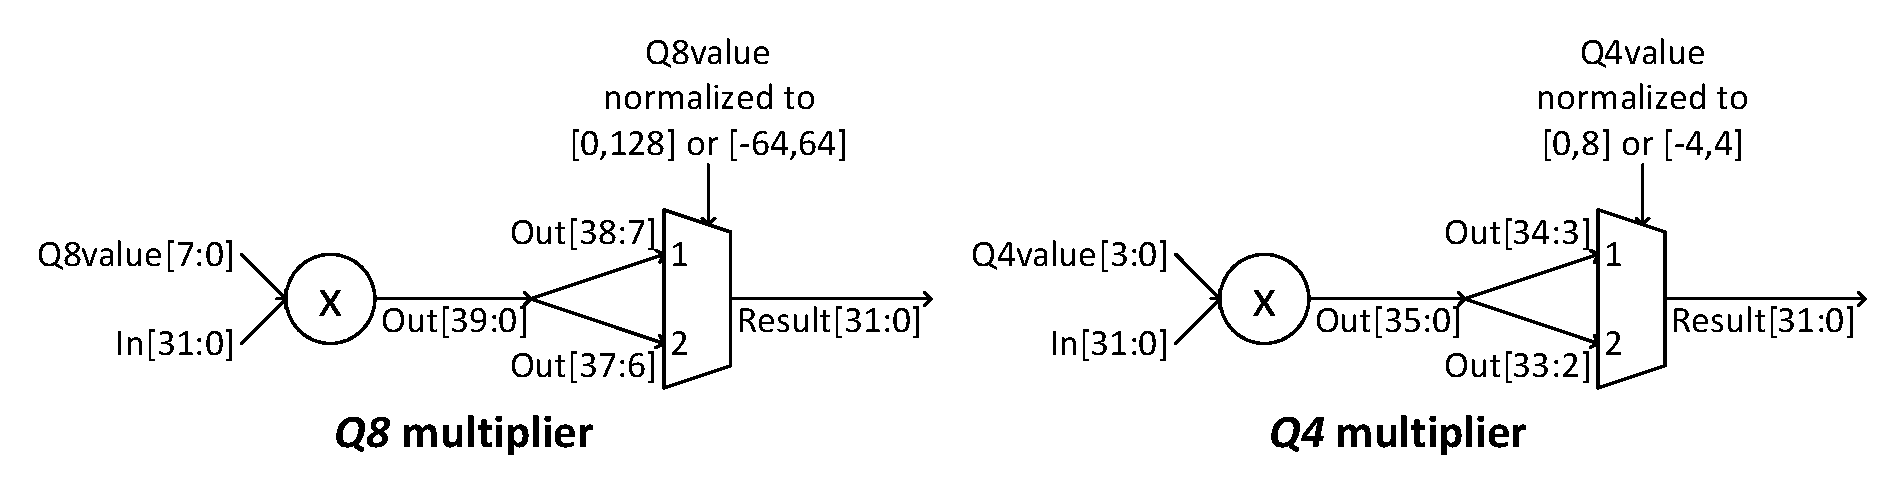
\includegraphics[width=\columnwidth]{Figures/Q8Q4mult.eps}
\caption{Signed integer multiplication for \textit{Q8} and \textit{Q4} data, implemented with DSPs.}
\label{fig:Q8Q4mult}
\end{subfigure}
\begin{subfigure}{\columnwidth}
\centering
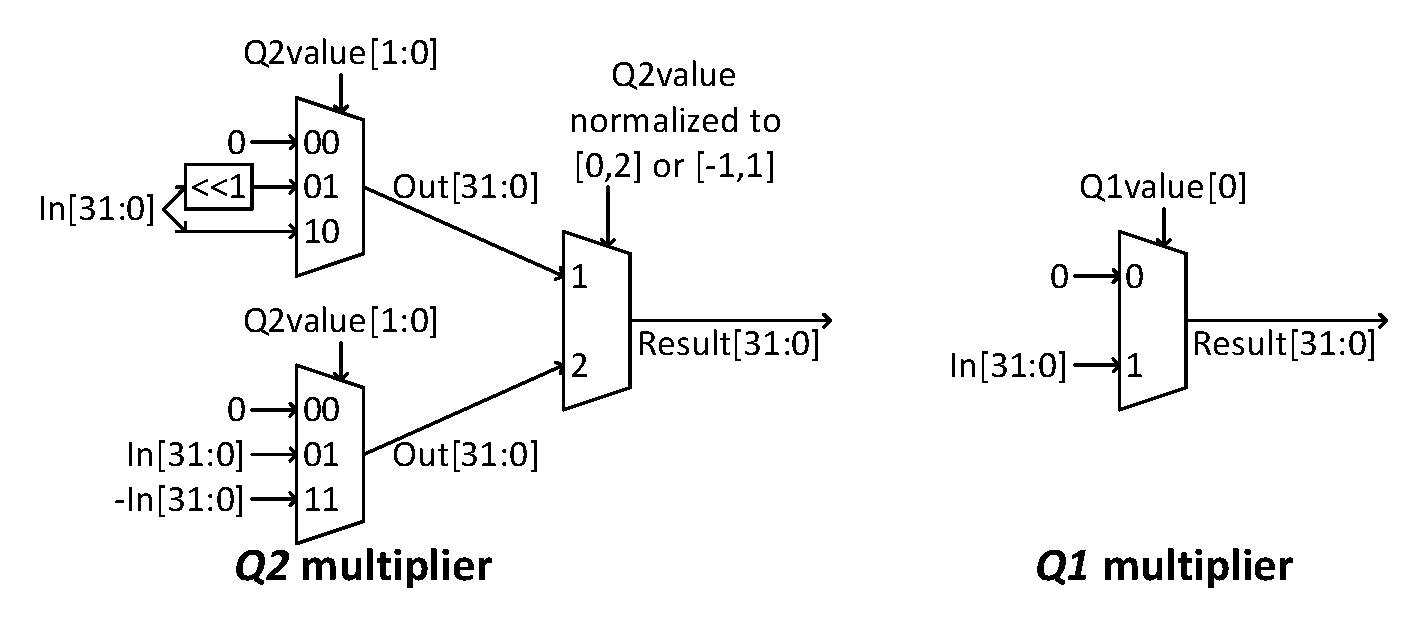
\includegraphics[width=.7\columnwidth]{Figures/Q2Q1mult.eps}
\caption{Signed integer multiplication for \textit{Q2} and \textit{Q1} data, implemented with combinational logic.}
\label{fig:Q2Q1mult}
\end{subfigure}
\caption{Multiplication implementations depending on the quantization kind.}
\label{fig:Qmult}
\end{figure}

\noindent
\textbf{Computation pipeline for quantized data:} The computation pipeline for quantized data is presented in Figure \ref{fig:qallFPGASGD}. The selection of \textit{Qx}, which determines the width of the pipeline is a generic parameter that can be set before synthesis. So, for each \textit{Qx} a different bitstream needs to be compiled. The pipeline is very similar to the \textit{float} version, explained in Section \ref{section:floatfpgasgd}. For this reason, our explanation here only focuses on the differences and how the pipelines are scaled out. The first thing to note is that \textit{Qx} pipelines are working only on integer data, so there is no need for converters. This is because, the arriving quantized data $Q(\mathbf{a_i})$ is already in integer form, as explained previously, and the inference values $b$ are also converted to integer by multiplication with a large constant. Another difference here is that for a given value in vector $\mathbf{a_i}$, 2 quantized samples arrive because of the double sampling method. The first sample is given to the dot product calculation (\circled{1}) and the second sample is put into a FIFO (\circled{A}), where it is kept until the dot product result is ready, as depicted in Figure \ref{fig:qallFPGASGD}. The last difference we would like to mention is the appliance of the step size $\gamma$ (\circled{2}), which is actually a division. Since we are dealing with integer data here, we choose to apply $\gamma$ as a bit-shift operation. By how many bits the value is shifted to right is a runtime configurable parameter, allowing adjustments according to data set characteristics.

\noindent
\textbf{Scaling out for quantized data and trade-offs:} Now, scaling out the pipeline for \textit{Q8} and \textit{Q4} is very straightforward as conventional signed multipliers (\circled{3}), implemented by DSP resources, followed by a bitshift, to keep the data width at 32 bits, is used as shown in Figure \ref{fig:Q8Q4mult}. However, for \textit{Q2} and \textit{Q1}, we can do a much more efficient multiplication using multiplexers as shown in \ref{fig:Q2Q1mult}, since one of the multiplicands is only 2 bits and 1 bit, respectively. Doing this efficient multiplication allows \textit{Q2} pipeline to scale to 128 value parallelism, which would have otherwise required a 100\% usage of the available DSP resources on the target FPGA (see Table \ref{table:resources}). However, the pipeline shown in Figure \ref{fig:qFPGASGD} does not scale to 256 value parallelism, even though \textit{Q1} multiplier is just one multiplexer. The main problem here is that the adder tree is too wide and deep, making the routing very challenging. Once it has become clear that we cannot scale the pipeline to this parallelism, we decided to halve it to process \textit{Q1} data. For doing that, we split an arriving cache-line into 2 parts (\circled{4}), which are processed sequentially by the pipeline shown in Figure \ref{fig:q1FPGASGD}. The processing rate of this pipeline is 32B/cycle, or 6.4 GB/s, which is slightly less than the memory bandwidth. Thus, \textit{Q1} FPGA-SGD will actually be compute bound.
{\tiny
\begin{table}[t]
\centering
\caption{Resource consumption for computation pipelines.}
\label{table:resources}
\begin{tabular}{c|c|c|c}
Data type & Logic (ALMs) & DSP & BRAM (bits)\\
\hline
\textit{float} & 38\% (89194) & 12\% (33) & 7\% (3.471K) \\
\textit{Q8} & 35\% (82152) & 25\% (64) & 6\% (3.145K) \\
\textit{Q4} & 36\% (84500) & 50\% (128) & 6\% (3.145K) \\
\textit{Q2}, \textit{Q1} & 43\% (100930) & 1\% (2) & 6\% (3.145K) %\\
%\textit{Q1}	& 42\% (98582) & 1\% (2) & 6\% (3.145K)
\end{tabular}
\end{table}
}





%\begin{figure}[t]
%\centering
%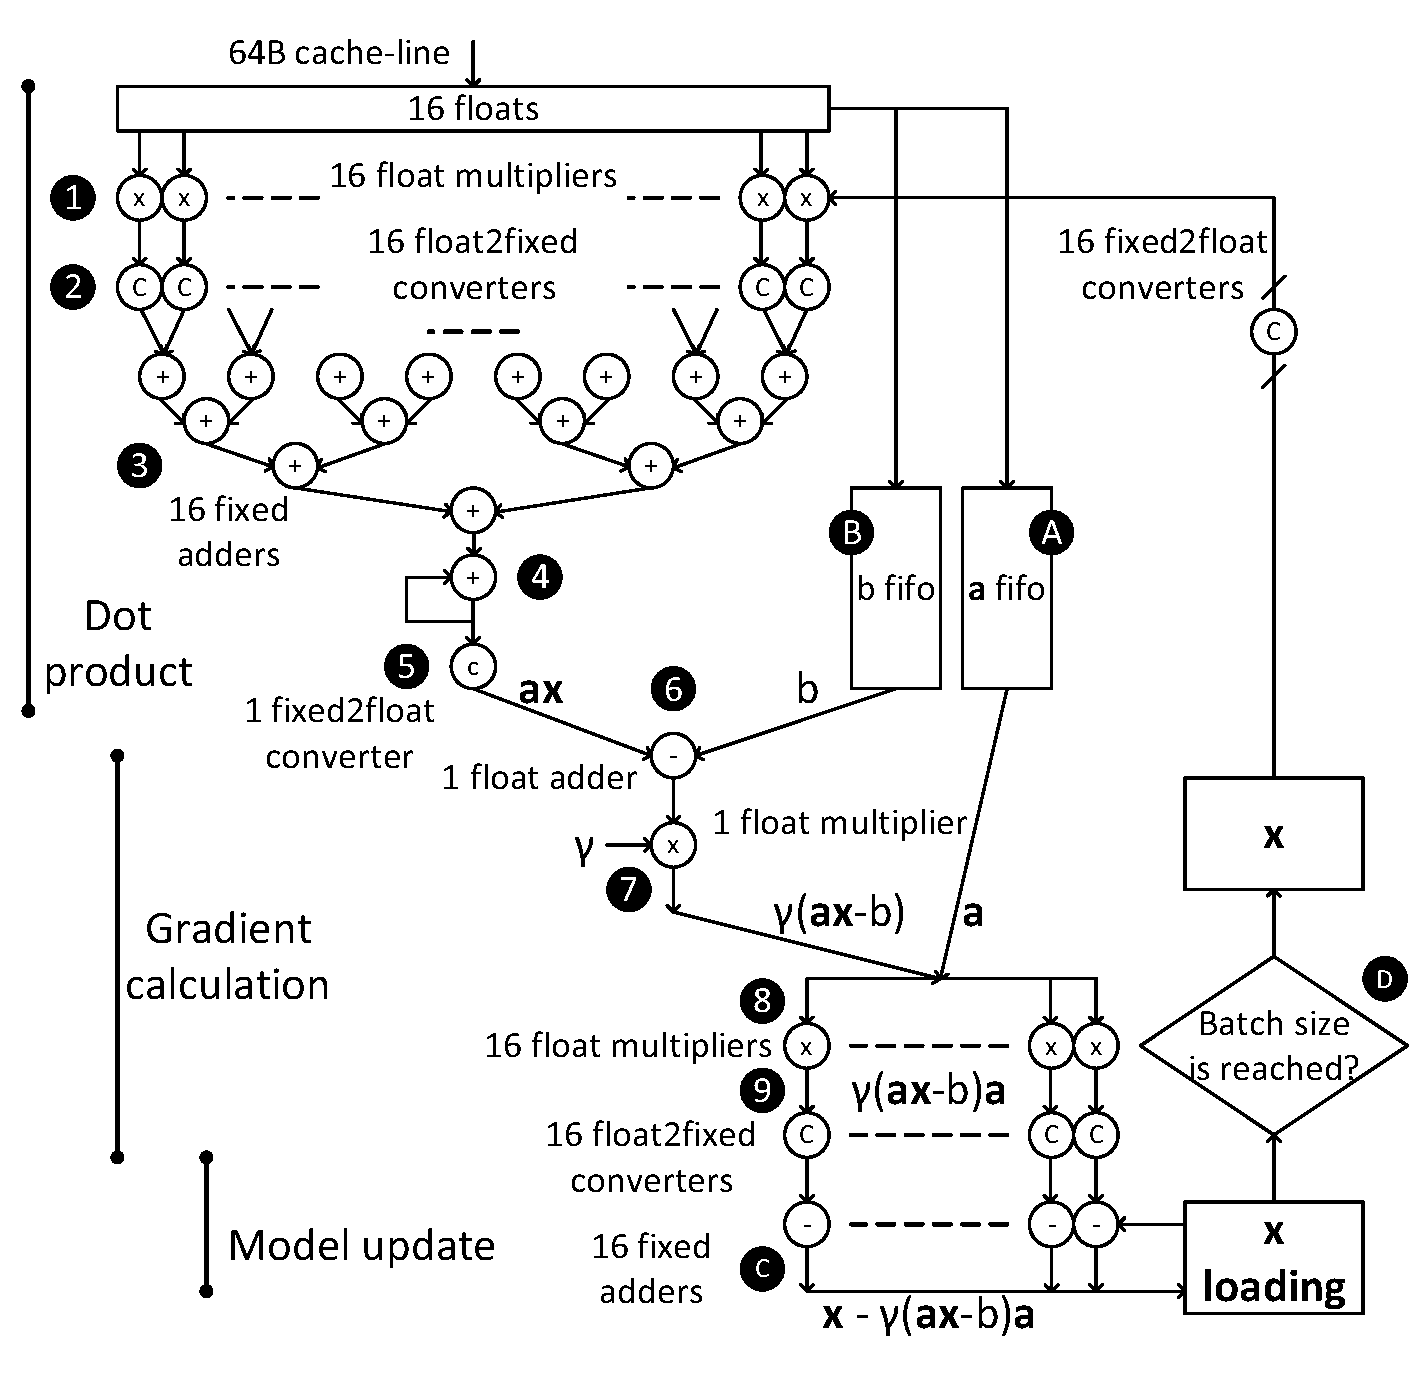
\includegraphics[width=.8\columnwidth]{Figures/floatFPGASGD.eps}
%\caption{Computation pipeline for \texttt{floatFSGD}, with a latency of 36 cycles, a data width of 64B and a processing rate of 64B/cycle.}
%\label{fig:floatFPGASGD}
%\end{figure}
%
%
%\begin{figure}[t]
%\centering
%\begin{subfigure}[t]{.8\columnwidth}
%\centering
%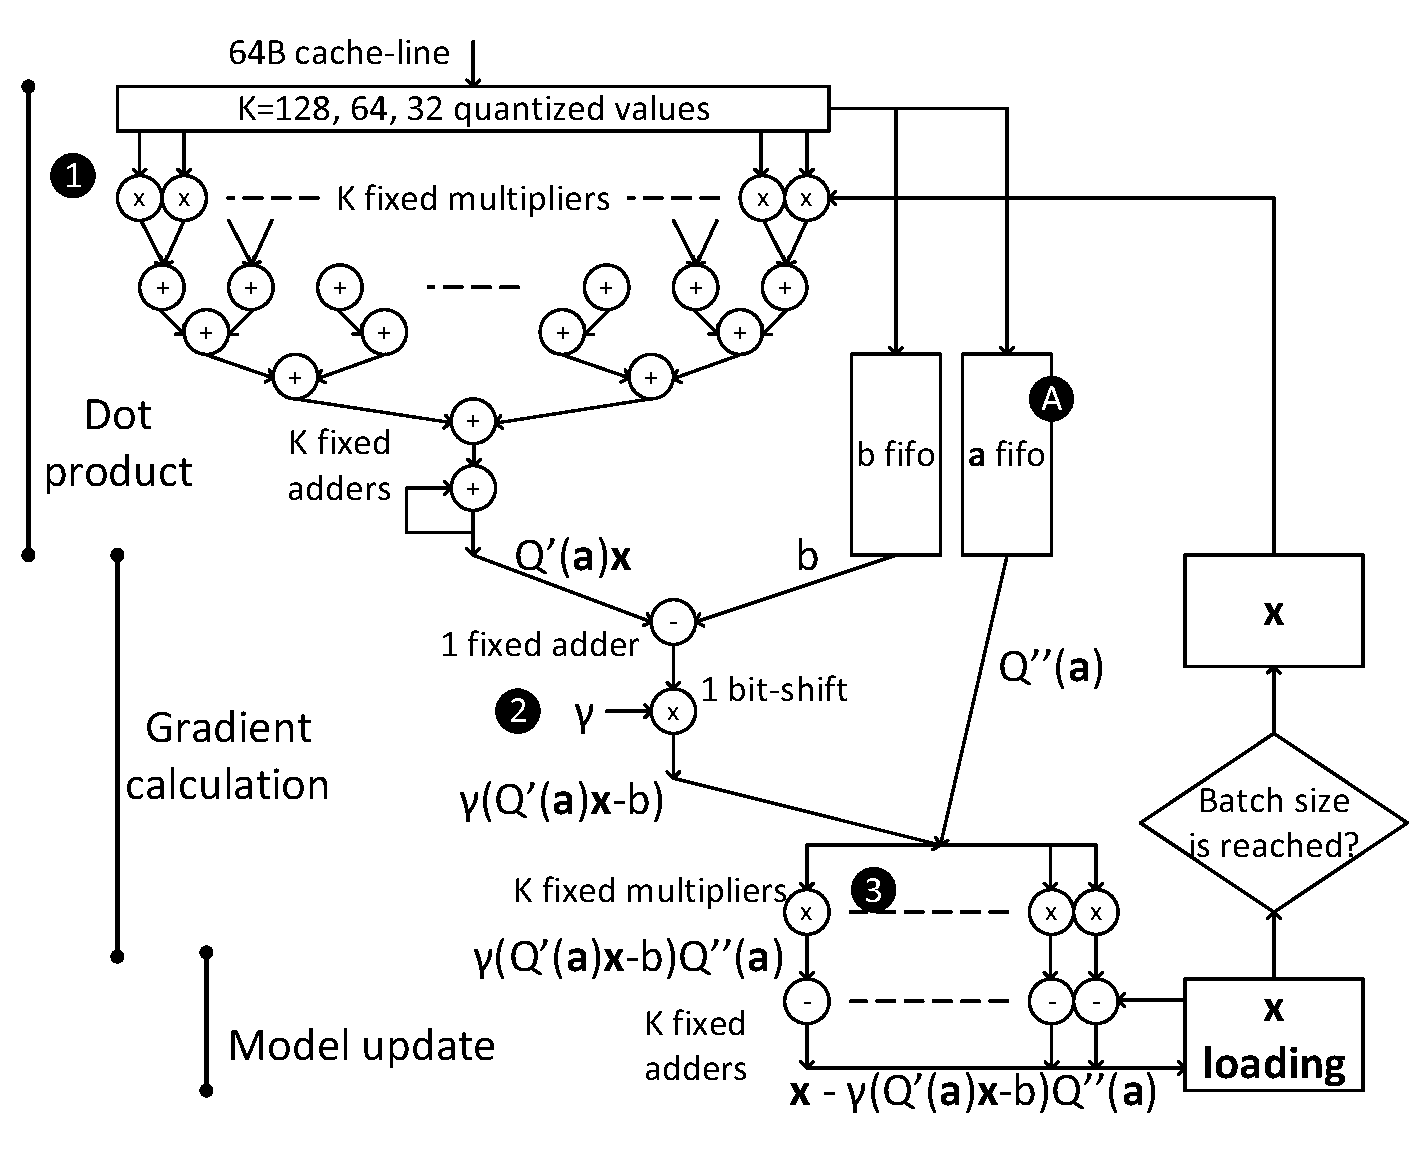
\includegraphics[width=\columnwidth]{Figures/qFPGASGD.eps}
%\caption{\textit{Q2}, \textit{Q4} and \textit{Q8} \texttt{qFSGD}, with a latency of $log(K)$+5 cycles, a data width of 64B and a processing rate of 64B/cycle.}
%\label{fig:qFPGASGD}
%\end{subfigure}
%\quad
%\begin{subfigure}[t]{.8\columnwidth}
%\centering
%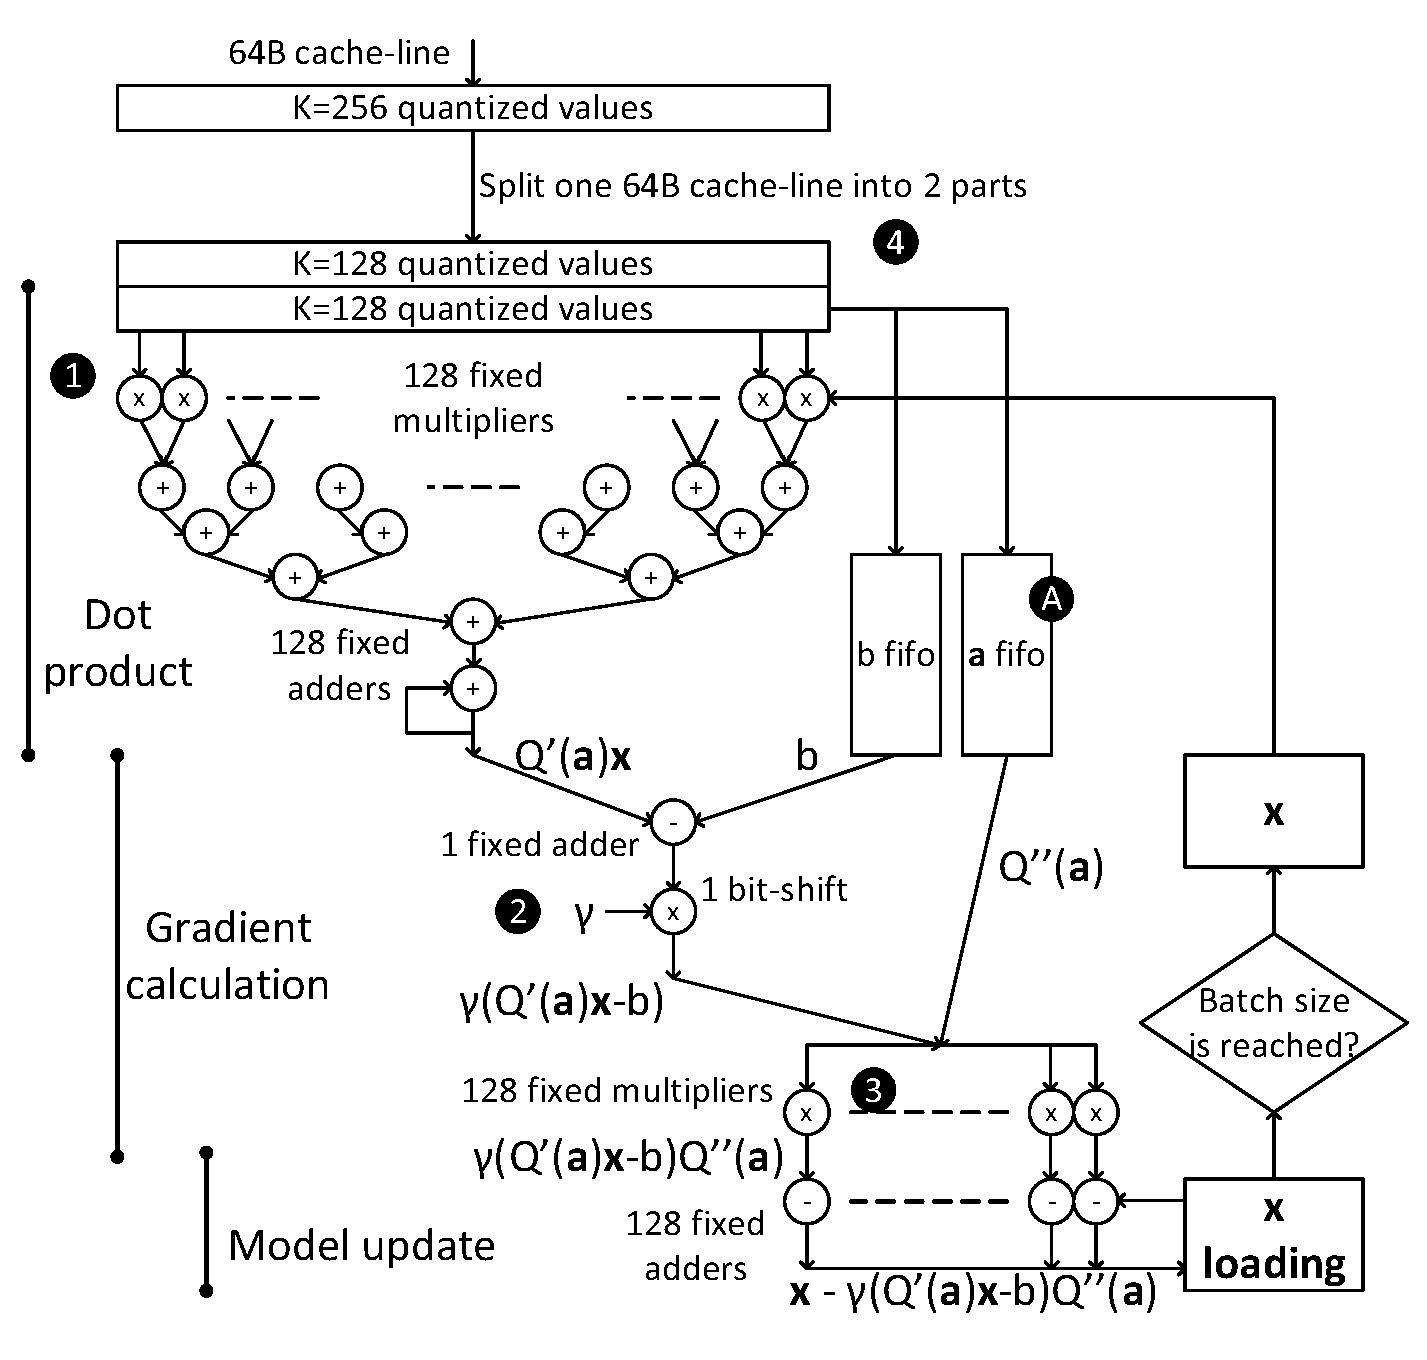
\includegraphics[width=\columnwidth]{Figures/q1FPGASGD.eps}
%\caption{\textit{Q1} \texttt{qFSGD}, with a latency of 12 cycles, a data width of 32B and a processing rate of 32B/cycle.}
%\label{fig:q1FPGASGD}
%\end{subfigure}
%\caption{Computation pipelines for all quantizations. Although for \textit{Q2}, \textit{Q4} and \textit{Q8} the pipeline width scales out and maintains 64B width, for \textit{Q1} it does not scale out and the pipeline width needs to be halved, making \textit{Q1} \texttt{qFSGD} compute bound.}
%\label{fig:qallFPGASGD}
%\vspace{-1em}
%\end{figure}



\section{Experiments}

This part is an extended version of the experiment section in the main paper.

\begin{table}[t]
\small
\centering
\begin{tabular}{crrrr}
\hline
\multicolumn{4}{c}{\bf Regression}\\
Dataset           & Training Set & Testing Set & \# Features  \\
\hline
Synthetic 10   & 10,000        & 10,000       & 10               \\
Synthetic 100  & 10,000        & 10,000       & 100              \\
Synthetic 1000 & 10,000        & 10,000       & 1,000           \\
YearPrediction & 463,715       & 51,630       & 90                  \\
cadata         & 10,000        & 10,640       & 8                   \\
cpusmall       & 6,000         & 2,192        & 12     \\
\hline
\hline
\multicolumn{4}{c}{\bf Classification}\\
Dataset           & Training Set & Testing Set & \# Features \\
\hline
cod-rna        & 59,535        & 271,617      & 8    \\
gisette        & 6,000         & 1,000        & 5,000  \\  
epsilon        & 10,000        & 10,000       & 2,000\\  
\hline
\hline
\multicolumn{4}{c}{\bf Deep Learning}\\
Dataset           & Training Set & Testing Set & \# Features \\
\hline
CIFAR-10        & 50,000        & 10,000      &$32\times 32\times 3$     \\
\hline
\hline
\multicolumn{4}{c}{\bf Tomographic Reconstruction}\\
Dataset           & \# Projections & Volumn Size & Proj. Size \\
\hline
                  & $128$            & $128\times 128\times 128$      & $128\times 128\times 128$     \\
\hline
\end{tabular}
\caption{Dataset statistics}
\label{table:dataset}
\end{table}

\paragraph{Experimental Setup} 
Table~\ref{table:dataset} shows the 
datasets we use. 
Unless otherwise noted, we always
use diminishing stepsizes $\alpha/k$,
where $k$ is the current number of
epoch. We tune 
$\alpha$ for the full precision
implementation, and use the
same initial step size for 
our low-precision 
implementation. (Theory and
experiments imply that the low-precision
implementation often favors smaller step size. 
Thus we do not tune step sizes for the low-precision 
implementation, as this can only improve the accuracy of our approach.) 

\subsection{Linear Models}

For linear models, we validate that with double sampling, SGD with low
precision converges---in comparable empirical 
convergence rates---to the same solution
as SGD with full precision.

\paragraph{Quantized Data}
We validate that (1) if we quantize data with double sampling, SGD with low precision converges---in comparable empirical 
convergence rates---to the same solution as SGD with full precision, and (2) with our optimal quantization strategy for quantizing data, we can use less bits to converge to the same solution.

Figure~\ref{fig:lindata} and \ref{fig:lssvmdata} illustrates that the result of training linear models:
(a) linear regression and (b) least squares SVMs, respectively,
with low precision data with uniform quantization points, low-precision data with optimal quantization points, and 
full precision data. For low precision, we pick the 
smallest number of bits that results in a smooth convergence
curve. We compare the final training loss in both settings and the convergence rate.


We see that, for both linear regression 
and least squares SVM,
using 6-bit is always enough
to converge to the same solution
with comparable convergence rate. In most cases,
4-bit is enough. 
This validates our prediction that
double-sampling provides an
unbiased estimator of the gradient.
Considering the size of input
samples that we need to read, we
could potentially save 5--8$\times$ 
memory bandwidth compared to using 
32-bit. Also, we can see that with out optimal quantization 
strategy, usually we can save 1-2 bits we need.

\begin{figure}[t]
\centering
    \begin{subfigure}[h]{.4\columnwidth}
    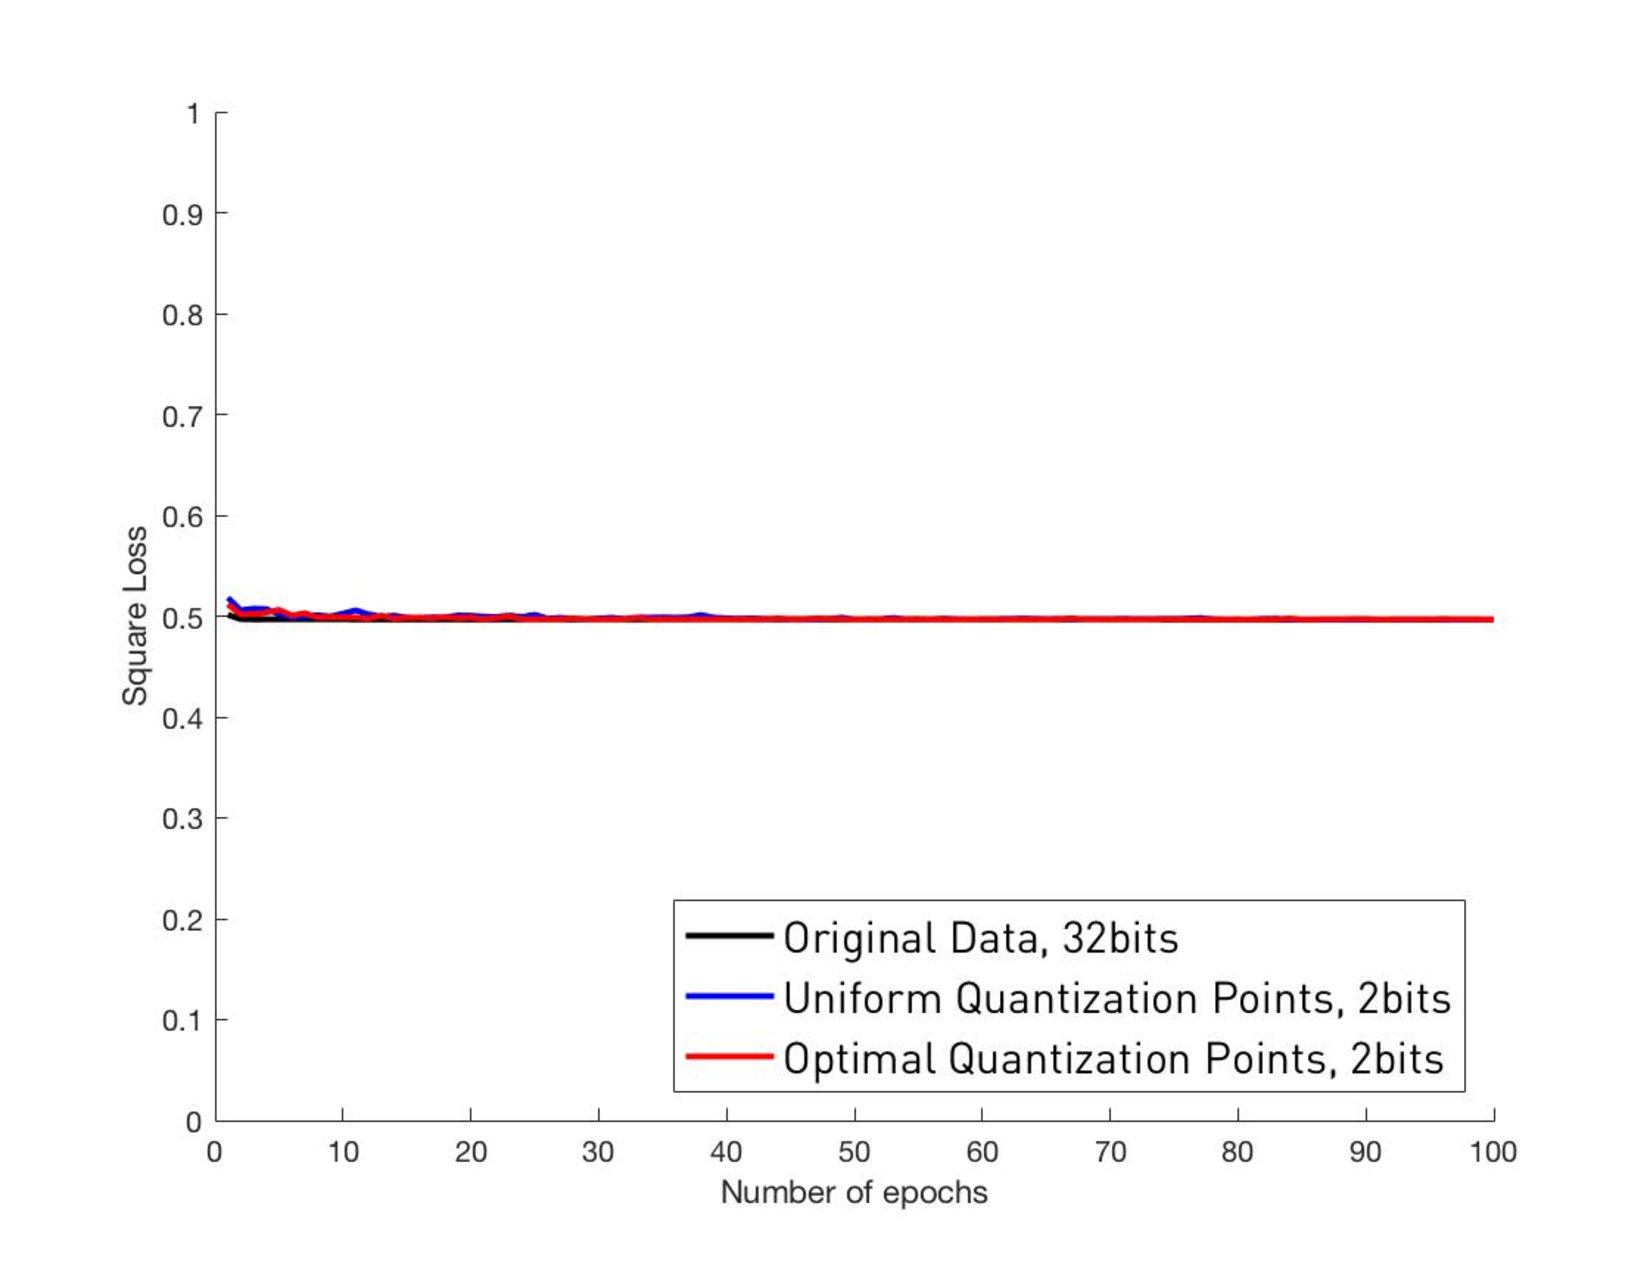
\includegraphics[width=\columnwidth]{additional/syn10-data}
    \caption{Synthetic 10 dataset}
    \end{subfigure}
    \begin{subfigure}[h]{.4\columnwidth}
    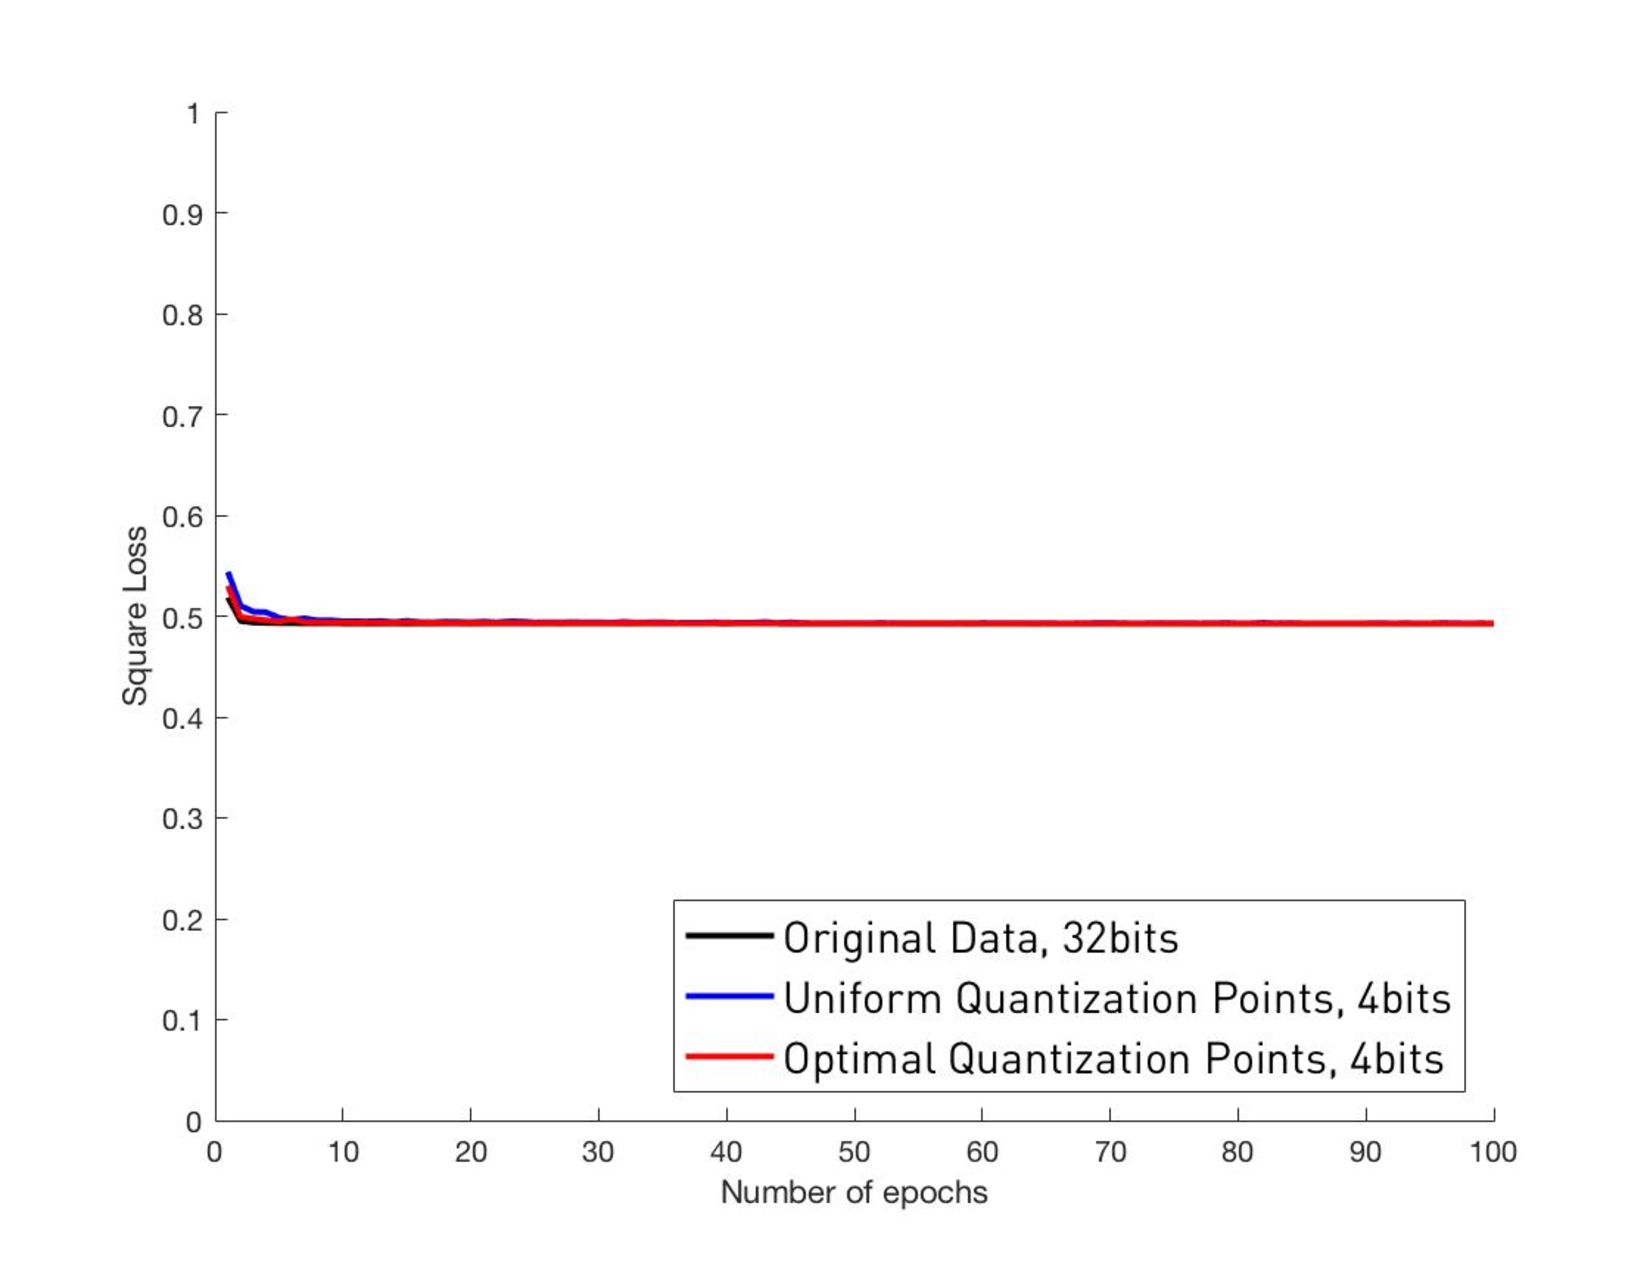
\includegraphics[width=\columnwidth]{additional/syn100-data}
    \caption{Synthetic 100 dataset}
    \end{subfigure}

    \begin{subfigure}[h]{.4\columnwidth}
    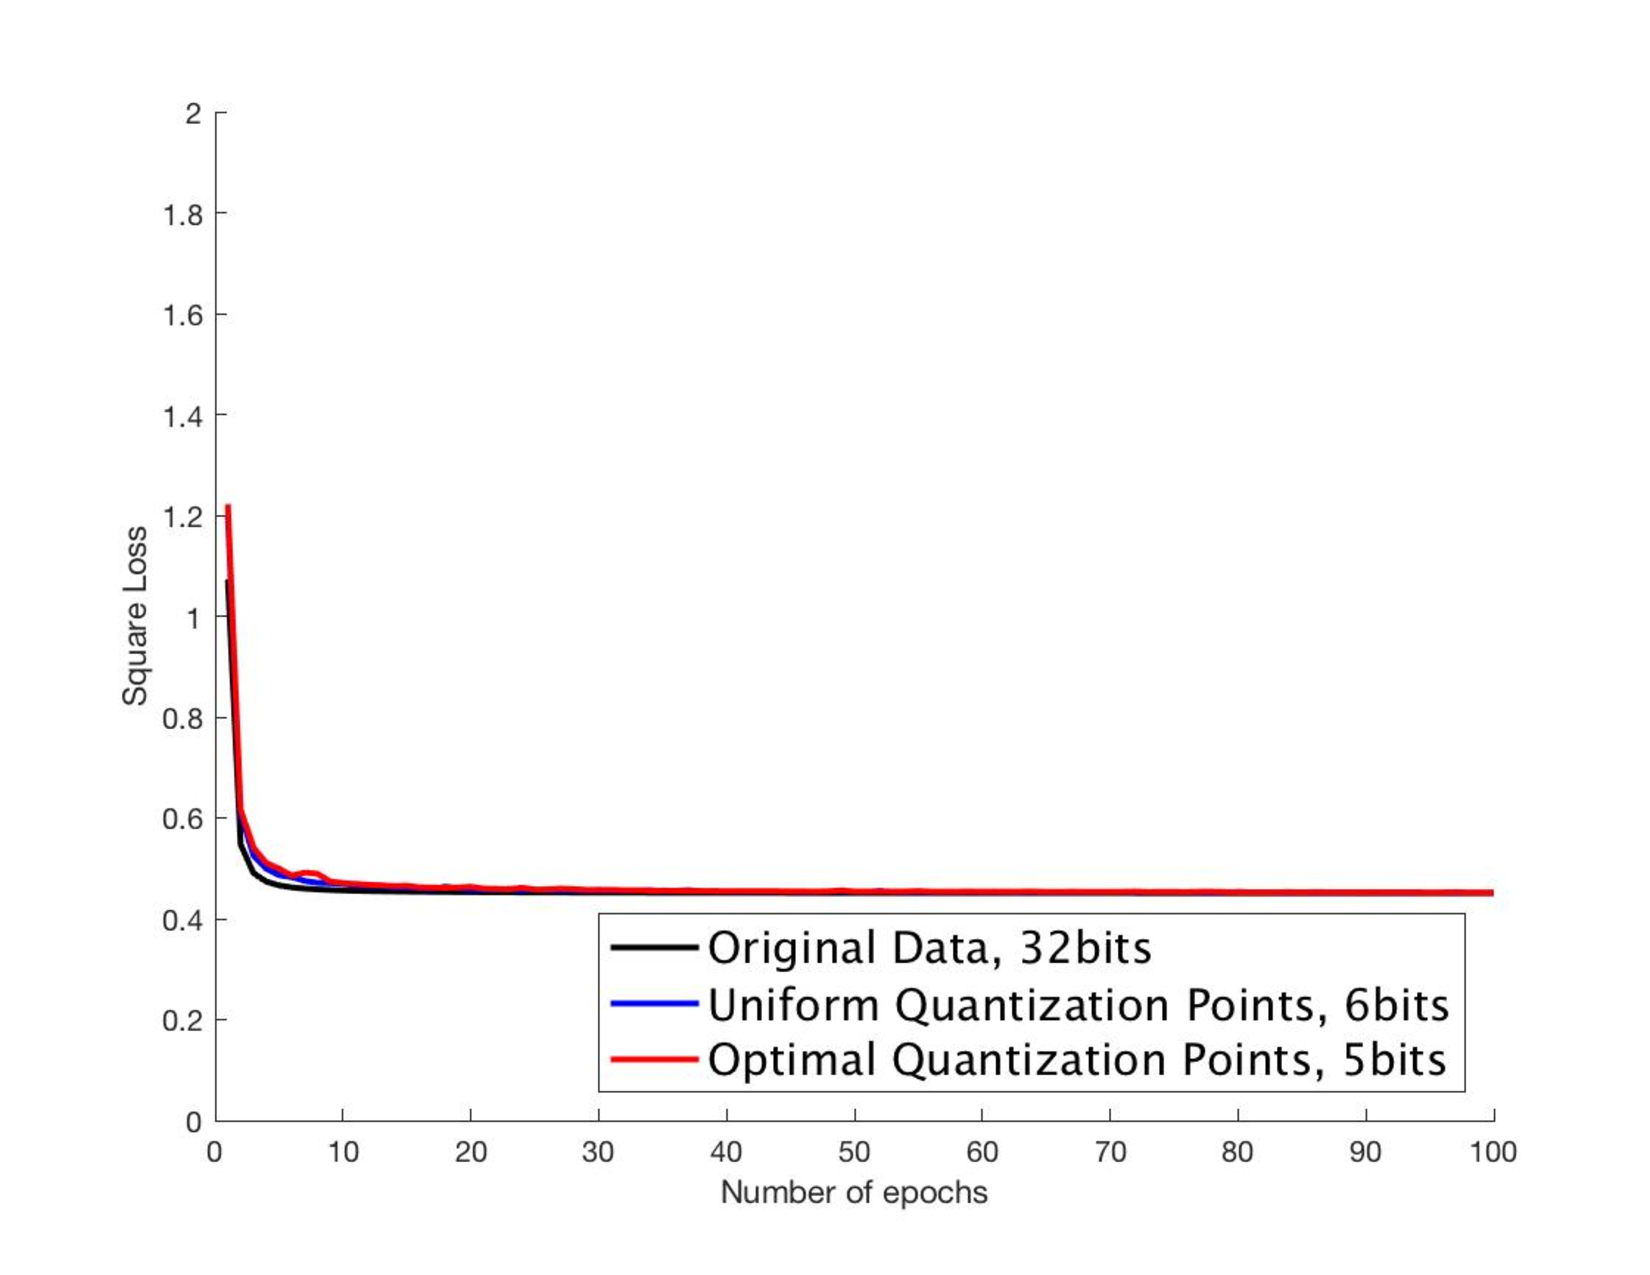
\includegraphics[width=\columnwidth]{additional/syn1000-data}
     \caption{Synthetic 1000 dataset}
    \end{subfigure}
    \begin{subfigure}[h]{.4\columnwidth}
    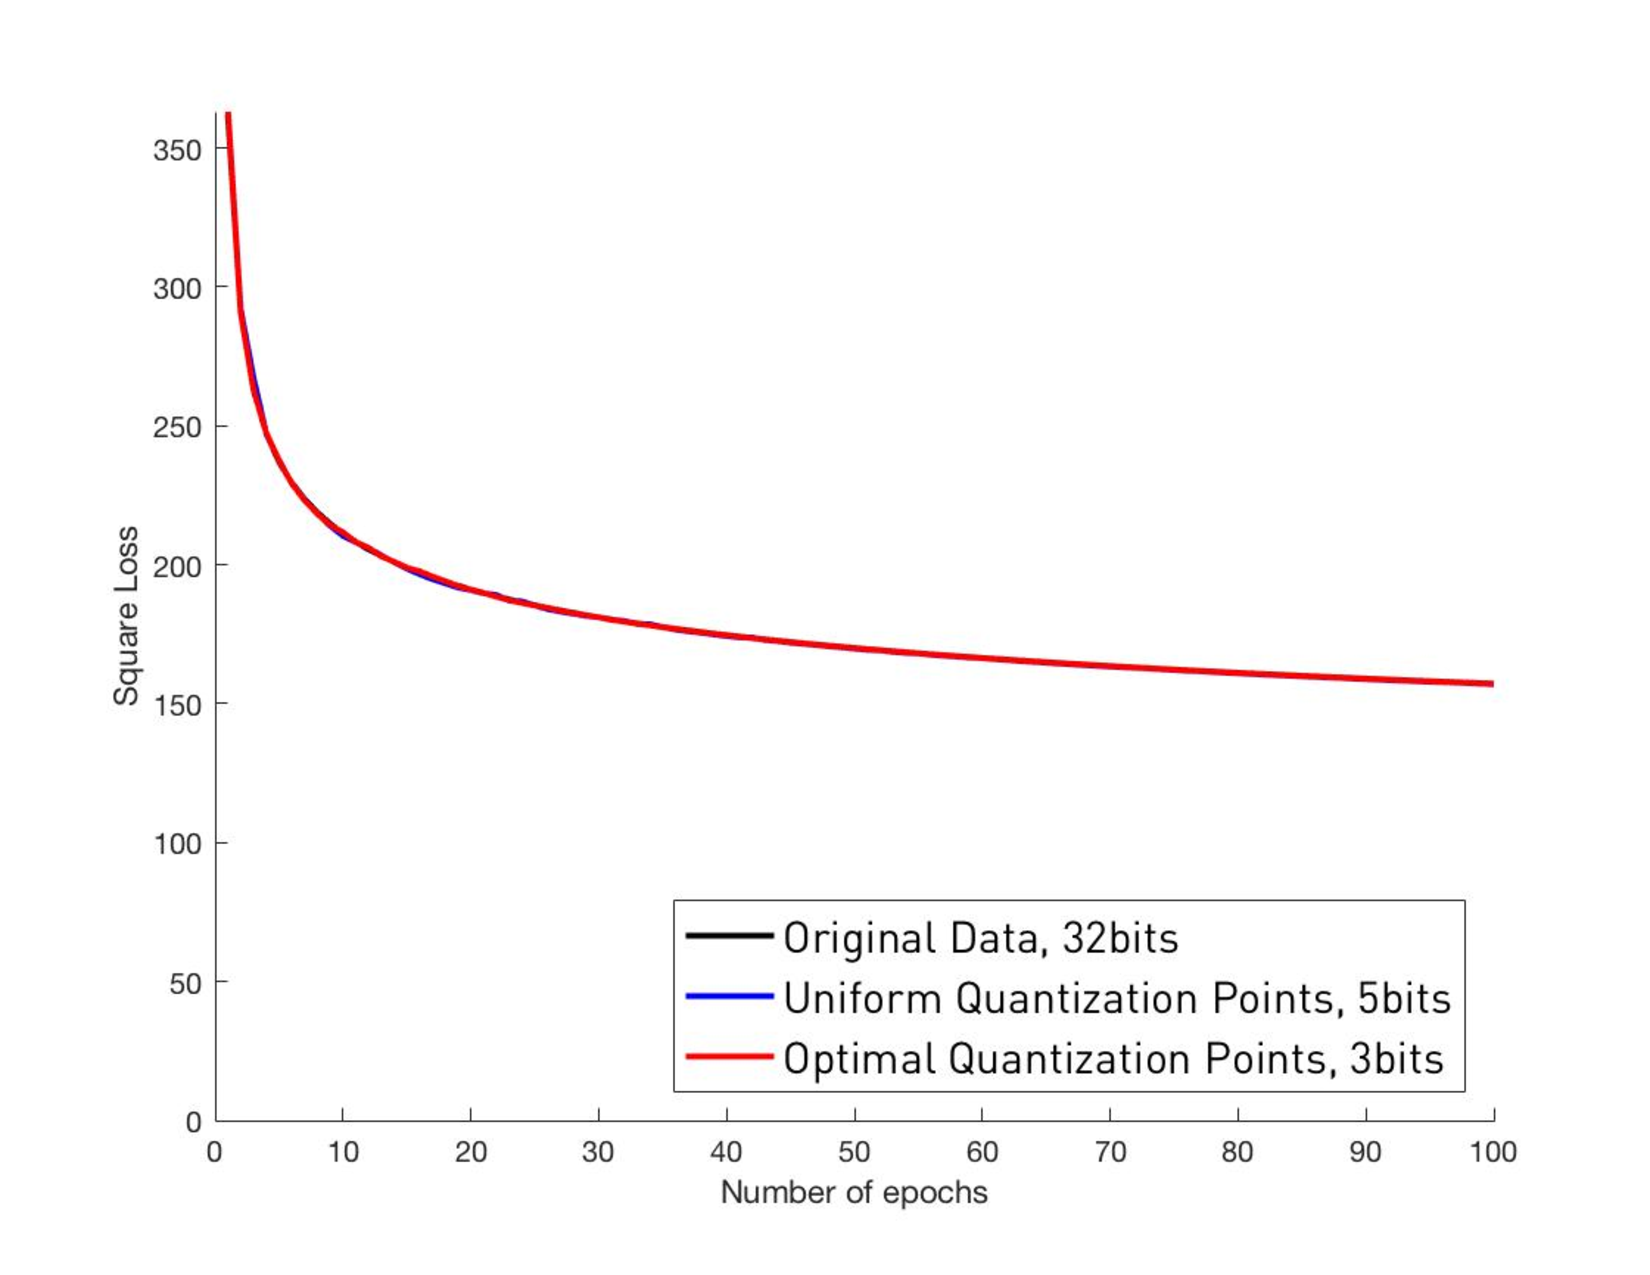
\includegraphics[width=\columnwidth]{additional/year-data}
    \caption{YearPredictionMSD dataset}
    \end{subfigure}

    \begin{subfigure}[h]{.4\columnwidth}
    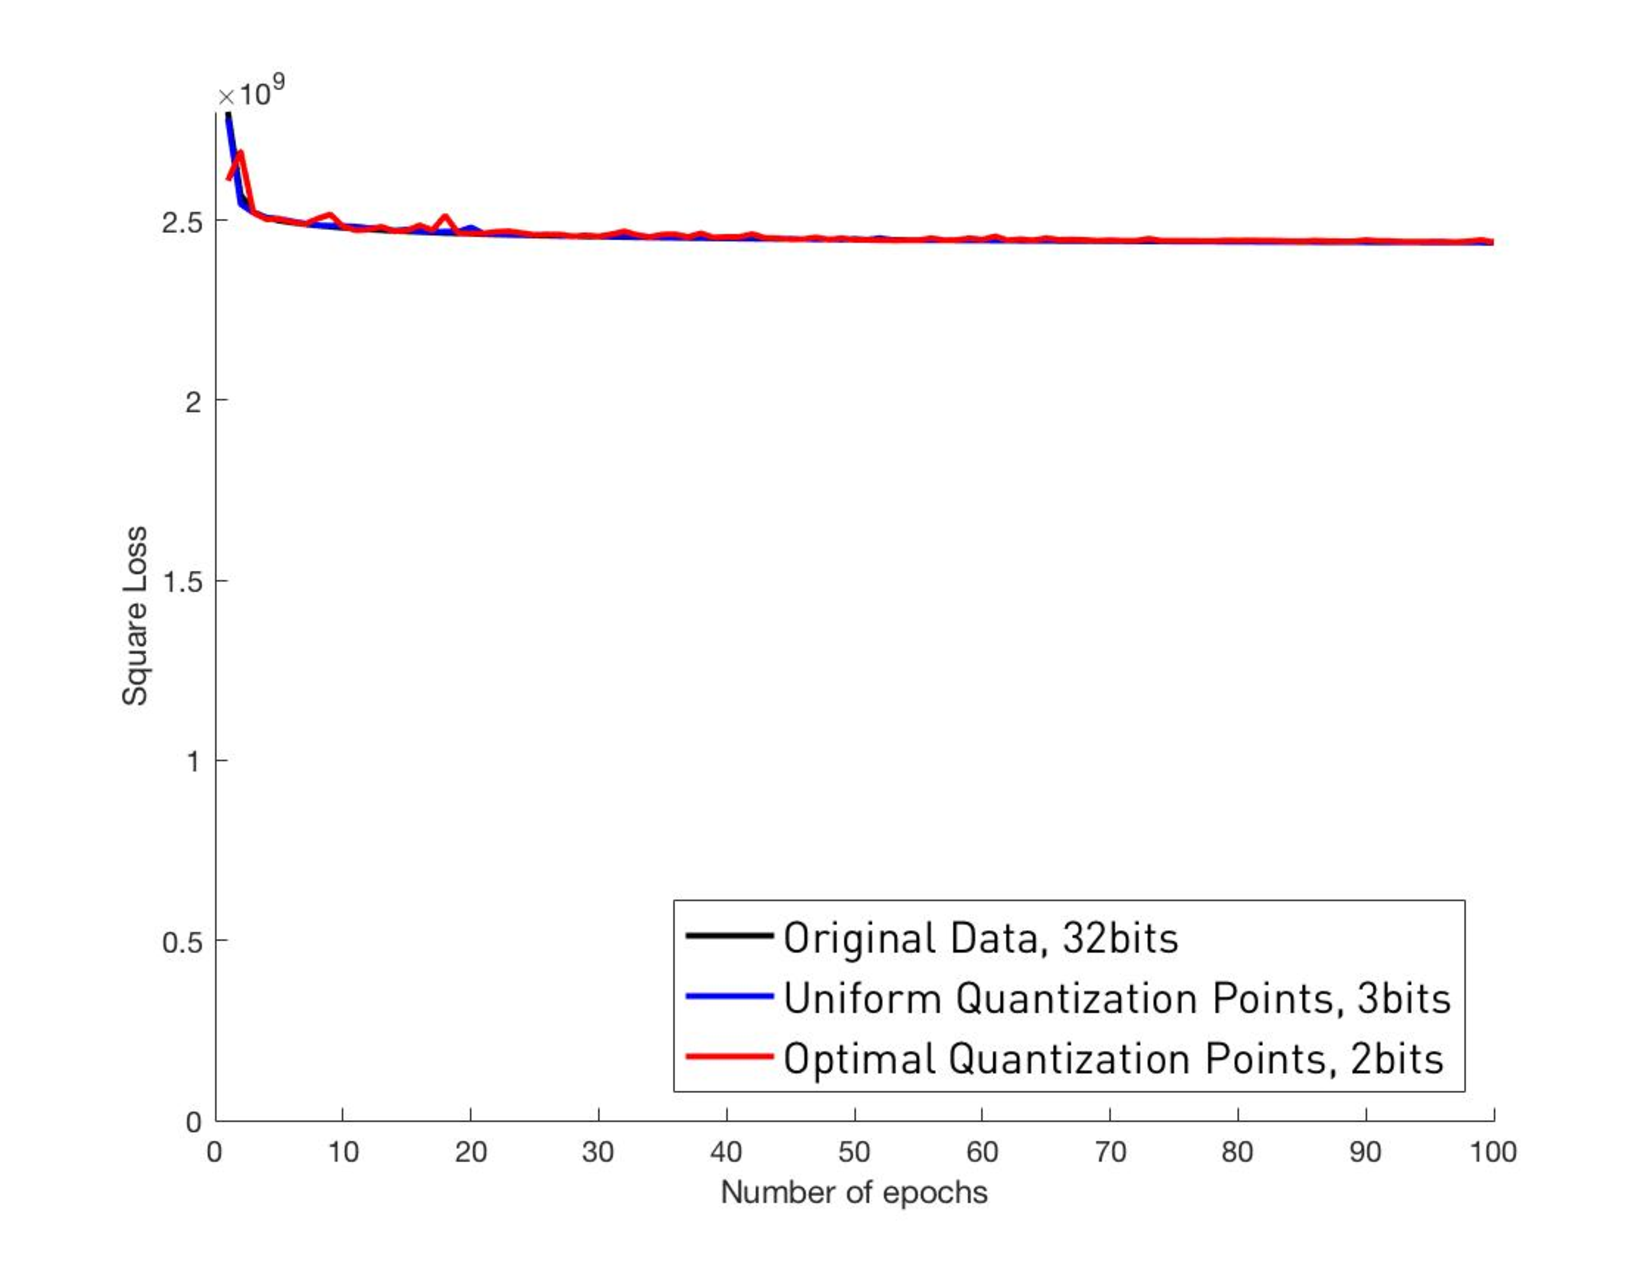
\includegraphics[width=\columnwidth]{additional/cadata-data}
    \caption{cadata dataset}
    \end{subfigure}
    \begin{subfigure}[h]{.4\columnwidth}
    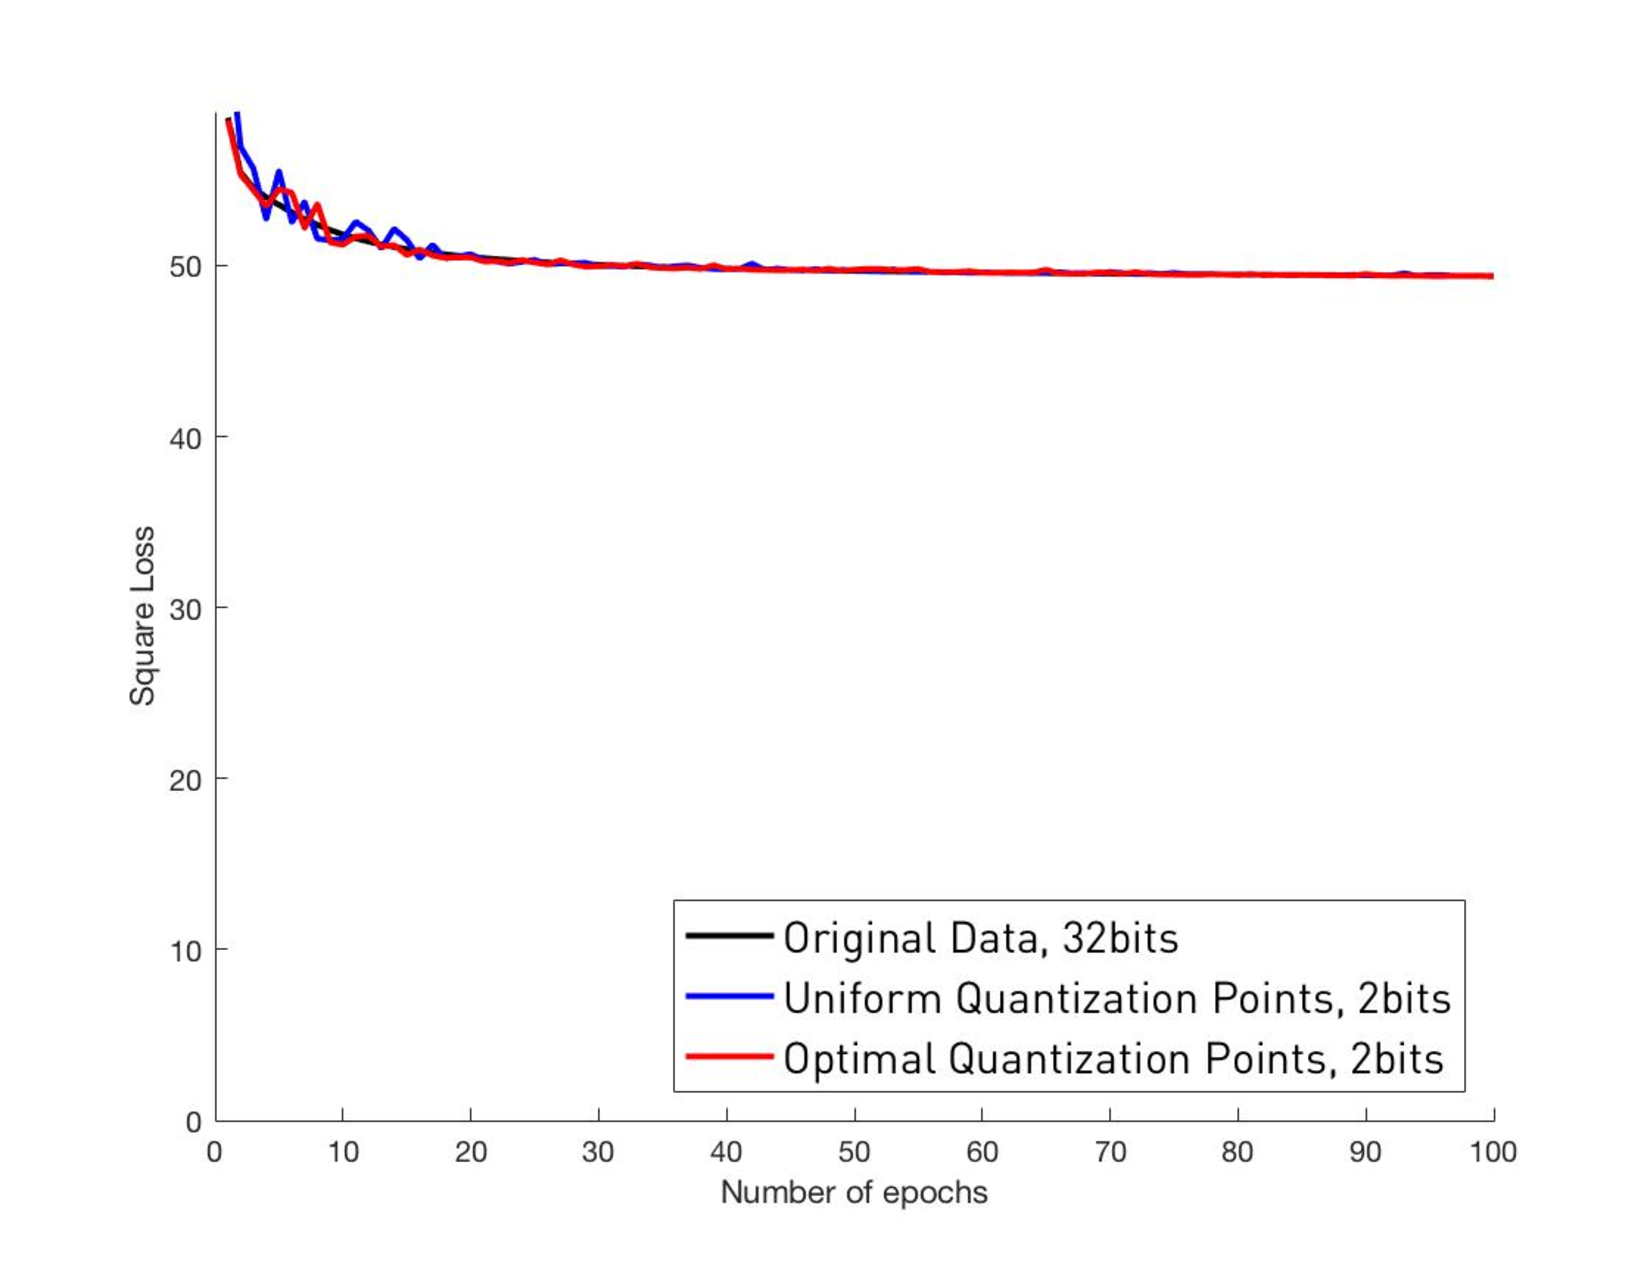
\includegraphics[width=\columnwidth]{additional/cpusmall-data}
     \caption{cpusmall dataset}
    \end{subfigure}
    
\caption{Linear models with low precision data}
\label{fig:lindata}
\end{figure}


\begin{figure}[t]
\centering
    \begin{subfigure}[h]{.4\columnwidth}
    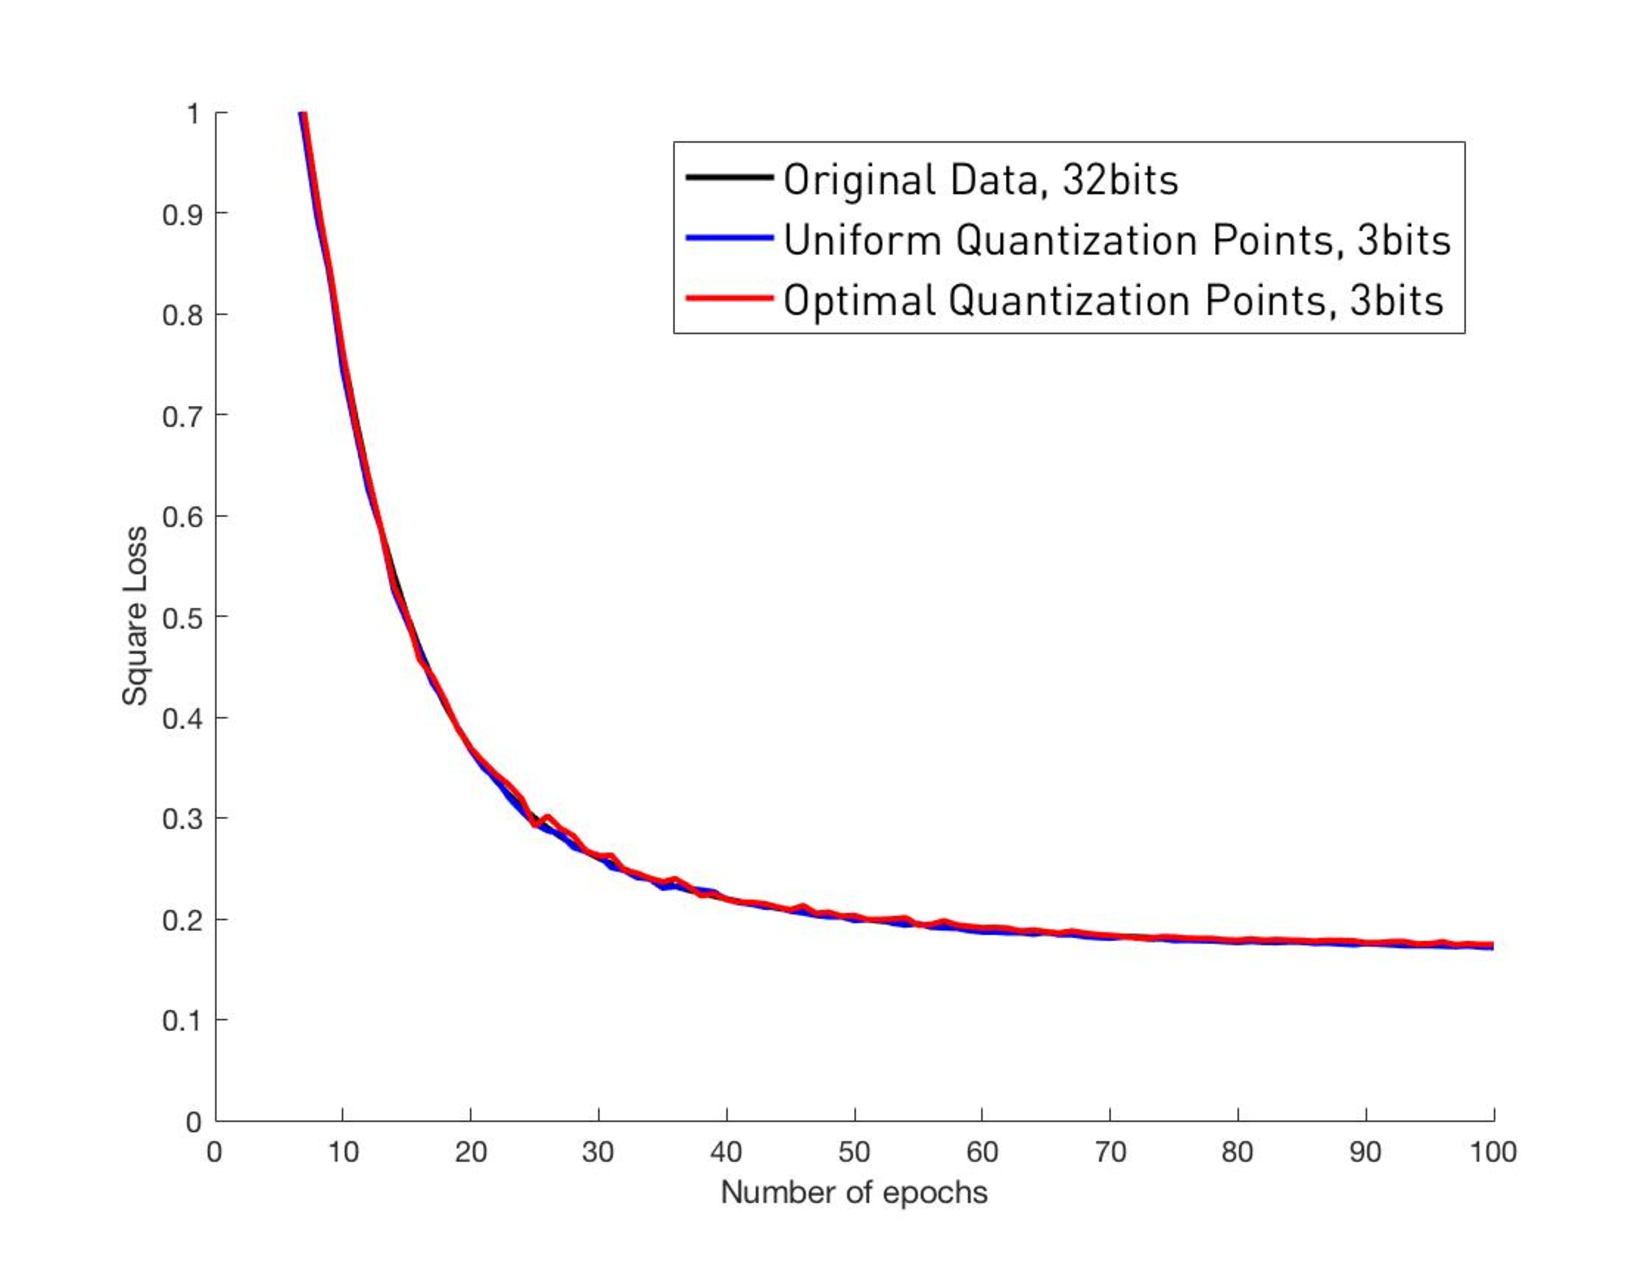
\includegraphics[width=\columnwidth]{additional/cod-rna-data}
    \caption{cod-rna dataset}
    \end{subfigure}
    \begin{subfigure}[h]{.4\columnwidth}
    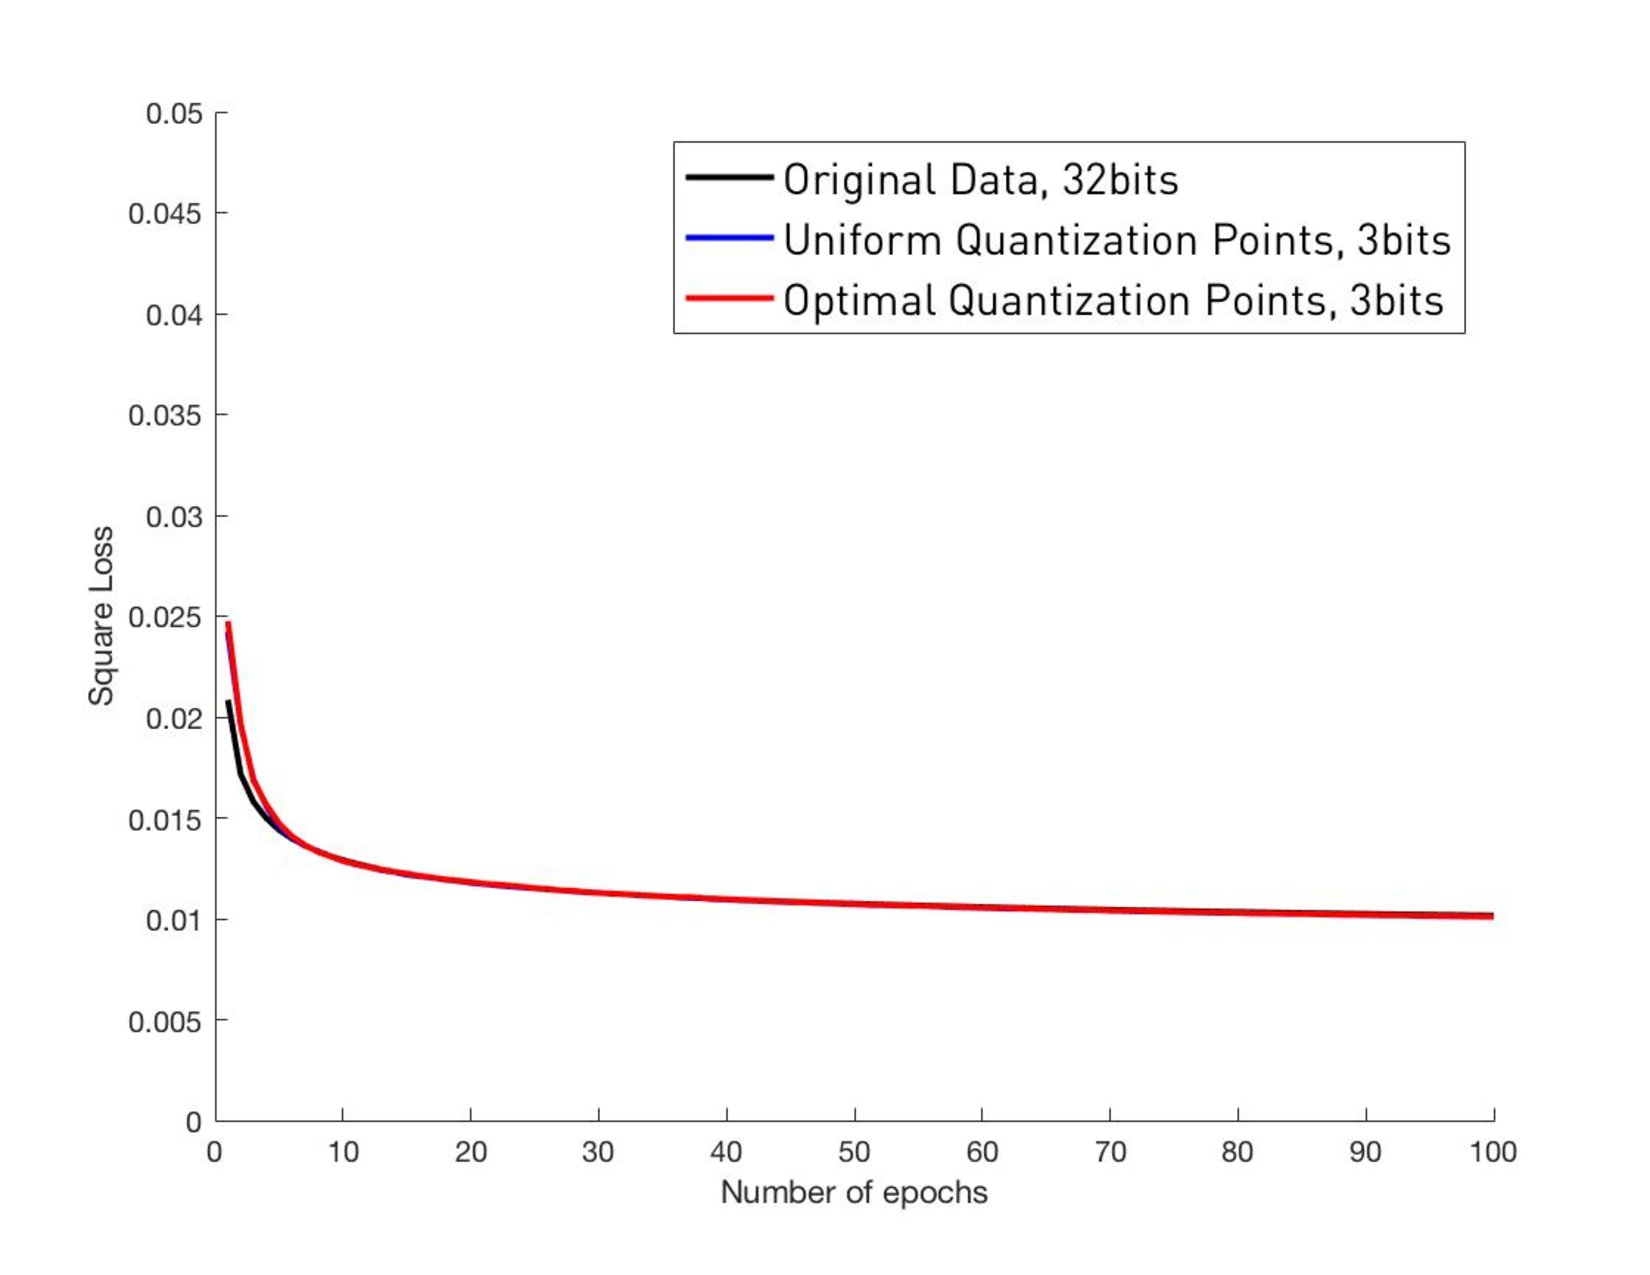
\includegraphics[width=\columnwidth]{additional/gisette-data}
    \caption{gisette dataset}
    \end{subfigure}    
\caption{Least Squares SVM with low precision data}
\label{fig:lssvmdata}
\end{figure}

\paragraph{End-to-End Quantization}
We validate that (1) if we quantize data with double sampling, SGD with low precision converges---in comparable empirical 
convergence rates---to the same solution as SGD with full precision.

Figure~\ref{fig:linendtoend}-\ref{fig:lssvmendtoend} illustrates that the result of training linear models:
(a) linear regression and (b) least squares SVMs,
with end-to-end low precision and 
full precision. For low precision, we pick the 
smallest number of bits that results in a smooth convergence
curve. We compare the final training loss in both settings and the convergence rate.


We see that, for both linear regression 
and least squares SVM,
using 4-6 bits is always enough
to converge to the same solution
with comparable convergence rate. 
And when we compare the end-to-end quantization
with quantized data, we can see that we
need more bits, which is because the extra variance introduced
by quantized model and gradient. 
\begin{figure}[t]
\centering
    \begin{subfigure}[h]{.4\columnwidth}
    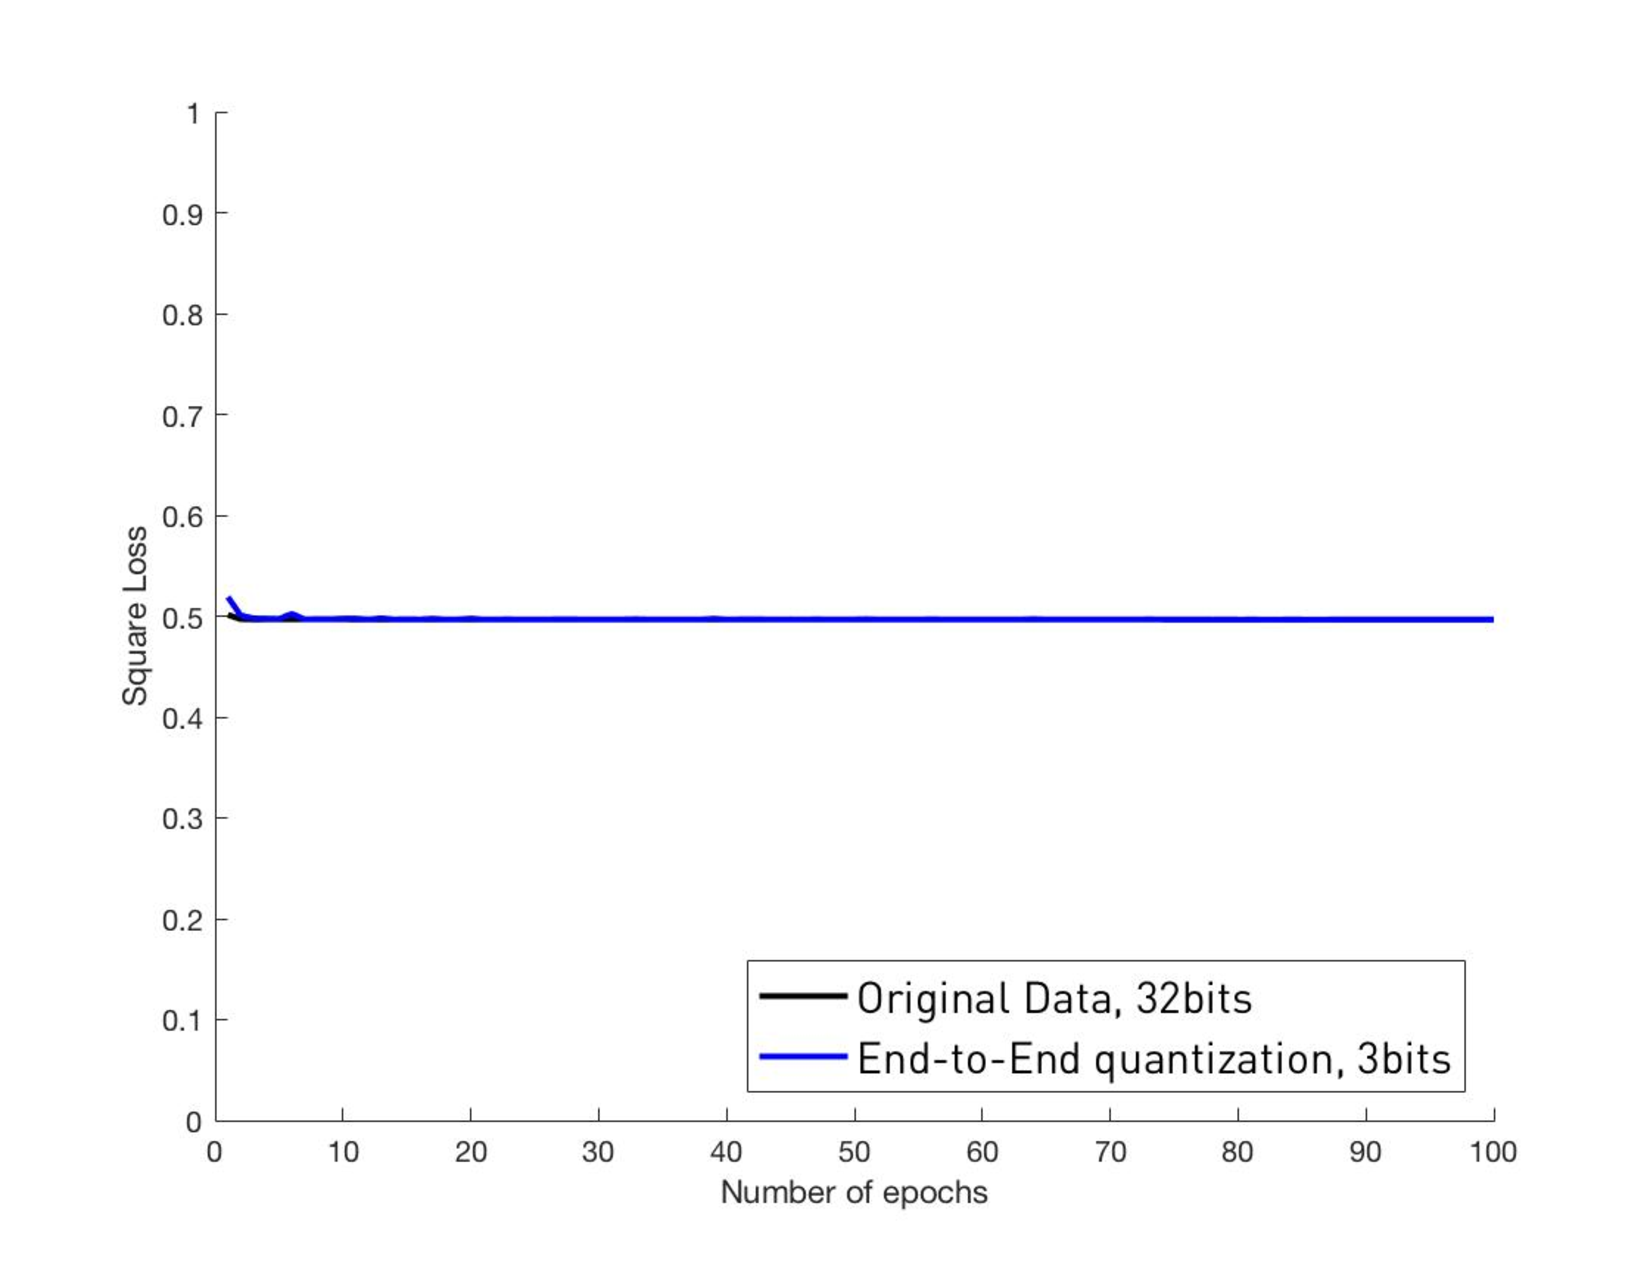
\includegraphics[width=\columnwidth]{additional/syn10-endtoend}
    \caption{Synthetic 10 dataset}
    \end{subfigure}
    \begin{subfigure}[h]{.4\columnwidth}
    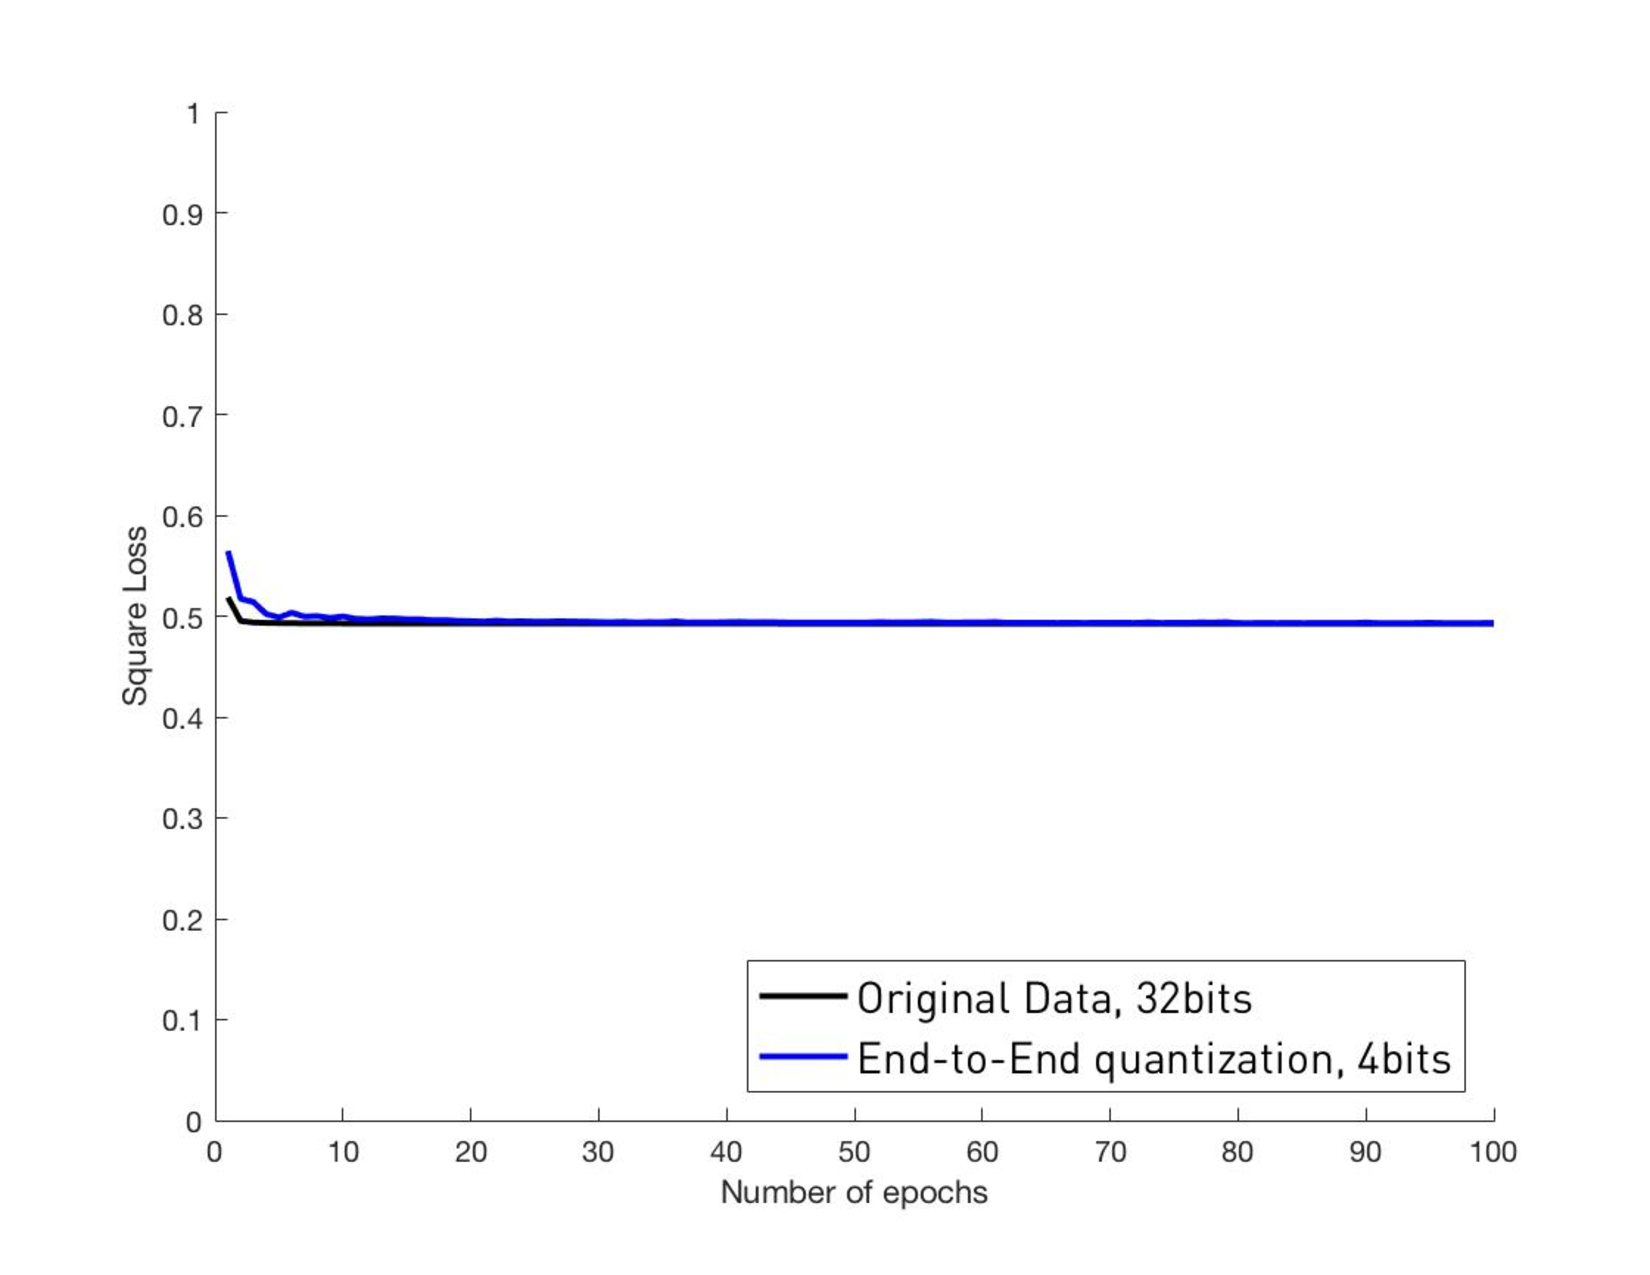
\includegraphics[width=\columnwidth]{additional/syn100-endtoend}
    \caption{Synthetic 100 dataset}
    \end{subfigure}

    \begin{subfigure}[h]{.4\columnwidth}
    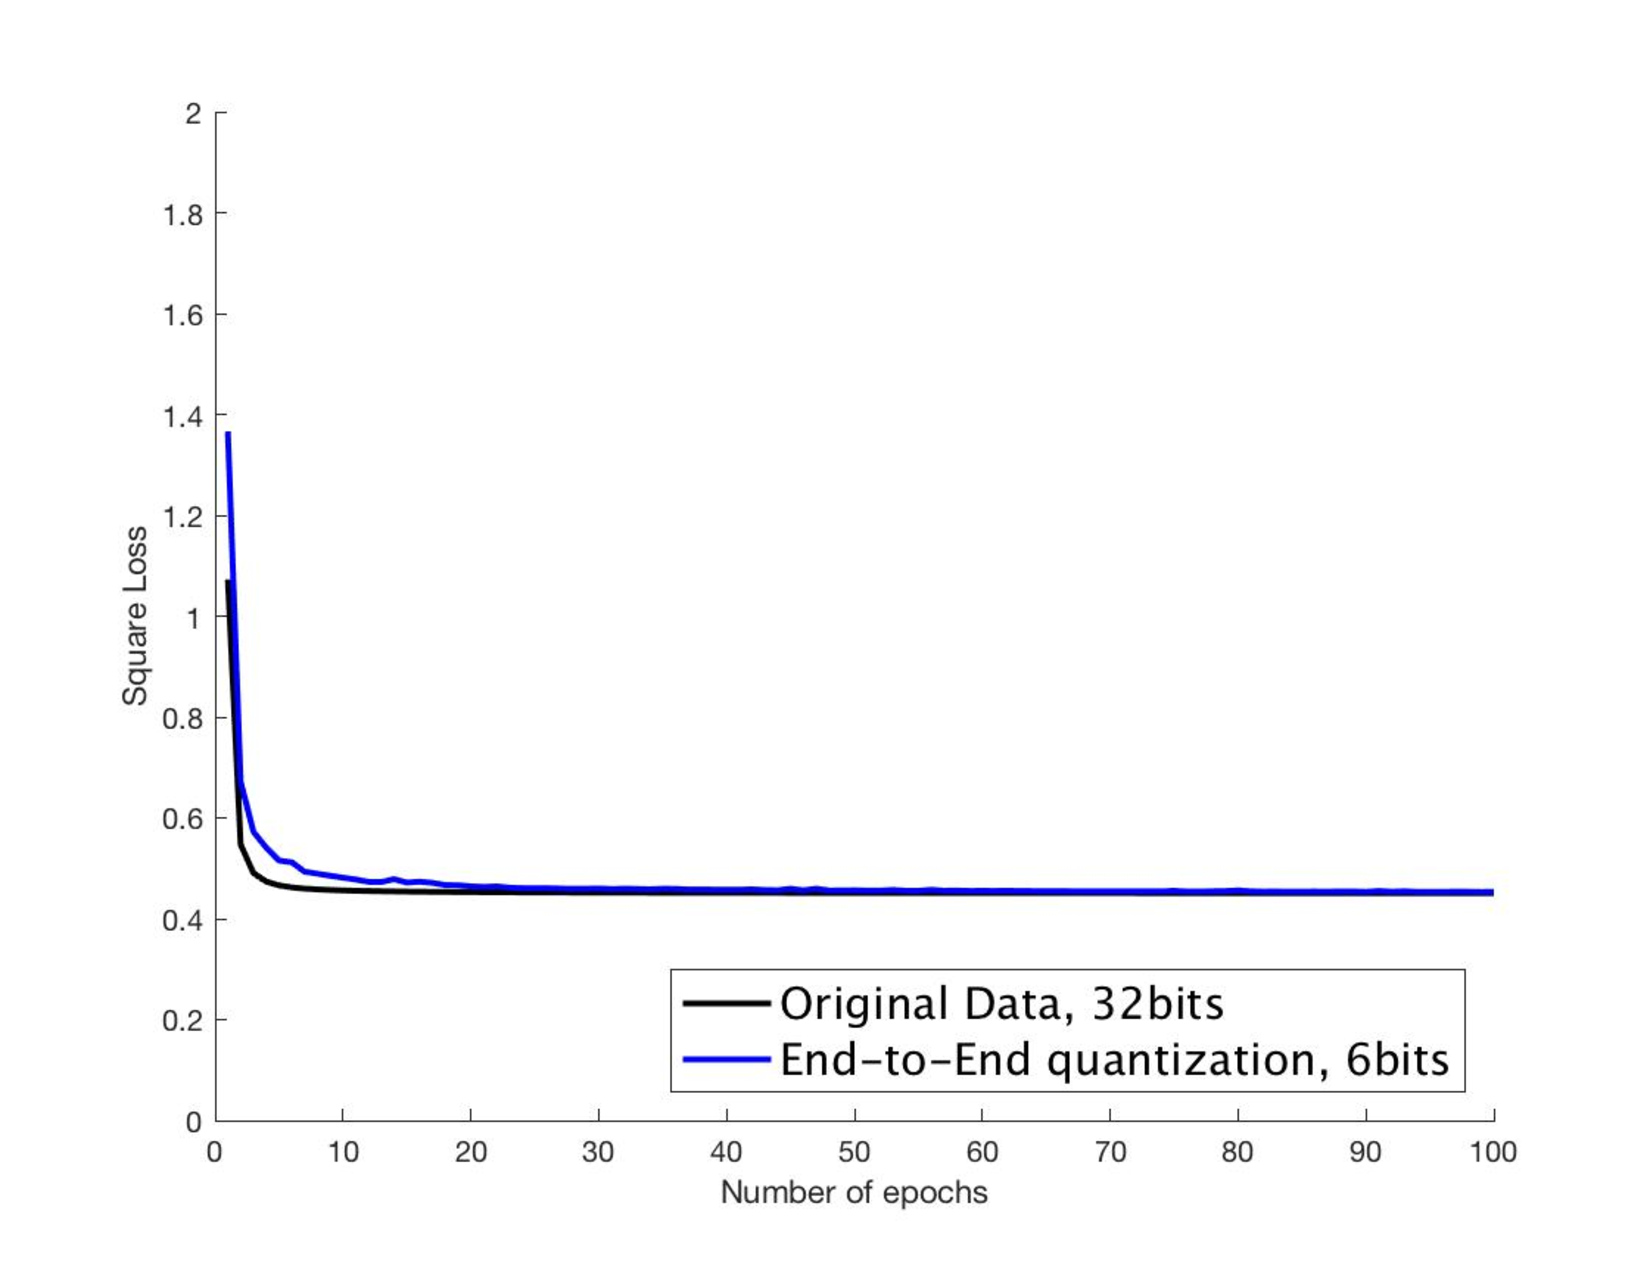
\includegraphics[width=\columnwidth]{additional/syn1000-endtoend}
     \caption{Synthetic 1000 dataset}
    \end{subfigure}
    \begin{subfigure}[h]{.4\columnwidth}
    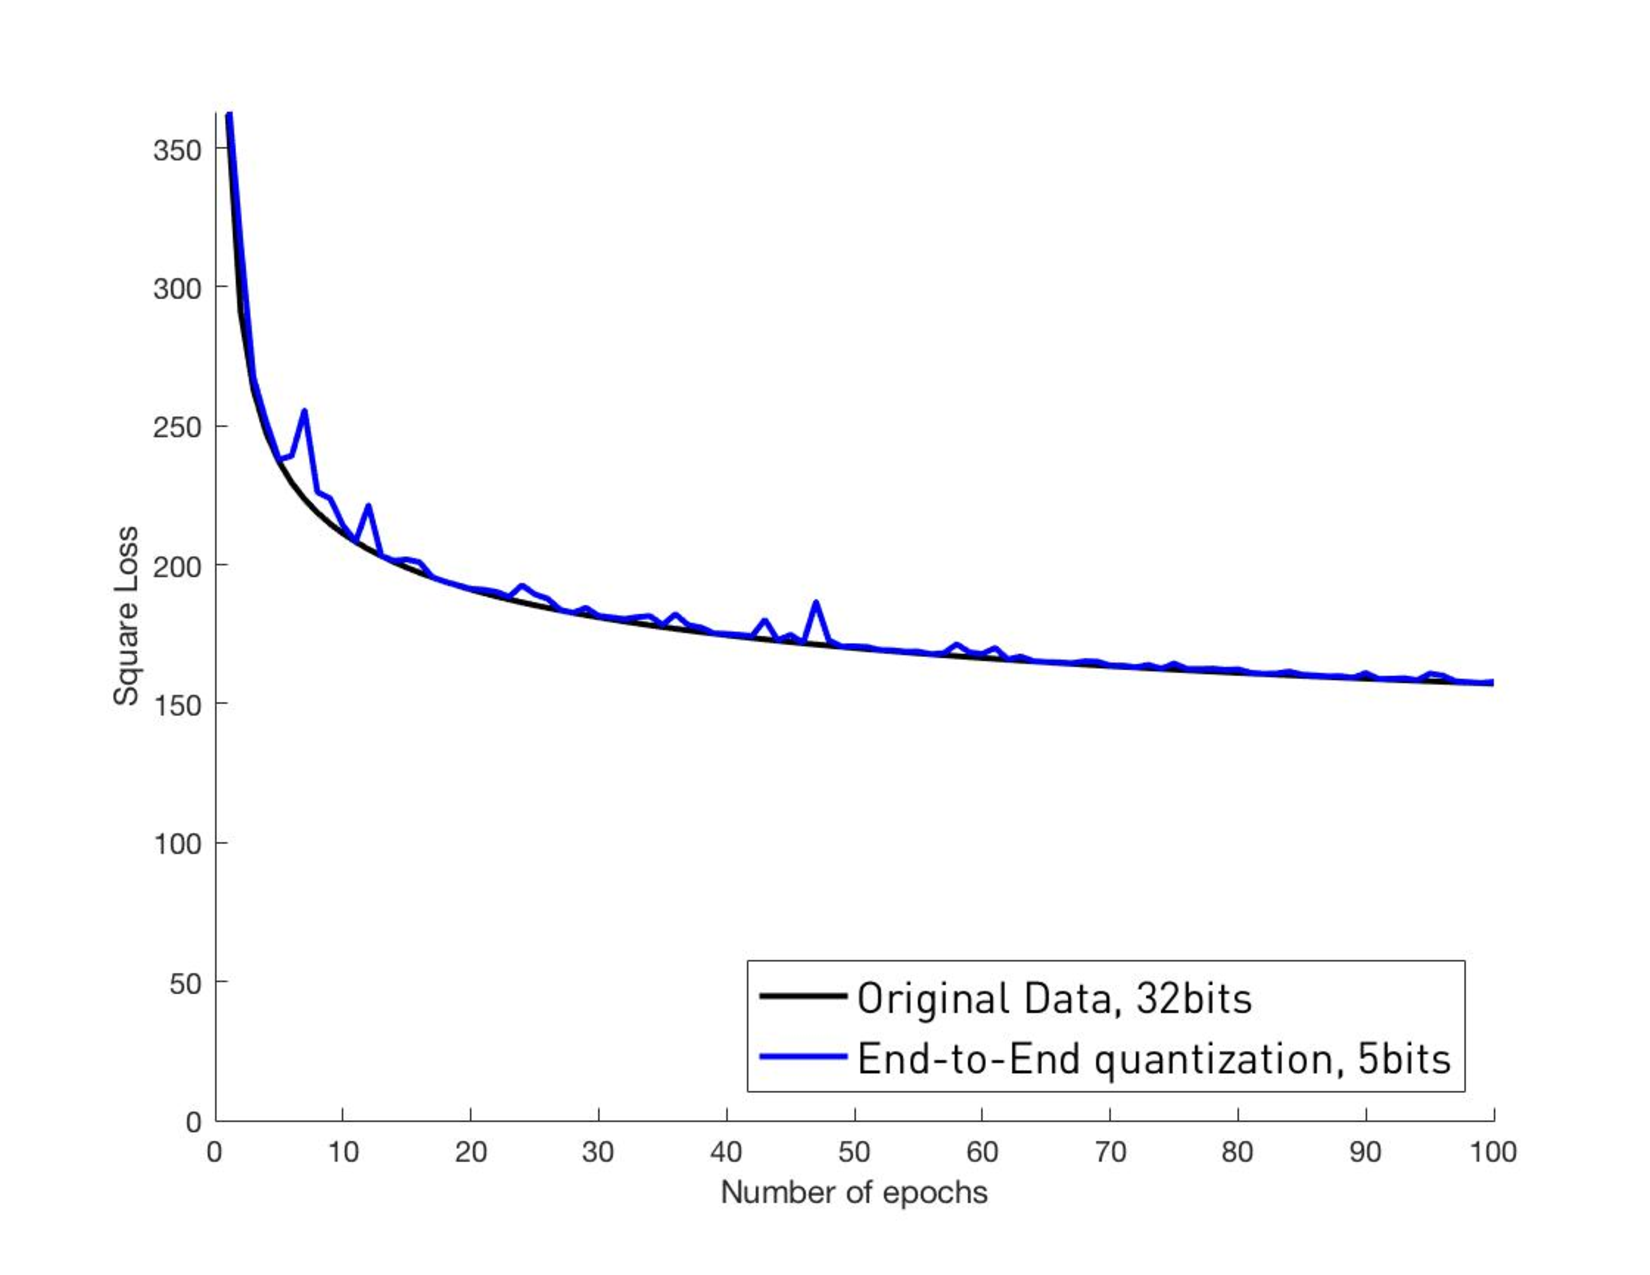
\includegraphics[width=\columnwidth]{additional/year-endtoend}
    \caption{YearPredictionMSD dataset}
    \end{subfigure}
    
    \begin{subfigure}[h]{.4\columnwidth}
    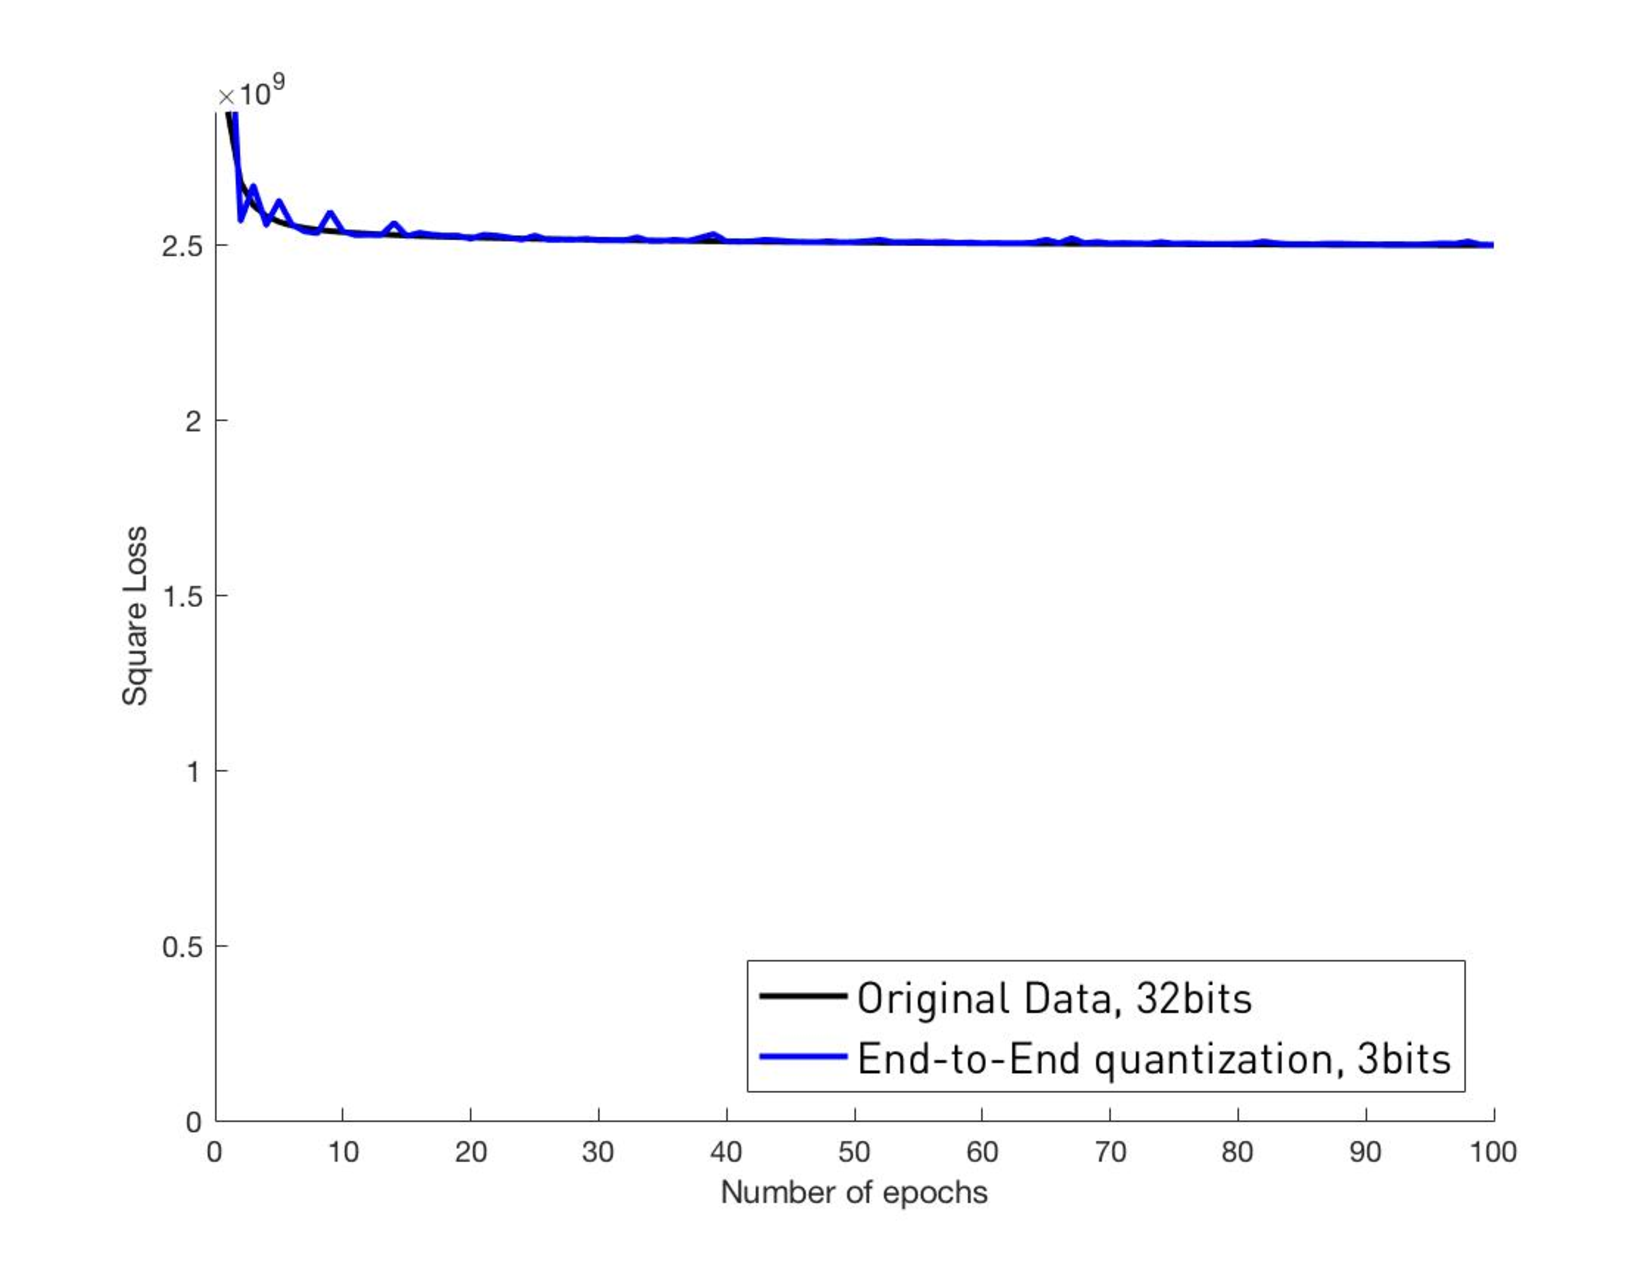
\includegraphics[width=\columnwidth]{additional/cadata-endtoend}
    \caption{cadata dataset}
    \end{subfigure}
    \begin{subfigure}[h]{.4\columnwidth}
    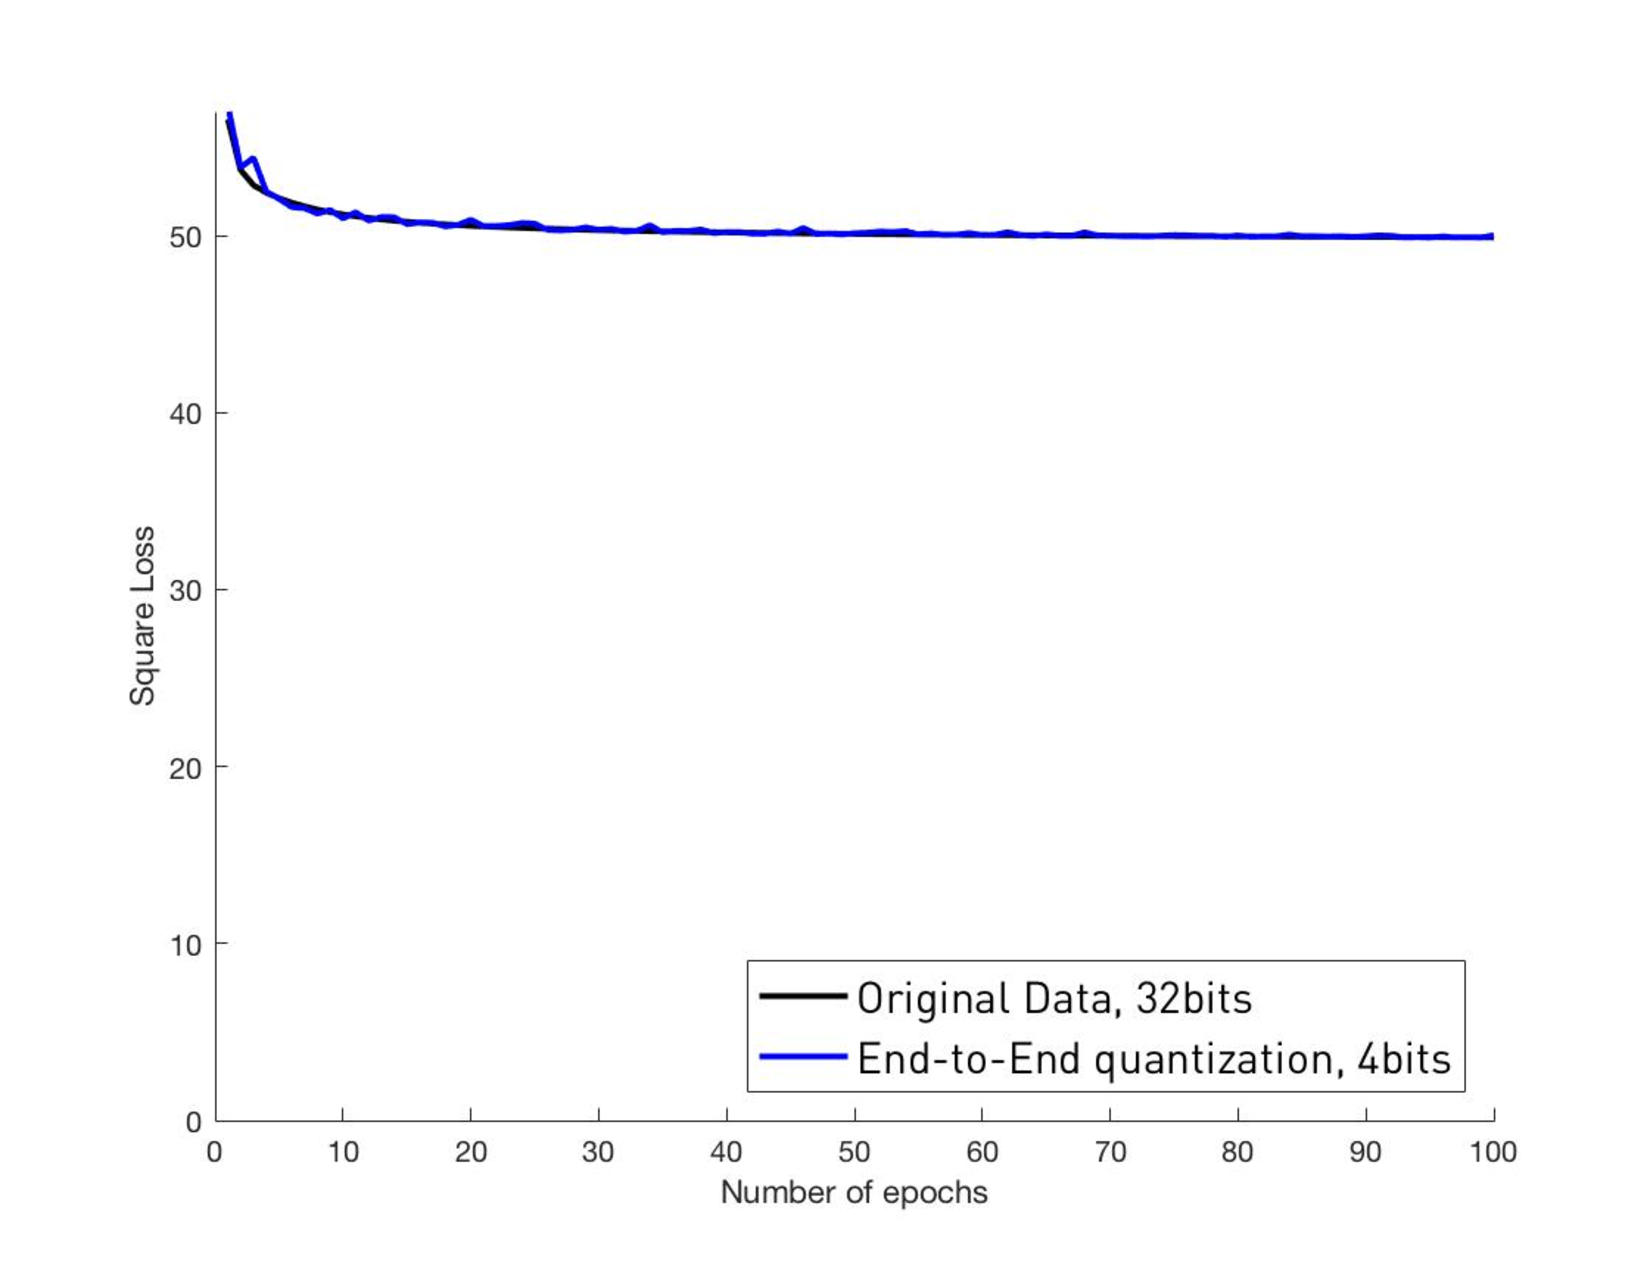
\includegraphics[width=\columnwidth]{additional/cpusmall-endtoend}
     \caption{cpusmall dataset}
    \end{subfigure}
    
\caption{Linear models with end-to-end low precision}
\label{fig:linendtoend}
\end{figure}


\begin{figure}[t]
\centering
    \begin{subfigure}[h]{.4\columnwidth}
    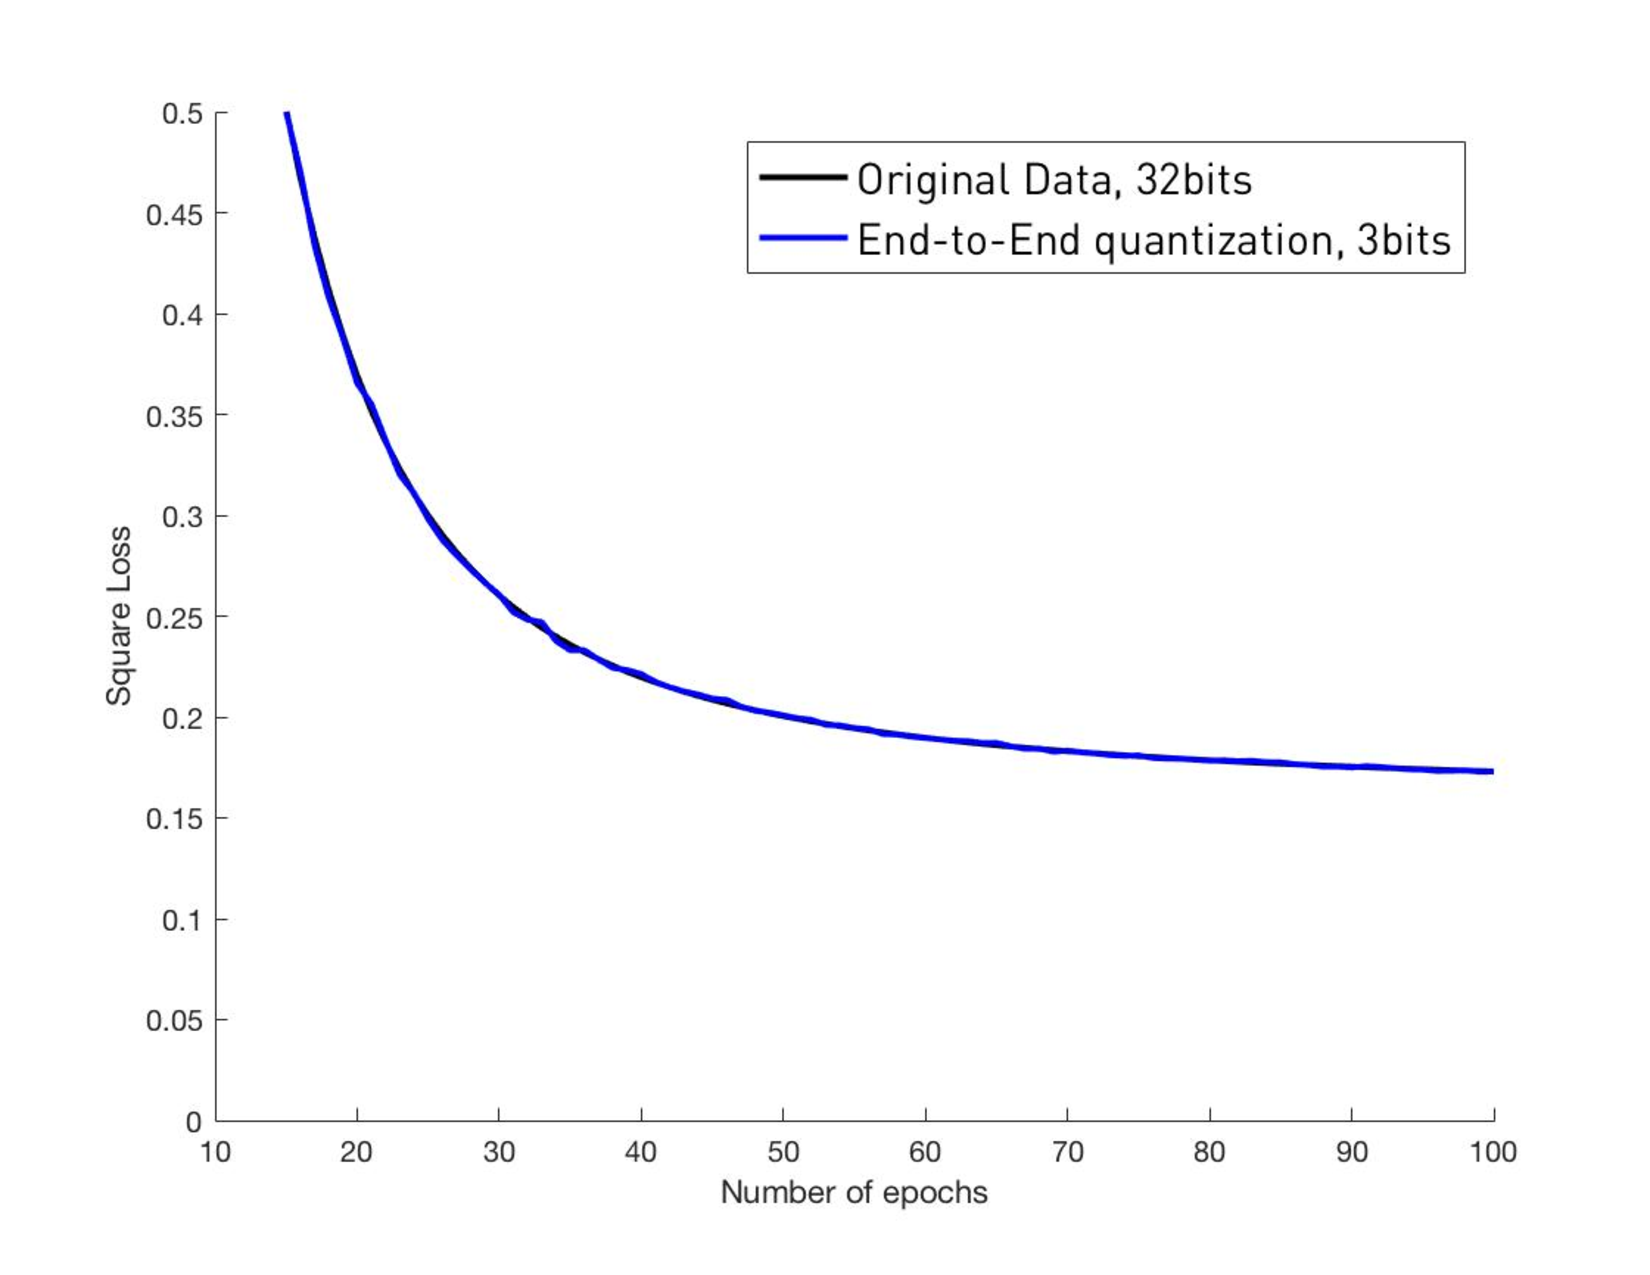
\includegraphics[width=\columnwidth]{additional/cod-rna-endtoend}
    \caption{cod-rna dataset}
    \end{subfigure}
    \begin{subfigure}[h]{.4\columnwidth}
    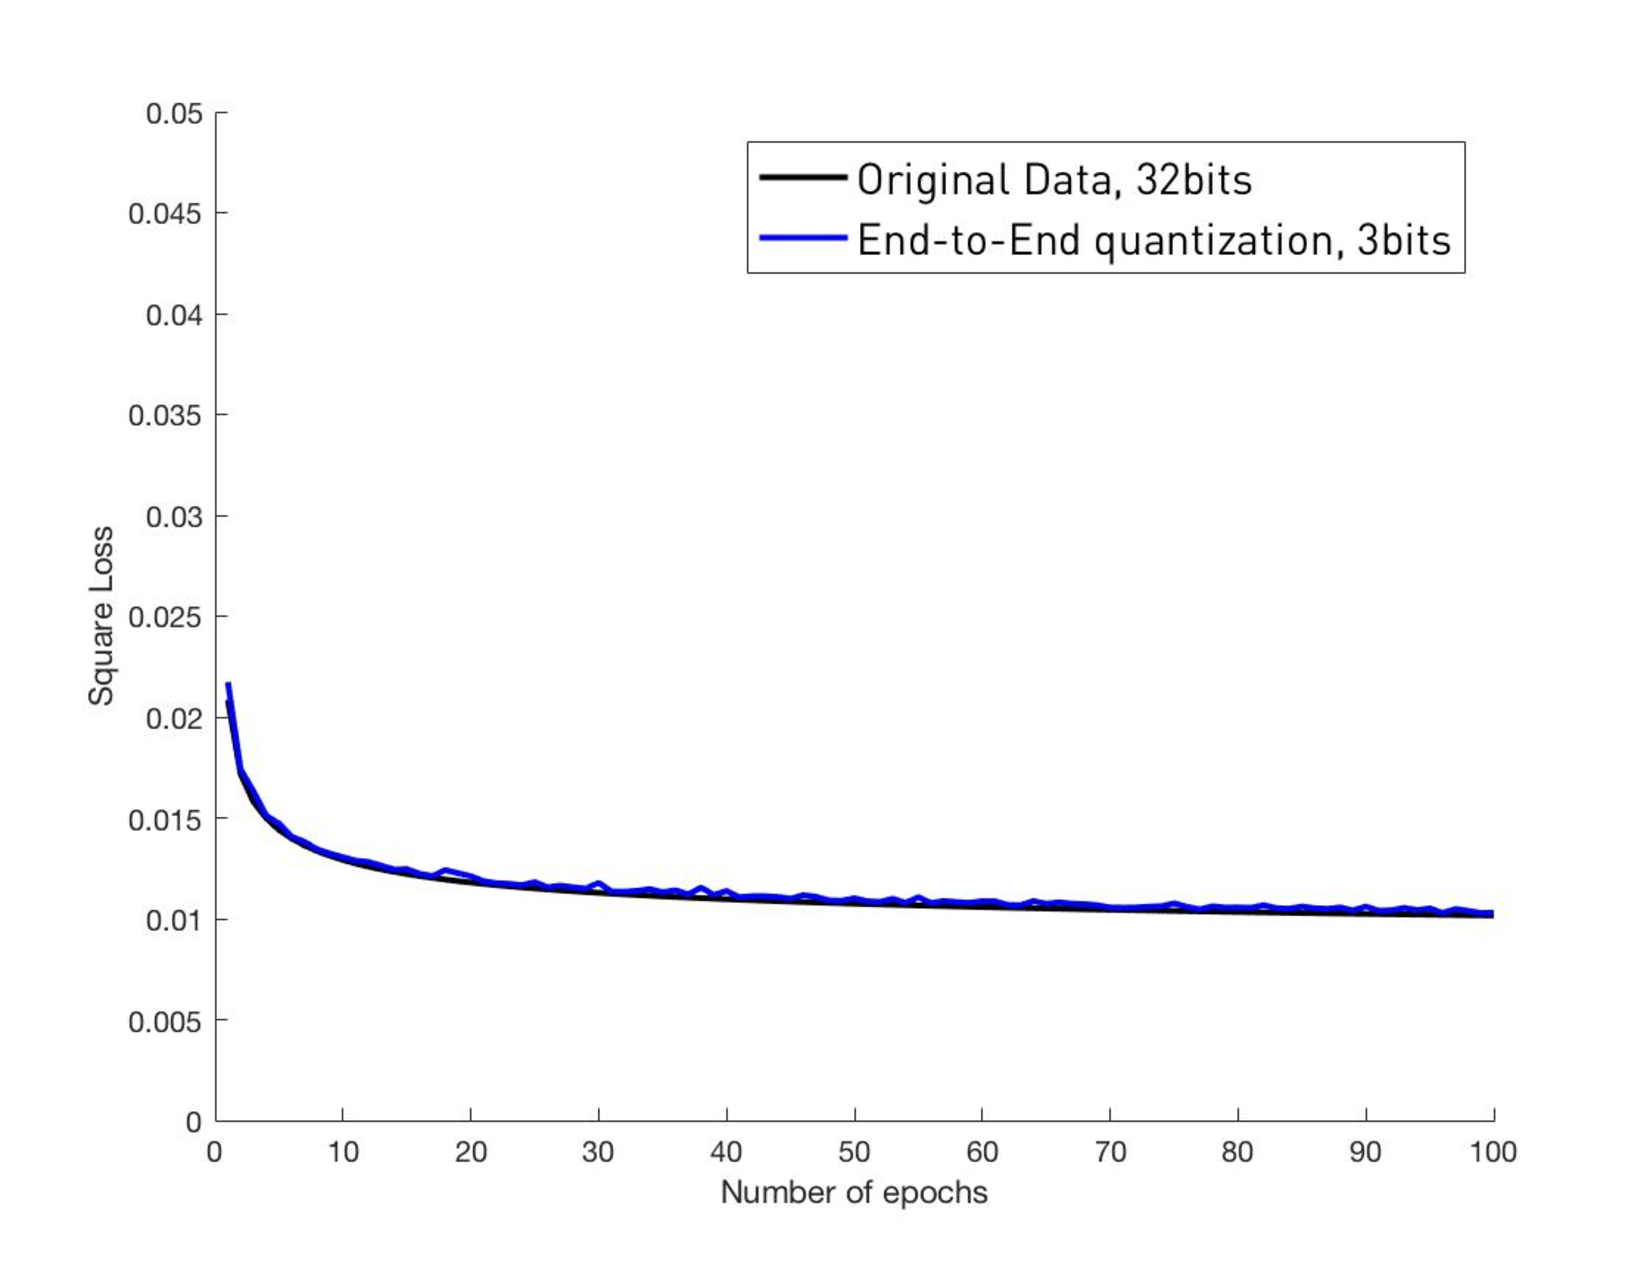
\includegraphics[width=\columnwidth]{additional/gisette-endtoend}
    \caption{gisette dataset}
    \end{subfigure}
    
\caption{Least Squares SVM with end-to-end low precision}
\label{fig:lssvmendtoend}
\end{figure}

\paragraph{Impact of the number of features}
We can see from figure~\ref{fig:lindata} (a)-(c) shows that with more features, the variance introduced by quantization increases and we need more bits to converge.

\subsection{Non-Linear Models}

We validate that for SVM, we can use our refetching heuristic and we can 
8-bit while only refetching $<10\%$ of the data.

\paragraph{Refetching Heuristic for SVM}

Figure~\ref{fig:refetch} illustrates
the result of training SVM
with refetching heuristic. 
We see that, 
with our refetching heuristic,
SGD converges to similar training loss 
with a comparable empirical convergence 
rate for SVM. If we increase the number of
bits we use, we need to refetch less data and
if we use 8-bit quantization, we only need to fetch
about $6\%$ of data.
We also experience no loss in test accuracy.

\begin{figure}[t]
\centering
    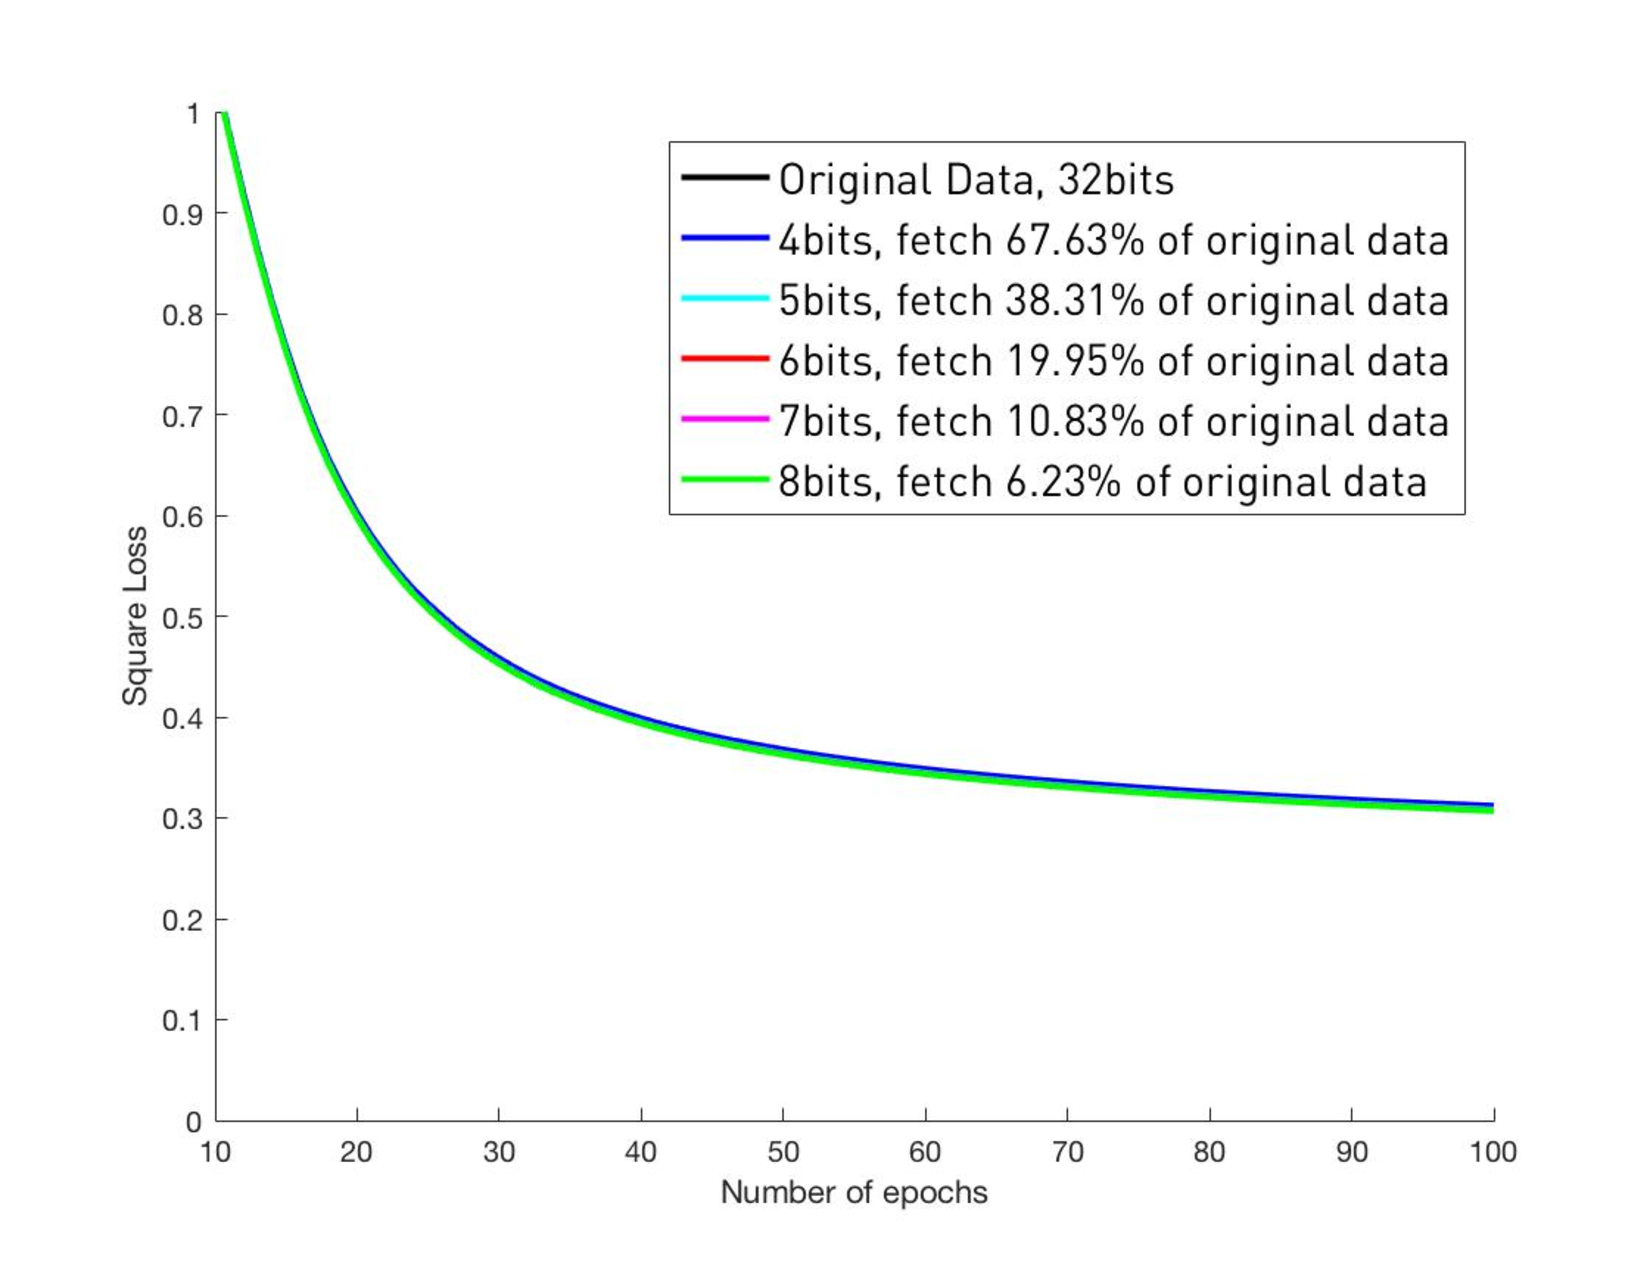
\includegraphics[width=0.5\columnwidth]{additional/fetch}
    
\caption{SVM with low precision data and refetching on cod-rna dataset}
\label{fig:refetch}
\end{figure}

\bibliographystyle{alpha}
\bibliography{low-precision.bib}


\end{document}
